% =====================================================================
% BAB IV — HASIL DAN PEMBAHASAN
% Skripsi: Pengembangan Website Simulasi Wawancara Kerja Berbasis Large
%          Language Model dengan Integrasi Gemini Live API
% Andri Hari Musyaffa — 2802607722
%
% Berkas ini dapat dikompilasi sendiri (tectonic bab4.tex / xelatex bab4.tex)
% maupun disisipkan ke dokumen skripsi utama dengan % =====================================================================
% BAB IV — HASIL DAN PEMBAHASAN
% Skripsi: Pengembangan Website Simulasi Wawancara Kerja Berbasis Large
%          Language Model dengan Integrasi Gemini Live API
% Andri Hari Musyaffa — 2802607722
%
% Berkas ini dapat dikompilasi sendiri (tectonic bab4.tex / xelatex bab4.tex)
% maupun disisipkan ke dokumen skripsi utama dengan % =====================================================================
% BAB IV — HASIL DAN PEMBAHASAN
% Skripsi: Pengembangan Website Simulasi Wawancara Kerja Berbasis Large
%          Language Model dengan Integrasi Gemini Live API
% Andri Hari Musyaffa — 2802607722
%
% Berkas ini dapat dikompilasi sendiri (tectonic bab4.tex / xelatex bab4.tex)
% maupun disisipkan ke dokumen skripsi utama dengan % =====================================================================
% BAB IV — HASIL DAN PEMBAHASAN
% Skripsi: Pengembangan Website Simulasi Wawancara Kerja Berbasis Large
%          Language Model dengan Integrasi Gemini Live API
% Andri Hari Musyaffa — 2802607722
%
% Berkas ini dapat dikompilasi sendiri (tectonic bab4.tex / xelatex bab4.tex)
% maupun disisipkan ke dokumen skripsi utama dengan \input{bab4}. Bila
% disisipkan, preamble di bawah diabaikan secara otomatis.
% =====================================================================
\documentclass[12pt,a4paper,oneside]{report}

\usepackage[T1]{fontenc}
\usepackage[utf8]{inputenc}
\usepackage{newtxtext,newtxmath}          % Times New Roman
\usepackage[bahasa]{babel}
\usepackage[a4paper,left=4cm,right=3cm,top=3cm,bottom=3cm]{geometry}
\usepackage{setspace}
\usepackage{graphicx}
\usepackage{array}
\usepackage{longtable}
\usepackage{tabularx}
\usepackage{ragged2e}
\usepackage{enumitem}
\usepackage{caption}
\usepackage{float}
\usepackage{titlesec}
\usepackage[hidelinks]{hyperref}

% Judul bab bergaya skripsi: "BAB IV" di atas, judul bab di bawahnya, keduanya
% rata tengah dan huruf kapital.
\titleformat{\chapter}[display]
  {\normalfont\bfseries\centering}
  {\Large BAB \Roman{chapter}}{12pt}{\Large}
\titlespacing*{\chapter}{0pt}{0pt}{28pt}

\graphicspath{{gambar/}}

% Judul tabel di atas, judul gambar di bawah, keduanya rata tengah dan tebal.
\captionsetup[table]{position=top,labelsep=space,font=bf,justification=centering}
\captionsetup[figure]{position=bottom,labelsep=space,font=bf,justification=centering}

\newcolumntype{L}[1]{>{\RaggedRight\arraybackslash}p{#1}}
\newcolumntype{C}[1]{>{\Centering\arraybackslash}p{#1}}

\setlength{\emergencystretch}{3em}

\setcounter{chapter}{3}   % bab berikutnya menjadi BAB IV
\onehalfspacing

\begin{document}

\chapter{HASIL DAN PEMBAHASAN}

Bab ini menyajikan hasil tahap implementasi dan tahap pengujian dari metode
pengembangan \textit{Waterfall} yang telah diuraikan pada BAB III. Pembahasan
dimulai dari lingkungan implementasi dan wujud sistem yang berhasil dibangun,
dilanjutkan dengan penjelasan mengenai penyesuaian yang dilakukan terhadap
rancangan awal beserta alasan teknisnya, kemudian hasil pengujian
\textit{Black Box} atas seluruh \textit{use case}, dan ditutup dengan
pembahasan mengenai ketercapaian tujuan penelitian serta keterbatasan sistem.

% =====================================================================
\section{Lingkungan Implementasi}
% =====================================================================

Sistem dibangun dan diuji pada lingkungan pengembangan dengan spesifikasi
sebagaimana ditunjukkan pada Tabel~\ref{tab:lingkungan}. Seluruh komponen
dijalankan secara lokal, kecuali layanan Gemini yang diakses melalui jaringan
internet.

\begin{table}[H]
\caption{Spesifikasi Lingkungan Implementasi dan Pengujian}
\label{tab:lingkungan}
\centering
\begin{tabularx}{\textwidth}{|L{4cm}|X|}
\hline
\textbf{Komponen} & \textbf{Spesifikasi} \\
\hline
Sistem operasi & macOS (Darwin 25.5.0), arsitektur ARM64 \\
\hline
\textit{Runtime} & Node.js v25.4.0, npm \textit{workspaces} \\
\hline
Basis data relasional & PostgreSQL 18.3 \\
\hline
Basis data dokumen & MongoDB 7.0.39 (kontainer Docker) \\
\hline
Peramban pengujian & Chromium (Playwright 1.62) \\
\hline
Layanan AI percakapan & Gemini Live API, model \texttt{gemini-3.1-flash-live-preview} \\
\hline
Layanan AI evaluasi & Gemini API, model \texttt{gemini-2.5-flash} \\
\hline
Alamat aplikasi & \textit{Frontend} \texttt{localhost:5180}, \textit{backend} \texttt{localhost:4000} \\
\hline
\end{tabularx}
\end{table}

Pustaka utama yang digunakan pada masing-masing lapisan ditunjukkan pada
Tabel~\ref{tab:pustaka}.

\begin{table}[H]
\caption{Pustaka Utama yang Digunakan}
\label{tab:pustaka}
\centering
\begin{tabularx}{\textwidth}{|L{3cm}|L{4.6cm}|X|}
\hline
\textbf{Lapisan} & \textbf{Pustaka} & \textbf{Fungsi} \\
\hline
\textit{Frontend} & React 18.3, Vite 6.4, TypeScript 5.7, Tailwind CSS 4.0, React Router 7.1 & Antarmuka pengguna, \textit{routing}, dan gaya visual \\
\hline
\textit{Frontend} & \texttt{@google/genai} 2.11 & Klien Gemini Live API di sisi peramban \\
\hline
\textit{Backend} & Express 4.21, TypeScript 5.7 & Kerangka REST API \\
\hline
\textit{Backend} & \texttt{pg} 8.13, \texttt{mongodb} 7.5 & Akses PostgreSQL dan MongoDB \\
\hline
\textit{Backend} & \texttt{jsonwebtoken} 9.0, \texttt{@node-rs/argon2} 2.0 & Autentikasi JWT dan \textit{hashing} kata sandi \\
\hline
\textit{Backend} & \texttt{zod} 3.24, \texttt{helmet} 8.0, \texttt{express-rate-limit} 7.5 & Validasi masukan, pengerasan HTTP, pembatasan laju \\
\hline
\textit{Backend} & \texttt{multer} 2.2, \texttt{pdf-parse} 2.4, \texttt{mammoth} 1.12 & Unggah berkas CV dan ekstraksi teks PDF/DOCX \\
\hline
Pengujian & \texttt{@playwright/test} 1.62 & Otomasi pengujian \textit{Black Box} \\
\hline
\end{tabularx}
\end{table}

% =====================================================================
\section{Hasil Implementasi Sistem}
% =====================================================================

\subsection{Struktur Kode Program}

Sistem diimplementasikan sebagai \textit{monorepo} dengan npm
\textit{workspaces} yang terdiri atas dua paket, yaitu \texttt{frontend/} dan
\texttt{backend/}. Pemisahan ini menjaga agar kedua sisi memiliki
\textit{dependency} dan konfigurasi TypeScript sendiri, namun tetap dapat
dijalankan bersama melalui satu perintah. Struktur direktori inti ditunjukkan
pada Tabel~\ref{tab:struktur}.

\begin{table}[H]
\caption{Struktur Direktori Inti Sistem}
\label{tab:struktur}
\centering
\begin{tabularx}{\textwidth}{|L{5.6cm}|X|}
\hline
\textbf{Direktori} & \textbf{Isi} \\
\hline
\texttt{backend/src/config} & Validasi variabel lingkungan, \textit{pool} PostgreSQL, klien MongoDB \\
\hline
\texttt{backend/src/db/migrations} & Enam berkas migrasi SQL berurutan beserta data \textit{seed} \\
\hline
\texttt{backend/src/middleware} & \texttt{requireAuth}, pembatas laju, penanganan galat terpusat \\
\hline
\texttt{backend/src/modules} & Modul per domain: \texttt{auth}, \texttt{jobFields}, \texttt{sessions}, \texttt{cv}, \texttt{gemini} \\
\hline
\texttt{frontend/src/pages} & Tujuh halaman: Landing, Login, Dashboard, Session, Result, History, HistoryDetail \\
\hline
\texttt{frontend/src/features/}\linebreak\texttt{session} & Komponen layar wawancara langsung \\
\hline
\texttt{frontend/src/lib/audio} & Perekaman mikrofon 16 kHz, pemutaran 24 kHz, konversi PCM \\
\hline
\texttt{frontend/src/lib/gemini} & \texttt{liveClient} sebagai pembungkus Gemini Live API \\
\hline
\texttt{tests/e2e} & Skenario pengujian \textit{Black Box} otomatis \\
\hline
\end{tabularx}
\end{table}

Setiap modul \textit{backend} disusun mengikuti pola berlapis
\textit{routes} $\rightarrow$ \textit{controller} $\rightarrow$
\textit{service}, dengan skema Zod terpisah untuk validasi masukan. Pola ini
menjaga agar logika bisnis tidak bercampur dengan penanganan HTTP, sehingga
tiap lapisan dapat dipahami dan diubah secara mandiri.

\subsection{Implementasi Basis Data}

Basis data relasional diimplementasikan pada PostgreSQL melalui enam berkas
migrasi SQL yang dijalankan berurutan. Terdapat lima tabel sebagaimana
dirancang pada BAB III, yaitu \texttt{users}, \texttt{job\_fields},
\texttt{interview\_sessions}, \texttt{evaluations}, dan
\texttt{cv\_documents}. Transkrip percakapan disimpan pada MongoDB dalam
koleksi \texttt{transcripts}.

Realisasi struktur tabel memiliki beberapa perbedaan terhadap rancangan awal,
terutama pada tabel \texttt{evaluations} yang diperluas untuk menampung hasil
penilaian terstruktur. Kamus data hasil implementasi untuk tabel tersebut
ditunjukkan pada Tabel~\ref{tab:kamus-evaluations}.

\begin{table}[H]
\caption{Kamus Data Tabel \texttt{evaluations} Hasil Implementasi}
\label{tab:kamus-evaluations}
\centering
\begin{tabularx}{\textwidth}{|L{3cm}|L{3cm}|L{1.6cm}|X|}
\hline
\textbf{Nama Field} & \textbf{Tipe Data} & \textbf{Kunci} & \textbf{Keterangan} \\
\hline
\texttt{id} & UUID & PK & Identitas unik evaluasi \\
\hline
\texttt{session\_id} & UUID & FK, UNIQUE & Referensi ke \texttt{interview\_sessions.id}; relasi satu ke satu \\
\hline
\texttt{overall\_score} & INTEGER & -- & Skor keseluruhan, dibatasi rentang 0--100 \\
\hline
\texttt{feedback\_text} & TEXT & -- & Umpan balik naratif dari AI \\
\hline
\texttt{metrics} & JSONB & -- & Empat metrik penilaian beserta skor dan catatannya \\
\hline
\texttt{strengths} & JSONB & -- & Daftar poin ``yang sudah baik'' \\
\hline
\texttt{improvements} & JSONB & -- & Daftar poin ``bisa ditingkatkan'' \\
\hline
\texttt{summary} & TEXT & -- & Ringkasan naratif sesi \\
\hline
\texttt{created\_at} & TIMESTAMPTZ & -- & Waktu evaluasi dibuat \\
\hline
\end{tabularx}
\end{table}

Integritas data dijaga melalui \textit{constraint} pada tingkat basis data,
yaitu \textit{foreign key} \texttt{user\_id} dengan aksi
\texttt{ON DELETE CASCADE}, \textit{foreign key} \texttt{cv\_id} yang
bersifat \textit{nullable} dengan aksi \texttt{ON DELETE SET NULL} sesuai
sifat opsional fitur unggah CV, serta \textit{check constraint} yang membatasi
nilai \texttt{status} hanya pada \texttt{in\_progress} atau
\texttt{completed} dan nilai \texttt{overall\_score} pada rentang 0--100.

\subsection{Implementasi Antarmuka Pengguna}

Seluruh halaman yang dirancang pada BAB III berhasil diimplementasikan.
Gambar~\ref{fig:landing} sampai Gambar~\ref{fig:history-detail} merupakan
tangkapan layar sistem yang diambil secara otomatis pada saat pengujian
berlangsung, sehingga menampilkan data nyata hasil sesi wawancara dan bukan
data contoh.

\begin{figure}[H]
\centering
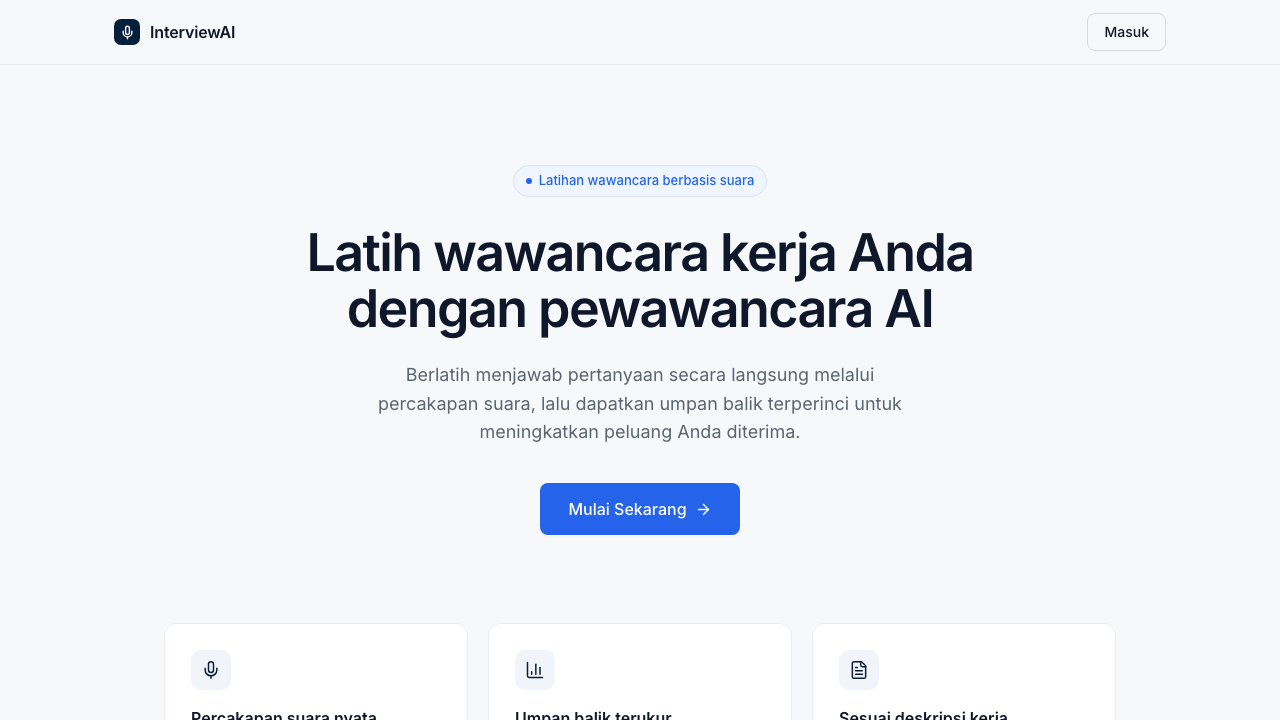
\includegraphics[width=\textwidth]{01-landing.png}
\caption{Halaman Landing}
\label{fig:landing}
\end{figure}

\begin{figure}[H]
\centering
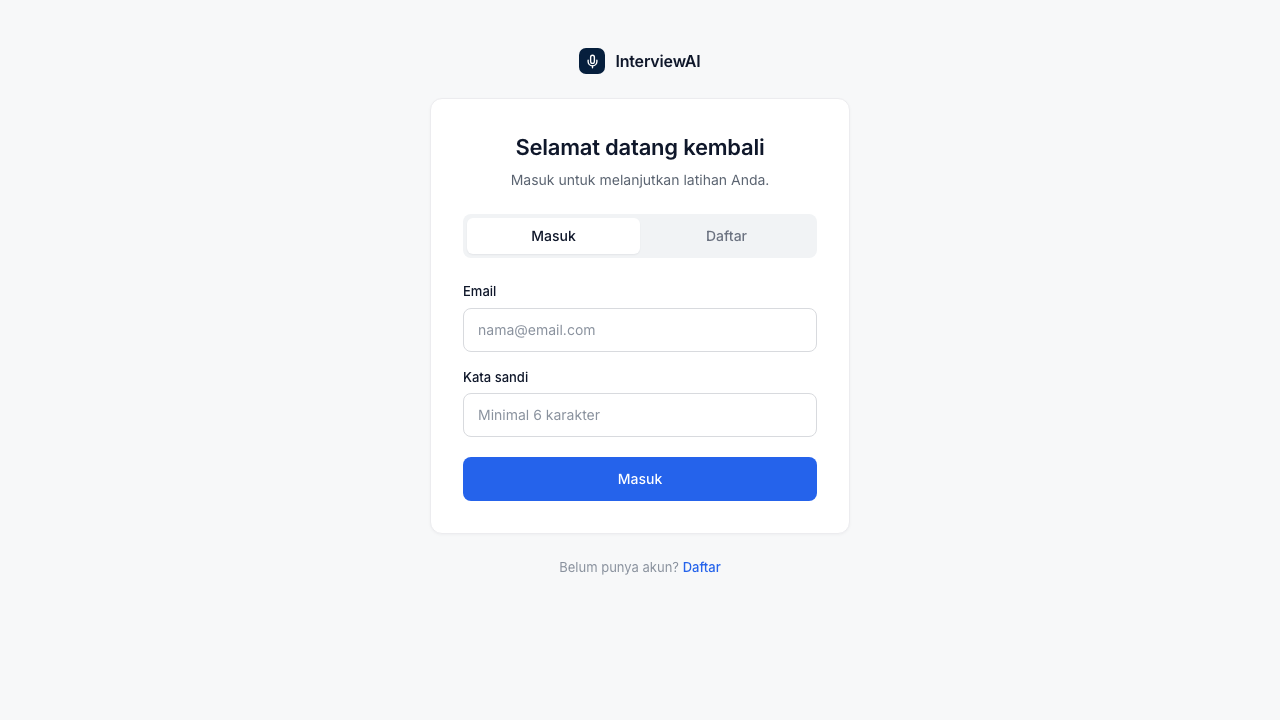
\includegraphics[width=0.8\textwidth]{02-login.png}
\caption{Halaman Login}
\label{fig:login}
\end{figure}

\begin{figure}[H]
\centering
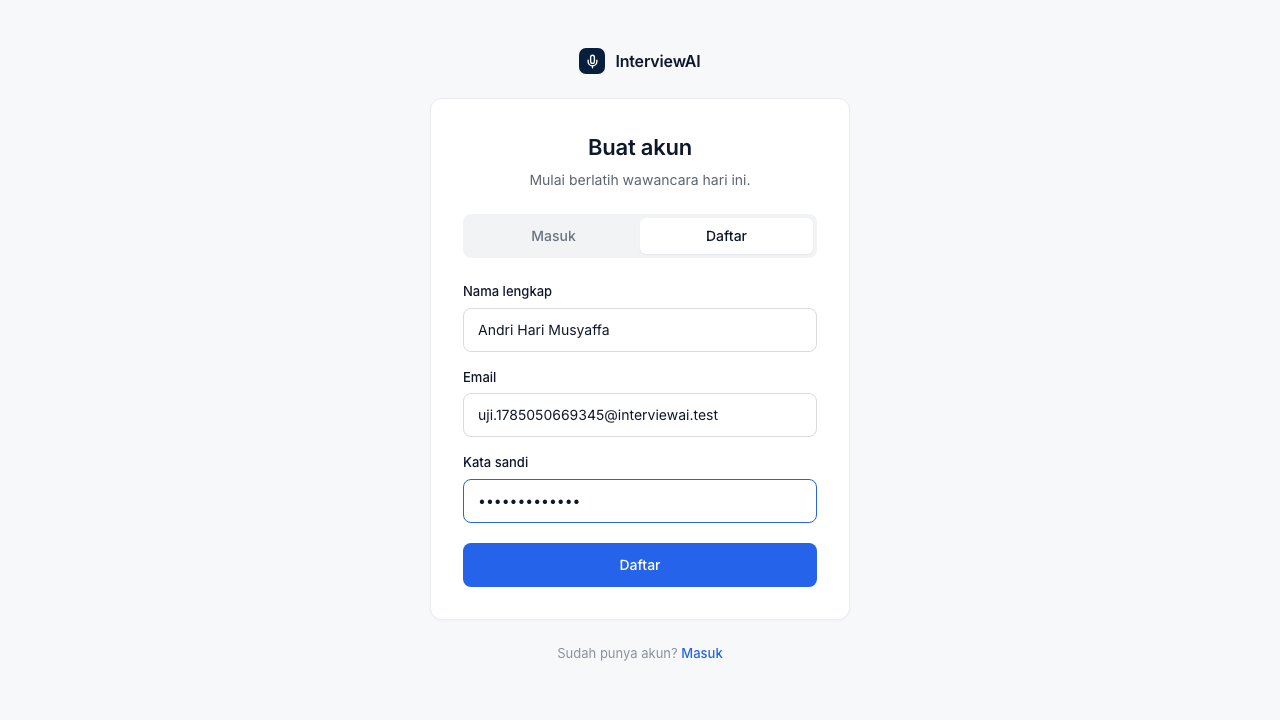
\includegraphics[width=0.8\textwidth]{03-register.png}
\caption{Halaman Register}
\label{fig:register}
\end{figure}

\begin{figure}[H]
\centering
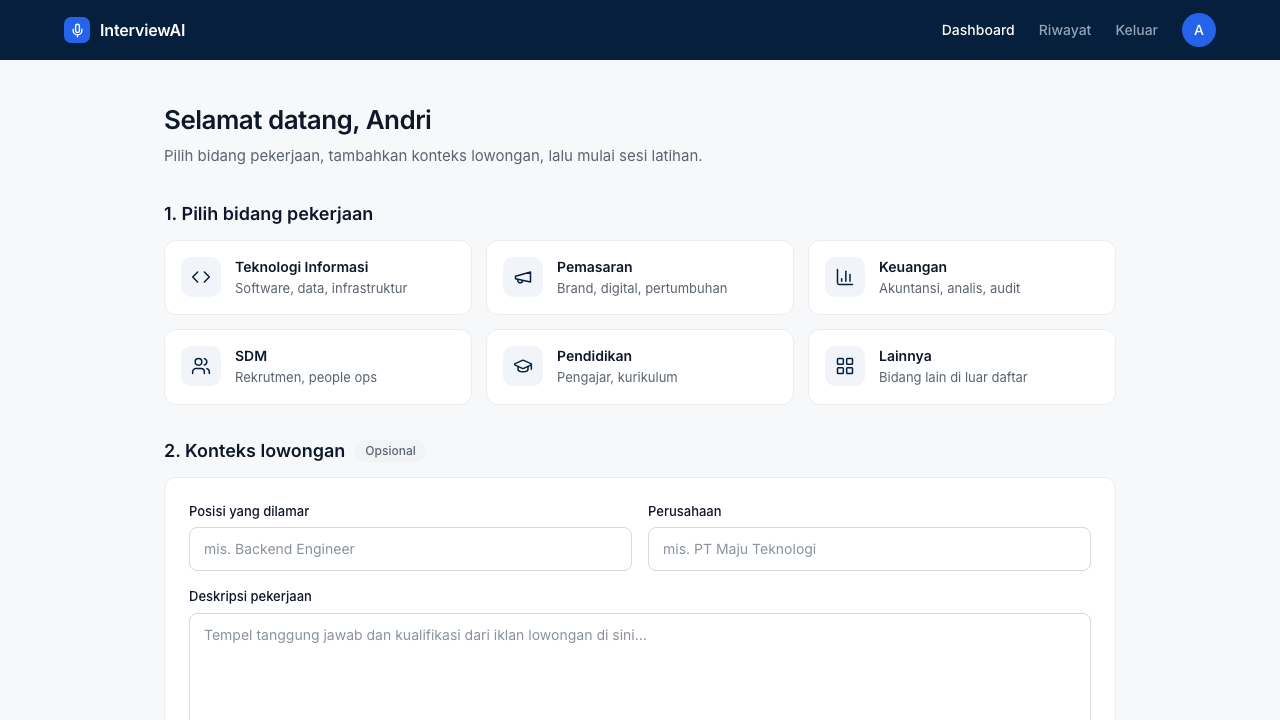
\includegraphics[width=\textwidth]{04-dashboard.png}
\caption{Halaman Dashboard --- Pemilihan Bidang Pekerjaan}
\label{fig:dashboard}
\end{figure}

\begin{figure}[H]
\centering
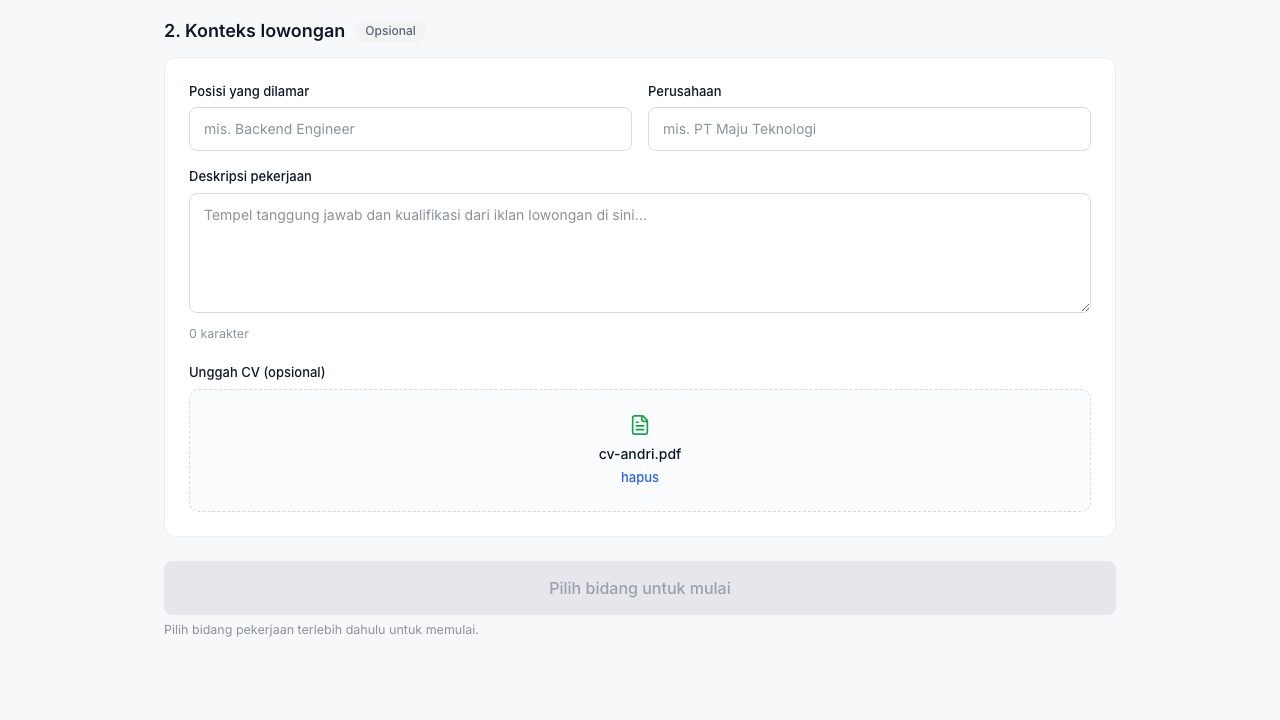
\includegraphics[width=\textwidth]{05-upload-cv.png}
\caption{Formulir Konteks Lowongan dan Unggah CV}
\label{fig:upload-cv}
\end{figure}

\begin{figure}[H]
\centering
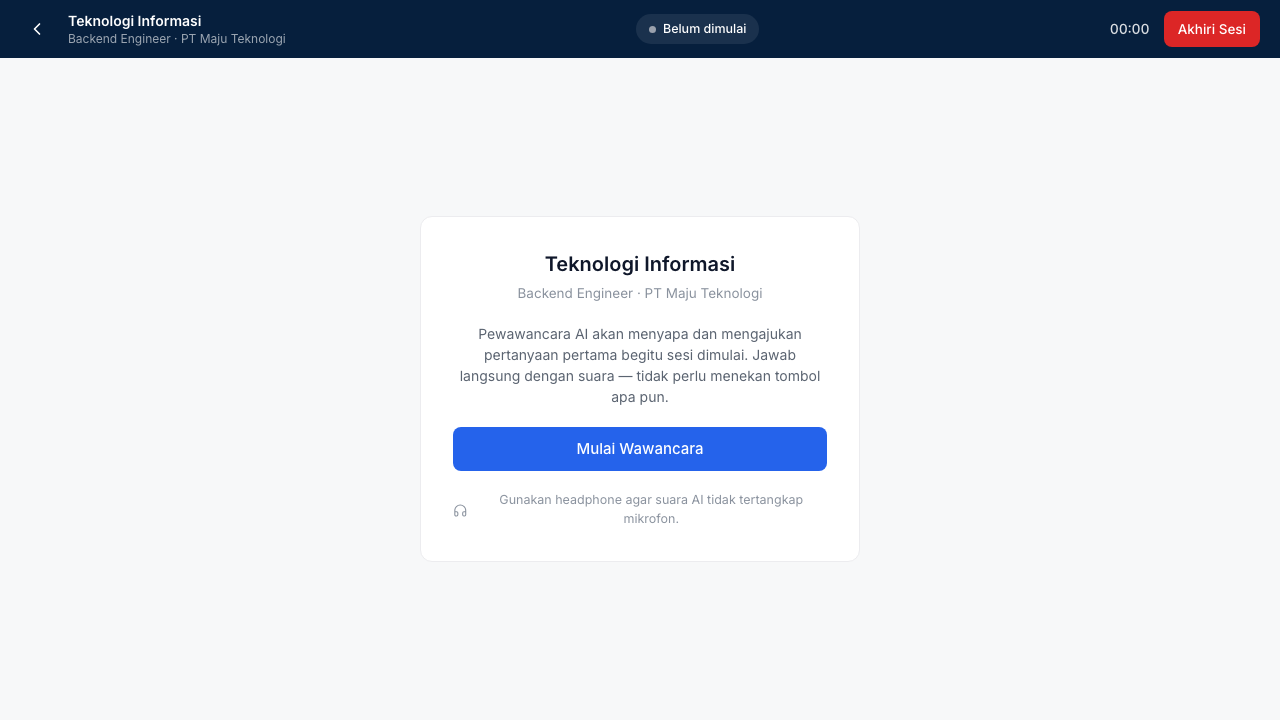
\includegraphics[width=\textwidth]{06-pre-session.png}
\caption{Halaman Persiapan Sesi Wawancara}
\label{fig:pre-session}
\end{figure}

\begin{figure}[H]
\centering
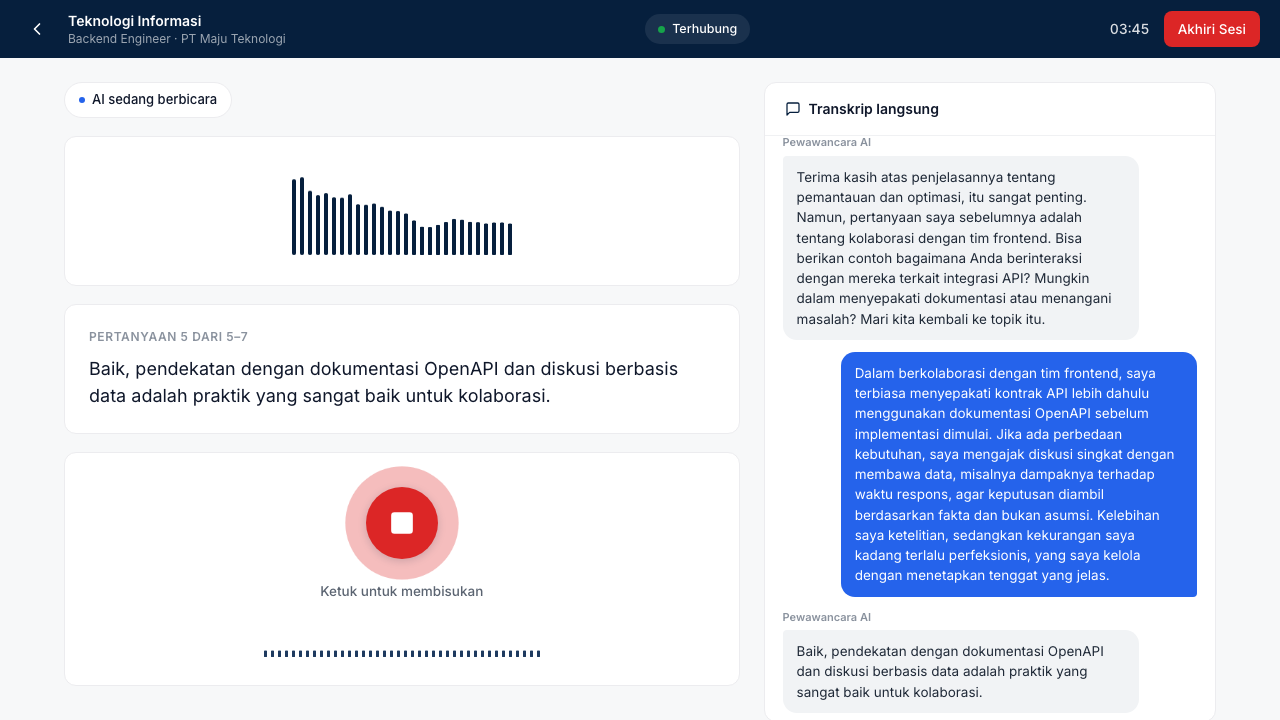
\includegraphics[width=\textwidth]{07-session-live.png}
\caption{Halaman Sesi Wawancara Berlangsung}
\label{fig:session-live}
\end{figure}

Gambar~\ref{fig:session-live} memperlihatkan sesi wawancara yang sedang
berjalan. Kolom kiri menampilkan indikator status pembicara, visualisasi
amplitudo audio, kartu pertanyaan terakhir, dan kendali mikrofon; sedangkan
kolom kanan menampilkan transkrip percakapan secara berurutan. Indikator
``Terhubung'' pada bilah atas menandakan koneksi \textit{WebSocket} ke Gemini
Live API dalam keadaan aktif, dan penghitung waktu menunjukkan durasi sesi
yang sedang berjalan.

\begin{figure}[H]
\centering
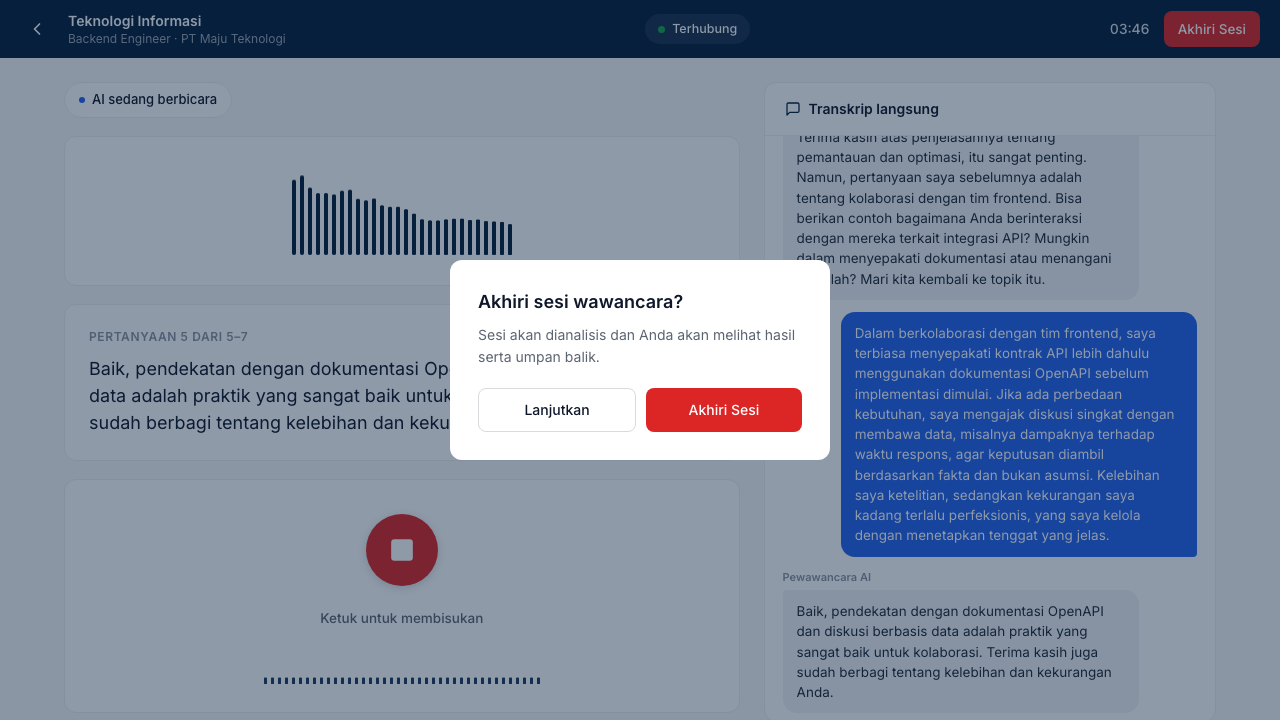
\includegraphics[width=\textwidth]{08-end-confirm.png}
\caption{Dialog Konfirmasi Pengakhiran Sesi}
\label{fig:end-confirm}
\end{figure}

\begin{figure}[H]
\centering
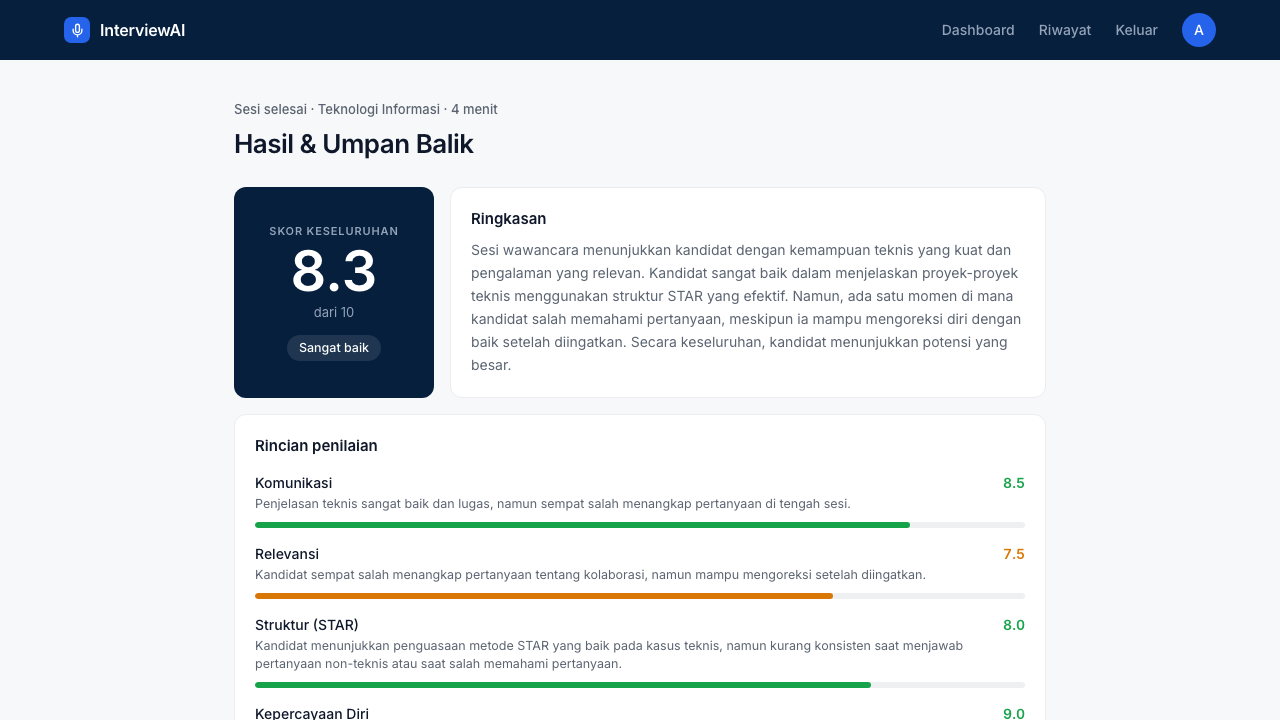
\includegraphics[width=\textwidth]{09-result.png}
\caption{Halaman Hasil dan Umpan Balik}
\label{fig:result}
\end{figure}

\begin{figure}[H]
\centering
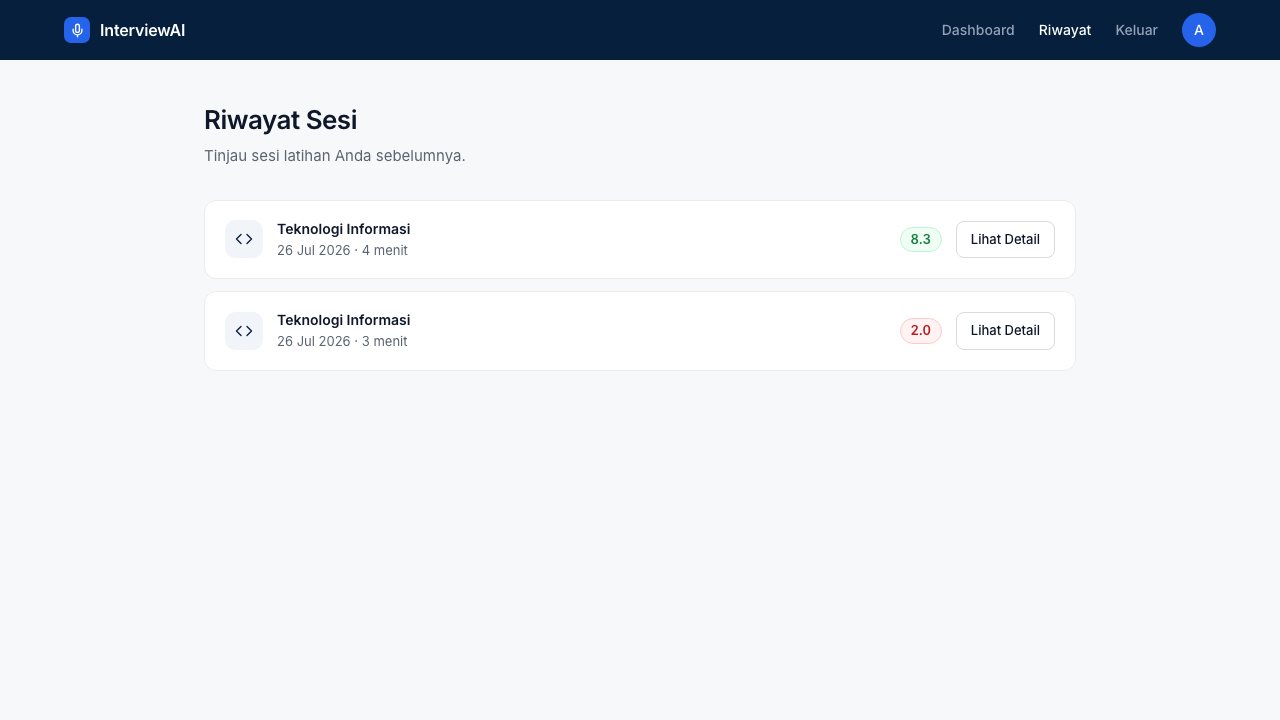
\includegraphics[width=\textwidth]{10-history.png}
\caption{Halaman Riwayat Sesi}
\label{fig:history}
\end{figure}

\begin{figure}[H]
\centering
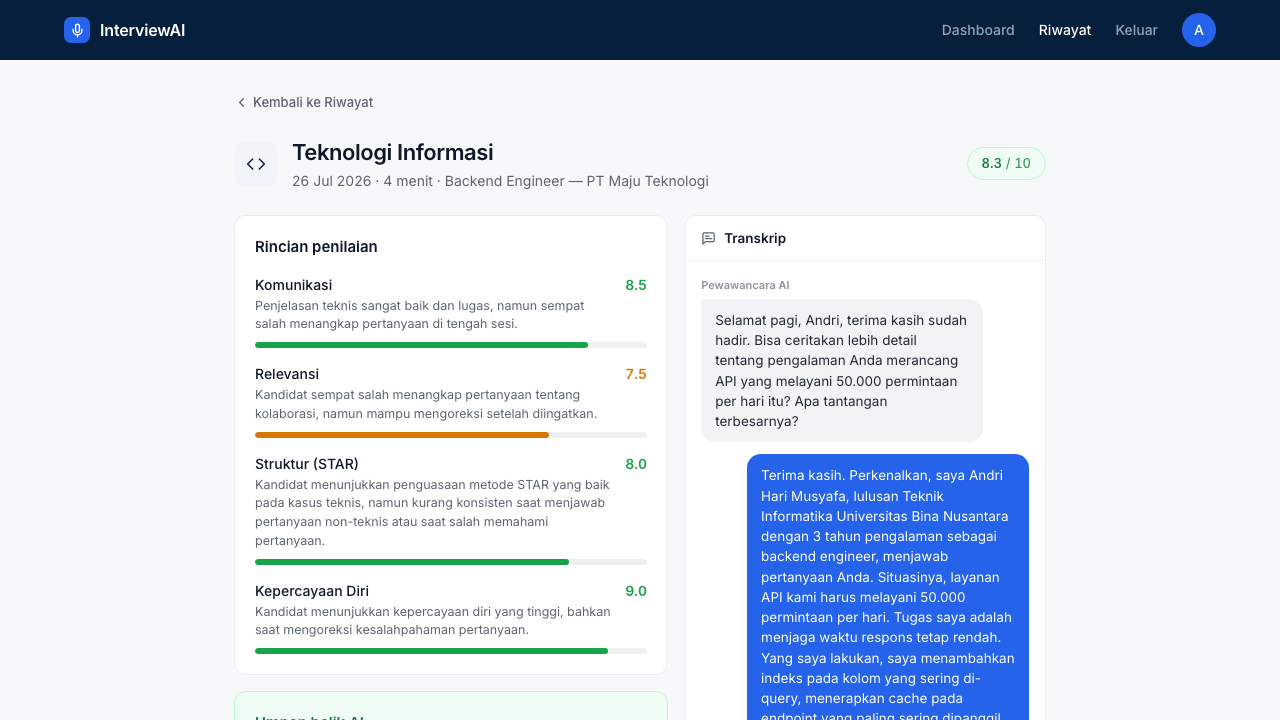
\includegraphics[width=\textwidth]{11-history-detail.png}
\caption{Halaman Detail Riwayat Sesi}
\label{fig:history-detail}
\end{figure}

\subsection{Implementasi Integrasi Gemini Live API}

Integrasi dengan Gemini Live API merupakan bagian paling kompleks dari sistem
ini karena melibatkan komunikasi audio dua arah secara \textit{real-time}.
Implementasinya menerapkan pola \textit{token broker}, yaitu \textit{backend}
tidak meneruskan aliran audio, melainkan hanya menerbitkan
\textit{ephemeral token} berumur pendek yang kemudian digunakan peramban untuk
membuka koneksi \textit{WebSocket Secure} langsung ke Gemini.

Alur satu sesi wawancara berjalan sebagai berikut:

\begin{enumerate}[leftmargin=*,itemsep=2pt]
  \item Pengguna memilih bidang pekerjaan, mengisi konteks lowongan, dan
        secara opsional mengunggah CV, lalu sistem membuat data sesi melalui
        \texttt{POST /api/sessions}.
  \item Peramban meminta \textit{ephemeral token} melalui
        \texttt{POST /api/sessions/:id/token}. Pada titik inilah
        \textit{backend} menyusun \textit{system instruction} yang berisi
        persona pewawancara beserta konteks sesi dan teks CV, lalu menguncinya
        di sisi server melalui \texttt{liveConnectConstraints}.
  \item Peramban membuka koneksi \textit{WebSocket} langsung ke Gemini
        menggunakan token tersebut, lalu mengirimkan perintah pembuka agar AI
        menyapa dan langsung mengajukan pertanyaan pertama.
  \item Audio mikrofon direkam pada 16 kHz, dikonversi menjadi PCM 16-bit di
        dalam \textit{AudioWorklet}, dan dikirimkan secara terus-menerus.
        Balasan audio Gemini pada 24 kHz diantrikan dan diputar kembali.
  \item Ketika pengguna mengakhiri sesi, transkrip dikirim ke
        \texttt{POST /api/sessions/}\linebreak[1]\texttt{:id/analyze} untuk dievaluasi, kemudian
        \texttt{POST /api/sessions/:id/end} menuliskan transkrip ke MongoDB
        lebih dahulu sebelum menandai sesi sebagai selesai di PostgreSQL.
\end{enumerate}

Parameter konfigurasi Gemini Live API hasil implementasi ditunjukkan pada
Tabel~\ref{tab:param-live}.

\begin{table}[H]
\caption{Parameter Konfigurasi Gemini Live API Hasil Implementasi}
\label{tab:param-live}
\centering
\begin{tabularx}{\textwidth}{|L{3.4cm}|L{4.2cm}|X|}
\hline
\textbf{Parameter} & \textbf{Nilai} & \textbf{Keterangan} \\
\hline
\textit{Model} & \texttt{gemini-3.1-flash-}\linebreak\texttt{live-preview} & Model \textit{native audio} dengan latensi terendah yang tersedia \\
\hline
Versi API & \texttt{v1alpha} & Versi yang menyediakan \textit{ephemeral token} \\
\hline
\textit{Response modalities} & \texttt{AUDIO} & Keluaran utama berupa audio \\
\hline
Transkripsi & \textit{input} dan \textit{output} diaktifkan & Menghasilkan transkrip dua arah untuk layar dan evaluasi \\
\hline
Format audio masuk & PCM 16-bit, 16 kHz, mono & Format yang diminta Gemini Live API \\
\hline
Format audio keluar & PCM 16-bit, 24 kHz, mono & Format balasan Gemini \\
\hline
\textit{Language code} & \texttt{id-ID} & Bahasa Indonesia \\
\hline
\textit{Voice} & \texttt{Kore} & Suara pewawancara AI \\
\hline
\textit{Temperature} & 0,7 & Keseimbangan variasi dan konsistensi respons \\
\hline
Masa berlaku token & 30 menit, sekali pakai & Membatasi dampak apabila token bocor \\
\hline
\end{tabularx}
\end{table}

\subsection{Implementasi Personalisasi Berbasis CV}

Berkas CV yang diunggah dalam format PDF maupun DOCX diekstraksi teksnya di
sisi \textit{backend}, lalu disisipkan ke dalam \textit{system instruction}
dengan batas maksimum 8.000 karakter. Pembatasan ini diperlukan karena
\textit{prompt} yang terlalu panjang meningkatkan biaya token sekaligus
latensi pada setiap sesi.

Efektivitas personalisasi ini terbukti pada saat pengujian. CV yang digunakan
memuat butir pengalaman berupa perancangan layanan API yang melayani 50.000
permintaan per hari. Pertanyaan pertama yang diajukan pewawancara AI adalah:

\begin{quote}
\textit{``Selamat pagi, Andri, terima kasih sudah hadir. Bisa ceritakan lebih
detail tentang pengalaman Anda merancang API yang melayani 50.000 permintaan
per hari itu? Apa tantangan terbesarnya?''}
\end{quote}

Pertanyaan tersebut menyebut angka yang hanya terdapat di dalam berkas CV,
sehingga membuktikan bahwa teks CV benar-benar terekstraksi, tersisipkan ke
dalam \textit{system instruction}, dan digunakan oleh model untuk menyusun
pertanyaan yang personal.

\subsection{Implementasi Evaluasi Terstruktur}

Evaluasi tidak dihasilkan oleh model percakapan, melainkan oleh model teks
terpisah (\texttt{gemini-2.5-flash}) yang menerima seluruh transkrip sesi.
Model diminta mengembalikan keluaran JSON terstruktur melalui mekanisme
\textit{response schema}, dengan empat metrik tetap yaitu Komunikasi,
Relevansi, Struktur (STAR), dan Kepercayaan Diri.

Karena keluaran model bahasa tetap berpotensi menyimpang dari skema yang
diminta, hasilnya melewati proses normalisasi sebelum disimpan. Proses ini
mencocokkan metrik berdasarkan \textit{key} maupun \textit{label},
membatasi setiap skor pada rentang 0--100, serta mengisi nilai cadangan
apabila ada bagian yang kosong. Dengan demikian bentuk data evaluasi yang
diterima antarmuka selalu konsisten, meskipun respons model bervariasi.

\subsection{Implementasi Keamanan}

Aspek keamanan yang berhasil diimplementasikan dirangkum pada
Tabel~\ref{tab:keamanan}.

\begin{table}[H]
\caption{Mekanisme Keamanan yang Diimplementasikan}
\label{tab:keamanan}
\centering
\begin{tabularx}{\textwidth}{|L{4.4cm}|X|}
\hline
\textbf{Aspek} & \textbf{Implementasi} \\
\hline
Kerahasiaan kunci API & Kunci API Gemini hanya berada di \textit{backend}; peramban hanya menerima \textit{ephemeral token} sekali pakai berumur 30 menit \\
\hline
Integritas persona AI & Model, \textit{system instruction}, suara, dan \textit{temperature} dikunci di sisi server; klien hanya boleh mengirim \textit{session resumption handle} \\
\hline
Autentikasi & JWT \textit{access token} berumur 15 menit dan \textit{refresh token} 7 hari pada \textit{cookie} \texttt{httpOnly} \\
\hline
Penyimpanan kata sandi & \textit{Hashing} menggunakan algoritma Argon2 \\
\hline
Pembatasan laju & 20 permintaan per IP tiap 15 menit pada \textit{endpoint} autentikasi, dan 40 permintaan per pengguna tiap 15 menit pada \textit{endpoint} yang memanggil Gemini \\
\hline
Otorisasi data & Setiap akses sesi maupun CV memverifikasi kepemilikan \texttt{user\_id}, dan parameter UUID divalidasi sebelum menyentuh basis data \\
\hline
Pengerasan HTTP & \textit{Helmet}, CORS dengan satu \textit{origin} dari variabel lingkungan, serta validasi variabel lingkungan saat proses \textit{boot} \\
\hline
\end{tabularx}
\end{table}

Pembatasan peran juga diterapkan pada tingkat \textit{prompt}. \textit{System
instruction} secara eksplisit melarang AI menjawab pertanyaan di luar konteks
wawancara serta mengabaikan permintaan untuk berganti peran atau membocorkan
isi instruksi, sebagai mitigasi terhadap upaya \textit{prompt injection}.

% =====================================================================
\section{Penyesuaian terhadap Rancangan BAB III}
% =====================================================================

Selama tahap implementasi ditemukan sejumlah kendala teknis yang menyebabkan
beberapa keputusan rancangan pada BAB III perlu disesuaikan. Ringkasan
penyesuaian tersebut ditunjukkan pada Tabel~\ref{tab:deviasi}, sedangkan
penyesuaian yang paling berdampak diuraikan pada sub-bab berikutnya.

\begin{table}[H]
\caption{Ringkasan Penyesuaian Rancangan terhadap Implementasi}
\label{tab:deviasi}
\centering
\begin{tabularx}{\textwidth}{|L{3.5cm}|L{3.4cm}|X|}
\hline
\textbf{Rancangan (BAB III)} & \textbf{Implementasi} & \textbf{Alasan Penyesuaian} \\
\hline
Supabase sebagai penyedia PostgreSQL, Auth, dan Storage & PostgreSQL mandiri, autentikasi JWT + Argon2 sendiri, CV disimpan pada \textit{filesystem} server & Menghilangkan ketergantungan pada layanan pihak ketiga dan biaya berlangganan, sekaligus memberi kendali penuh atas skema basis data dan masa berlaku token \\
\hline
\textit{Backend} berperan sebagai \textit{WebSocket proxy} & Pola \textit{token broker}; audio mengalir langsung dari peramban ke Gemini & \textit{Proxy} menambah satu lompatan jaringan pada jalur yang paling sensitif terhadap latensi dan membebani server dengan seluruh aliran audio. Pola \textit{token broker} tetap menjaga kerahasiaan kunci API tanpa biaya latensi tersebut \\
\hline
Model \texttt{gemini-live-}\linebreak\texttt{3-flash}, suara bawaan & \texttt{gemini-3.1-}\linebreak\texttt{flash-live-}\linebreak\texttt{preview}, suara \texttt{Kore}, \texttt{id-ID} & Nama model pada rancangan tidak tersedia. Model yang dipilih memberi waktu respons sekitar 1,5 detik dibanding sekitar 5,0 detik pada alternatifnya \\
\hline
Evaluasi berupa \texttt{overall\_score} dan \texttt{feedback\_text} & Ditambah empat metrik terstruktur, \texttt{strengths}, \texttt{improvements}, dan \texttt{summary} & Skor tunggal tidak cukup informatif sebagai bahan perbaikan. Penilaian per aspek menjawab kebutuhan umpan balik yang dapat ditindaklanjuti \\
\hline
Tipe kunci utama pada \texttt{job\_fields} adalah SERIAL & Bertipe UUID & Menyeragamkan tipe kunci seluruh tabel sehingga tidak ada identitas yang mudah ditebak berurutan \\
\hline
\textit{Deployment} pada Vercel dan Cloud Run & Direncanakan pada VPS di belakang \textit{nginx} & Menyederhanakan operasional menjadi satu lingkungan dan menekan biaya. Tahap ini belum dilaksanakan pada penelitian ini \\
\hline
\end{tabularx}
\end{table}

\subsection{Penggantian Supabase dengan Layanan Mandiri}

Rancangan awal menempatkan Supabase sebagai penyedia PostgreSQL, autentikasi,
dan penyimpanan berkas sekaligus. Pada implementasi, ketiga peran tersebut
dipisahkan dan dikelola sendiri. PostgreSQL dijalankan secara mandiri dengan
skema yang dikelola melalui berkas migrasi SQL berurutan, autentikasi
diimplementasikan menggunakan JWT dengan \textit{hashing} Argon2, dan berkas
CV disimpan pada \textit{filesystem} server dengan nama berkas yang diacak.

Konsekuensinya, pengelolaan keamanan autentikasi menjadi tanggung jawab
sistem ini sendiri. Hal tersebut dikompensasi dengan penerapan \textit{refresh
token} pada \textit{cookie} \texttt{httpOnly}, masa berlaku \textit{access
token} yang pendek, serta pembatasan laju pada \textit{endpoint}
autentikasi.

\subsection{Perubahan Pola Integrasi menjadi \textit{Token Broker}}

Perubahan paling mendasar terjadi pada pola integrasi dengan Gemini Live API.
Rancangan BAB III menempatkan \textit{backend} sebagai \textit{WebSocket
proxy} yang meneruskan audio dari klien ke Gemini. Pendekatan tersebut
memiliki dua kelemahan: seluruh aliran audio dua arah harus melewati server
sehingga menambah beban dan biaya bandwidth, dan setiap lompatan tambahan
menambah latensi pada jalur yang justru paling menentukan kealamian
percakapan.

Pada implementasi, \textit{backend} hanya berperan menerbitkan
\textit{ephemeral token}, sedangkan koneksi \textit{WebSocket} dibuka langsung
dari peramban ke Gemini. Kerahasiaan kunci API tetap terjaga karena kunci
tersebut tidak pernah meninggalkan server, dan konfigurasi sesi dikunci pada
saat token diterbitkan sehingga klien tidak dapat mengubah persona
pewawancara, model, maupun suara yang digunakan.

\subsection{Perluasan Skema Evaluasi}

Rancangan awal hanya menyimpan skor keseluruhan dan umpan balik naratif.
Skema tersebut diperluas menjadi empat metrik penilaian beserta catatannya,
ditambah daftar kelebihan, daftar hal yang perlu ditingkatkan, dan ringkasan
sesi. Perluasan ini menjawab tujuan penelitian mengenai umpan balik yang
bersifat personal, karena pengguna dapat mengetahui aspek mana yang lemah dan
bukan sekadar menerima satu angka.

% =====================================================================
\section{Pengujian Sistem}
% =====================================================================

\subsection{Metode dan Lingkungan Pengujian}

Pengujian dilakukan menggunakan metode \textit{Black Box Testing} sesuai
rencana pada BAB III, yaitu memvalidasi fungsionalitas berdasarkan masukan dan
keluaran yang diharapkan tanpa memeriksa struktur internal kode program.
Seluruh skenario diotomasi menggunakan Playwright dan dijalankan pada peramban
Chromium, sehingga pengujian dapat diulang dan hasilnya dapat diverifikasi
kembali.

Skenario dijalankan secara berurutan dalam satu \textit{worker} karena antar
skenario terdapat ketergantungan data: sesi wawancara yang diselesaikan pada
berkas skenario ketiga merupakan data yang diperiksa oleh skenario pengujian
riwayat. Dengan demikian alur simpan dan baca lintas kedua basis data ikut
terverifikasi.

Pengujian sesi wawancara suara memerlukan sumber suara kandidat. Suara
tersebut disintesis menggunakan \textit{text-to-speech} berbahasa Indonesia
berisi lima jawaban yang disusun mengikuti kerangka STAR, dengan jeda hening
di antara jawaban agar giliran bicara tidak bertabrakan dengan suara
pewawancara AI.

Pada tahap penyiapan ditemukan bahwa opsi Chromium
\texttt{-{}-use-file-for-}\allowbreak\texttt{fake-audio-capture} tidak berpengaruh pada
lingkungan pengujian yang digunakan. Hal ini diverifikasi menggunakan berkas
uji berpola nada keras dan hening bergantian setiap satu detik: pola tersebut
sama sekali tidak muncul pada data PCM yang benar-benar dikirimkan aplikasi ke
Gemini. Oleh karena itu mikrofon disimulasikan satu lapis lebih tinggi, yaitu
dengan mengembalikan \textit{MediaStream} yang dibangkitkan Web Audio API dari
berkas suara yang sama. Yang disimulasikan hanya perangkat keras mikrofonnya,
sedangkan seluruh jalur kode aplikasi --- \textit{AudioWorklet}, konversi PCM
16 kHz, hingga pengiriman ke Gemini --- tetap berjalan apa adanya, sehingga
pengujian tetap sah sebagai pengujian \textit{Black Box} terhadap sistem.

\subsection{Skenario dan Hasil Pengujian}

Sebanyak 26 skenario pengujian disusun untuk mencakup kesebelas
\textit{use case} yang dirancang pada BAB III, mencakup kasus normal maupun
kasus negatif. Hasil pengujian selengkapnya ditunjukkan pada
Tabel~\ref{tab:hasil-uji}.

\begin{longtable}{|C{1.1cm}|C{1.1cm}|L{4.5cm}|L{3.1cm}|C{1.3cm}|}
\caption{Hasil Pengujian \textit{Black Box}}
\label{tab:hasil-uji} \\
\hline
\textbf{Kode} & \textbf{UC} & \textbf{Skenario Pengujian} & \textbf{Hasil yang Diharapkan} & \textbf{Hasil} \\
\hline
\endfirsthead
\multicolumn{5}{l}{\small\textit{Lanjutan Tabel \ref{tab:hasil-uji}}} \\
\hline
\textbf{Kode} & \textbf{UC} & \textbf{Skenario Pengujian} & \textbf{Hasil yang Diharapkan} & \textbf{Hasil} \\
\hline
\endhead
\hline
\endfoot
\hline
\endlastfoot

TC-00 & -- & Membuka halaman Landing & Judul dan tombol ``Mulai Sekarang'' tampil & Valid \\
\hline
TC-01 & UC-02 & Membuka Dashboard tanpa autentikasi & Dialihkan ke halaman Login & Valid \\
\hline
TC-02 & UC-01 & Register dengan format email tidak valid & Pesan ``Masukkan email yang valid'' tampil & Valid \\
\hline
TC-03 & UC-01 & Register dengan kata sandi kurang dari 6 karakter & Pesan ``Kata sandi minimal 6 karakter'' tampil & Valid \\
\hline
TC-04 & UC-01 & Register dengan data lengkap dan valid & Akun terbentuk dan masuk ke Dashboard & Valid \\
\hline
TC-05 & UC-01 & Register dengan email yang sudah terdaftar & Ditolak server dengan pesan galat & Valid \\
\hline
TC-06 & UC-02 & Login dengan kata sandi salah & Ditolak dan tetap di halaman Login & Valid \\
\hline
TC-07 & UC-02 & Login dengan kredensial benar & Masuk ke Dashboard & Valid \\
\hline
TC-08 & UC-10 & Menekan tombol Keluar & Sesi berakhir dan halaman terproteksi diblokir & Valid \\
\hline
TC-09 & UC-03 & Memuat daftar bidang pekerjaan & Enam bidang pekerjaan tampil dari server & Valid \\
\hline
TC-10 & UC-03 & Belum memilih bidang pekerjaan & Tombol mulai sesi dalam keadaan nonaktif & Valid \\
\hline
TC-11 & UC-03 & Memilih salah satu bidang pekerjaan & Tombol mulai sesi menjadi aktif & Valid \\
\hline
TC-12 & UC-03 & Mengisi deskripsi lowongan lebih dari 40 karakter & Konfirmasi ``Konteks akan dipakai AI'' tampil & Valid \\
\hline
TC-13 & UC-11 & Mengunggah CV berformat PDF & Berkas terunggah dan teksnya terekstraksi & Valid \\
\hline
TC-14 & UC-11 & Mengunggah CV berformat DOCX & Berkas terunggah dan teksnya terekstraksi & Valid \\
\hline
TC-15 & UC-11 & Mengunggah berkas berformat selain PDF/DOCX & Ditolak dengan pesan format tidak sesuai & Valid \\
\hline
TC-16 & UC-11 & Menghapus CV yang telah diunggah & Formulir kembali ke keadaan semula & Valid \\
\hline
TC-17 & UC-04 & Menekan tombol Mulai Sesi Wawancara & Sesi terbentuk dan halaman wawancara terbuka & Valid \\
\hline
TC-18 & UC-04 & Memulai wawancara & Koneksi terbuka dan AI menyapa serta bertanya & Valid \\
\hline
TC-19 & UC-05 & Kandidat menjawab dengan suara & Jawaban tertranskripsi pada panel transkrip & Valid \\
\hline
TC-20 & UC-06 & Melanjutkan percakapan beberapa giliran & AI menanggapi jawaban dan mengajukan pertanyaan lanjutan & Valid \\
\hline
TC-21 & UC-07 & Mengakhiri sesi wawancara & Evaluasi dihasilkan dan halaman Hasil tampil lengkap & Valid \\
\hline
TC-22 & UC-08 & Membuka halaman Riwayat & Sesi yang telah selesai tampil beserta skornya & Valid \\
\hline
TC-23 & UC-09 & Membuka detail salah satu sesi & Rincian penilaian dan transkrip tampil & Valid \\
\hline
TC-24 & UC-09 & Membuka detail sesi milik pengguna lain & Akses ditolak dan pesan galat tampil & Valid \\
\hline
TC-25 & UC-09 & Kembali dari detail ke daftar riwayat & Kembali ke halaman Riwayat & Valid \\
\hline
\end{longtable}

\subsection{Analisis Persentase Keberhasilan}

Persentase keberhasilan dihitung menggunakan rumus yang telah ditetapkan pada
BAB III, yaitu:

\begin{center}
\textit{Success Rate} $=\dfrac{\text{Jumlah \textit{test case} valid}}{\text{Total \textit{test case}}}\times 100\%$
\end{center}

Rekapitulasi hasil pengujian per \textit{use case} ditunjukkan pada
Tabel~\ref{tab:success-rate}.

\begin{table}[H]
\caption{Rekapitulasi Persentase Keberhasilan per \textit{Use Case}}
\label{tab:success-rate}
\centering
\begin{tabularx}{\textwidth}{|C{1.6cm}|X|C{1.9cm}|C{1.6cm}|C{2.1cm}|}
\hline
\textbf{Kode UC} & \textbf{Nama \textit{Use Case}} & \textbf{Jumlah \textit{Test Case}} & \textbf{Valid} & \textbf{Persentase} \\
\hline
UC-01 & Register & 4 & 4 & 100\% \\
\hline
UC-02 & Login & 3 & 3 & 100\% \\
\hline
UC-03 & Memilih Bidang Pekerjaan & 4 & 4 & 100\% \\
\hline
UC-04 & Memulai Sesi Wawancara & 2 & 2 & 100\% \\
\hline
UC-05 & Menjawab Pertanyaan & 1 & 1 & 100\% \\
\hline
UC-06 & Menerima Umpan Balik & 1 & 1 & 100\% \\
\hline
UC-07 & Mengakhiri Sesi & 1 & 1 & 100\% \\
\hline
UC-08 & Melihat Riwayat Sesi & 1 & 1 & 100\% \\
\hline
UC-09 & Melihat Detail Riwayat & 3 & 3 & 100\% \\
\hline
UC-10 & Logout & 1 & 1 & 100\% \\
\hline
UC-11 & Mengunggah CV & 4 & 4 & 100\% \\
\hline
-- & Umum (halaman Landing) & 1 & 1 & 100\% \\
\hline
\multicolumn{2}{|c|}{\textbf{Total}} & \textbf{26} & \textbf{26} & \textbf{100\%} \\
\hline
\end{tabularx}
\end{table}

Berdasarkan rekapitulasi tersebut, seluruh 26 \textit{test case} dinyatakan
valid sehingga persentase keberhasilan mencapai 100\%. Nilai ini melampaui
ambang minimal 90\% untuk setiap kategori fitur yang ditetapkan pada BAB III,
sehingga hipotesis penelitian mengenai keberhasilan fungsional sistem
dinyatakan terpenuhi.

% =====================================================================
\section{Pembahasan}
% =====================================================================

\subsection{Ketercapaian Tujuan Penelitian}

Rumusan masalah pertama mempertanyakan bagaimana merancang dan membangun
\textit{website} simulasi wawancara kerja berbasis \textit{Large Language
Model} dengan memanfaatkan Gemini Live API. Hasil implementasi menunjukkan
bahwa sistem tersebut berhasil dibangun secara utuh, mulai dari autentikasi,
konfigurasi sesi, wawancara suara \textit{real-time}, evaluasi otomatis,
hingga riwayat sesi. Sistem berjalan sepenuhnya di dalam peramban tanpa
memerlukan pemasangan perangkat lunak tambahan, dan seluruh antarmukanya
menggunakan Bahasa Indonesia sehingga dapat diakses oleh pencari kerja di
Indonesia tanpa hambatan bahasa maupun biaya sesi.

Rumusan masalah kedua mempertanyakan bagaimana mengintegrasikan fitur
pertanyaan otomatis, penilaian jawaban, umpan balik personal, dan komunikasi
suara \textit{real-time} ke dalam satu \textit{platform} berbasis web.
Keempat fitur tersebut terbukti berjalan dalam satu alur yang berkesinambungan
sebagaimana ditunjukkan pada pengujian TC-17 sampai TC-21. Pertanyaan
dihasilkan secara otomatis dan dipersonalisasi berdasarkan CV, jawaban
disampaikan melalui suara dan tertranskripsi, umpan balik lisan diberikan di
sela percakapan, serta penilaian tertulis per aspek disajikan setelah sesi
berakhir.

\subsection{Analisis Kinerja Percakapan \textit{Real-time}}

Pengukuran kinerja diambil langsung pada saat pengujian sesi wawancara
berlangsung dan dirangkum pada Tabel~\ref{tab:kinerja}.

\begin{table}[H]
\caption{Hasil Pengukuran Kinerja Sesi Wawancara}
\label{tab:kinerja}
\centering
\begin{tabularx}{\textwidth}{|X|C{3cm}|}
\hline
\textbf{Aspek yang Diukur} & \textbf{Hasil} \\
\hline
Waktu dari penekanan tombol mulai hingga AI mengucapkan sapaan pertama & 2,2 detik \\
\hline
Waktu dari mulai berbicara hingga jawaban muncul pada panel transkrip & 58,1 detik\footnotemark \\
\hline
Jumlah giliran bicara pewawancara AI dalam satu sesi & 5 giliran \\
\hline
Jumlah giliran bicara kandidat dalam satu sesi & 4 giliran \\
\hline
Total panjang transkrip jawaban kandidat & 1.856 karakter \\
\hline
Waktu pembuatan evaluasi setelah sesi diakhiri & 11,9 detik \\
\hline
\end{tabularx}
\end{table}
\footnotetext{Angka ini mencakup jeda hening 17 detik pada awal berkas suara
uji dan durasi pengucapan jawaban itu sendiri, sehingga bukan merupakan
latensi transkripsi murni. Latensi transkripsi terukur berada pada kisaran 3
detik di belakang penutur.}

Waktu tanggap awal sebesar 2,2 detik menunjukkan bahwa pola \textit{token
broker} tidak menimbulkan penundaan yang terasa, meskipun peramban harus
meminta token ke \textit{backend} terlebih dahulu sebelum membuka koneksi ke
Gemini. Adapun waktu pembuatan evaluasi sebesar 11,9 detik masih dapat
diterima karena berlangsung sekali di akhir sesi dan disertai indikator
pemuatan pada antarmuka.

Karakteristik penting yang ditemukan pada tahap implementasi adalah bahwa
transkripsi masukan dari Gemini berjalan sekitar tiga detik di belakang
penutur. Akibatnya, indikator ``sedang berbicara'' pada antarmuka tidak dapat
mengandalkan transkrip tersebut. Sistem mengatasinya dengan mendeteksi
amplitudo suara secara lokal di peramban, dan sinyal tersebut digunakan
semata-mata untuk keperluan tampilan, tidak pernah untuk menggerbang
pengiriman audio ke Gemini.

\subsection{Analisis Kualitas Evaluasi}

Selama tahap pengujian dilakukan dua kali sesi wawancara dengan naskah jawaban
yang berbeda, dan perbandingan hasilnya ditunjukkan pada
Tabel~\ref{tab:banding-evaluasi}.

\begin{table}[H]
\caption{Perbandingan Hasil Evaluasi terhadap Dua Naskah Jawaban}
\label{tab:banding-evaluasi}
\centering
\begin{tabularx}{\textwidth}{|X|C{2.4cm}|C{2.4cm}|}
\hline
\textbf{Karakteristik Naskah Jawaban} & \textbf{Skor Keseluruhan} & \textbf{Skor Relevansi} \\
\hline
Jawaban umum yang tidak menanggapi pertanyaan spesifik pewawancara & 2,0 & 1,5 \\
\hline
Jawaban terstruktur STAR yang menanggapi pokok pertanyaan & 8,3 & tinggi \\
\hline
\end{tabularx}
\end{table}

Perbedaan skor yang lebar antara kedua naskah menunjukkan bahwa mekanisme
evaluasi bersifat diskriminatif, yaitu benar-benar menilai isi dan relevansi
jawaban dan bukan sekadar memberikan skor tinggi secara seragam. Pada naskah
pertama, sistem secara tepat mengidentifikasi bahwa kandidat berulang kali
tidak menjawab pertanyaan yang diajukan, dan hal tersebut tercermin pada skor
Relevansi yang rendah. Temuan ini memperkuat keyakinan bahwa umpan balik yang
dihasilkan sistem memiliki nilai diagnostik bagi pengguna.

\subsection{Keterbatasan Sistem}

Berdasarkan hasil implementasi dan pengujian, terdapat sejumlah keterbatasan
yang perlu dicatat:

\begin{enumerate}[leftmargin=*,itemsep=3pt]
  \item \textbf{Ketergantungan pada model \textit{preview}.} Model
        \texttt{gemini-3.1-flash-}\allowbreak\texttt{live-preview} berstatus
        \textit{preview}
        sehingga berpotensi berubah atau dihentikan sewaktu-waktu. Sistem
        belum memiliki mekanisme peralihan otomatis ke model cadangan.
  \item \textbf{Penentuan batas giliran bicara bersifat heuristik.} Karena
        Gemini tidak menyertakan penanda waktu pengucapan pada setiap potongan
        transkrip, sistem menentukan giliran berdasarkan waktu kedatangan
        data. Pada kondisi tertentu, beberapa kata terakhir sebuah jawaban
        dapat tergeser ke giliran berikutnya, meskipun isi dan urutan
        percakapan secara keseluruhan tetap terjaga.
  \item \textbf{Penilaian terbatas pada aspek verbal.} Sesuai ruang lingkup
        pada BAB III, sistem tidak menilai aspek psikologis maupun bahasa
        tubuh, karena masukannya hanya berupa suara.
  \item \textbf{Pengujian belum mencakup keberagaman pengguna nyata.}
        Pengujian dilakukan menggunakan suara sintetis pada satu lingkungan
        peramban. Variasi aksen, kecepatan bicara, kualitas mikrofon, dan
        kondisi kebisingan pengguna nyata belum terwakili.
  \item \textbf{Tahap \textit{deployment} belum dilaksanakan.} Sistem baru
        berjalan pada lingkungan pengembangan lokal, sehingga pengujian
        performa pada kondisi produksi belum dapat dilakukan.
\end{enumerate}

\end{document}
. Bila
% disisipkan, preamble di bawah diabaikan secara otomatis.
% =====================================================================
\documentclass[12pt,a4paper,oneside]{report}

\usepackage[T1]{fontenc}
\usepackage[utf8]{inputenc}
\usepackage{newtxtext,newtxmath}          % Times New Roman
\usepackage[bahasa]{babel}
\usepackage[a4paper,left=4cm,right=3cm,top=3cm,bottom=3cm]{geometry}
\usepackage{setspace}
\usepackage{graphicx}
\usepackage{array}
\usepackage{longtable}
\usepackage{tabularx}
\usepackage{ragged2e}
\usepackage{enumitem}
\usepackage{caption}
\usepackage{float}
\usepackage{titlesec}
\usepackage[hidelinks]{hyperref}

% Judul bab bergaya skripsi: "BAB IV" di atas, judul bab di bawahnya, keduanya
% rata tengah dan huruf kapital.
\titleformat{\chapter}[display]
  {\normalfont\bfseries\centering}
  {\Large BAB \Roman{chapter}}{12pt}{\Large}
\titlespacing*{\chapter}{0pt}{0pt}{28pt}

\graphicspath{{gambar/}}

% Judul tabel di atas, judul gambar di bawah, keduanya rata tengah dan tebal.
\captionsetup[table]{position=top,labelsep=space,font=bf,justification=centering}
\captionsetup[figure]{position=bottom,labelsep=space,font=bf,justification=centering}

\newcolumntype{L}[1]{>{\RaggedRight\arraybackslash}p{#1}}
\newcolumntype{C}[1]{>{\Centering\arraybackslash}p{#1}}

\setlength{\emergencystretch}{3em}

\setcounter{chapter}{3}   % bab berikutnya menjadi BAB IV
\onehalfspacing

\begin{document}

\chapter{HASIL DAN PEMBAHASAN}

Bab ini menyajikan hasil tahap implementasi dan tahap pengujian dari metode
pengembangan \textit{Waterfall} yang telah diuraikan pada BAB III. Pembahasan
dimulai dari lingkungan implementasi dan wujud sistem yang berhasil dibangun,
dilanjutkan dengan penjelasan mengenai penyesuaian yang dilakukan terhadap
rancangan awal beserta alasan teknisnya, kemudian hasil pengujian
\textit{Black Box} atas seluruh \textit{use case}, dan ditutup dengan
pembahasan mengenai ketercapaian tujuan penelitian serta keterbatasan sistem.

% =====================================================================
\section{Lingkungan Implementasi}
% =====================================================================

Sistem dibangun dan diuji pada lingkungan pengembangan dengan spesifikasi
sebagaimana ditunjukkan pada Tabel~\ref{tab:lingkungan}. Seluruh komponen
dijalankan secara lokal, kecuali layanan Gemini yang diakses melalui jaringan
internet.

\begin{table}[H]
\caption{Spesifikasi Lingkungan Implementasi dan Pengujian}
\label{tab:lingkungan}
\centering
\begin{tabularx}{\textwidth}{|L{4cm}|X|}
\hline
\textbf{Komponen} & \textbf{Spesifikasi} \\
\hline
Sistem operasi & macOS (Darwin 25.5.0), arsitektur ARM64 \\
\hline
\textit{Runtime} & Node.js v25.4.0, npm \textit{workspaces} \\
\hline
Basis data relasional & PostgreSQL 18.3 \\
\hline
Basis data dokumen & MongoDB 7.0.39 (kontainer Docker) \\
\hline
Peramban pengujian & Chromium (Playwright 1.62) \\
\hline
Layanan AI percakapan & Gemini Live API, model \texttt{gemini-3.1-flash-live-preview} \\
\hline
Layanan AI evaluasi & Gemini API, model \texttt{gemini-2.5-flash} \\
\hline
Alamat aplikasi & \textit{Frontend} \texttt{localhost:5180}, \textit{backend} \texttt{localhost:4000} \\
\hline
\end{tabularx}
\end{table}

Pustaka utama yang digunakan pada masing-masing lapisan ditunjukkan pada
Tabel~\ref{tab:pustaka}.

\begin{table}[H]
\caption{Pustaka Utama yang Digunakan}
\label{tab:pustaka}
\centering
\begin{tabularx}{\textwidth}{|L{3cm}|L{4.6cm}|X|}
\hline
\textbf{Lapisan} & \textbf{Pustaka} & \textbf{Fungsi} \\
\hline
\textit{Frontend} & React 18.3, Vite 6.4, TypeScript 5.7, Tailwind CSS 4.0, React Router 7.1 & Antarmuka pengguna, \textit{routing}, dan gaya visual \\
\hline
\textit{Frontend} & \texttt{@google/genai} 2.11 & Klien Gemini Live API di sisi peramban \\
\hline
\textit{Backend} & Express 4.21, TypeScript 5.7 & Kerangka REST API \\
\hline
\textit{Backend} & \texttt{pg} 8.13, \texttt{mongodb} 7.5 & Akses PostgreSQL dan MongoDB \\
\hline
\textit{Backend} & \texttt{jsonwebtoken} 9.0, \texttt{@node-rs/argon2} 2.0 & Autentikasi JWT dan \textit{hashing} kata sandi \\
\hline
\textit{Backend} & \texttt{zod} 3.24, \texttt{helmet} 8.0, \texttt{express-rate-limit} 7.5 & Validasi masukan, pengerasan HTTP, pembatasan laju \\
\hline
\textit{Backend} & \texttt{multer} 2.2, \texttt{pdf-parse} 2.4, \texttt{mammoth} 1.12 & Unggah berkas CV dan ekstraksi teks PDF/DOCX \\
\hline
Pengujian & \texttt{@playwright/test} 1.62 & Otomasi pengujian \textit{Black Box} \\
\hline
\end{tabularx}
\end{table}

% =====================================================================
\section{Hasil Implementasi Sistem}
% =====================================================================

\subsection{Struktur Kode Program}

Sistem diimplementasikan sebagai \textit{monorepo} dengan npm
\textit{workspaces} yang terdiri atas dua paket, yaitu \texttt{frontend/} dan
\texttt{backend/}. Pemisahan ini menjaga agar kedua sisi memiliki
\textit{dependency} dan konfigurasi TypeScript sendiri, namun tetap dapat
dijalankan bersama melalui satu perintah. Struktur direktori inti ditunjukkan
pada Tabel~\ref{tab:struktur}.

\begin{table}[H]
\caption{Struktur Direktori Inti Sistem}
\label{tab:struktur}
\centering
\begin{tabularx}{\textwidth}{|L{5.6cm}|X|}
\hline
\textbf{Direktori} & \textbf{Isi} \\
\hline
\texttt{backend/src/config} & Validasi variabel lingkungan, \textit{pool} PostgreSQL, klien MongoDB \\
\hline
\texttt{backend/src/db/migrations} & Enam berkas migrasi SQL berurutan beserta data \textit{seed} \\
\hline
\texttt{backend/src/middleware} & \texttt{requireAuth}, pembatas laju, penanganan galat terpusat \\
\hline
\texttt{backend/src/modules} & Modul per domain: \texttt{auth}, \texttt{jobFields}, \texttt{sessions}, \texttt{cv}, \texttt{gemini} \\
\hline
\texttt{frontend/src/pages} & Tujuh halaman: Landing, Login, Dashboard, Session, Result, History, HistoryDetail \\
\hline
\texttt{frontend/src/features/}\linebreak\texttt{session} & Komponen layar wawancara langsung \\
\hline
\texttt{frontend/src/lib/audio} & Perekaman mikrofon 16 kHz, pemutaran 24 kHz, konversi PCM \\
\hline
\texttt{frontend/src/lib/gemini} & \texttt{liveClient} sebagai pembungkus Gemini Live API \\
\hline
\texttt{tests/e2e} & Skenario pengujian \textit{Black Box} otomatis \\
\hline
\end{tabularx}
\end{table}

Setiap modul \textit{backend} disusun mengikuti pola berlapis
\textit{routes} $\rightarrow$ \textit{controller} $\rightarrow$
\textit{service}, dengan skema Zod terpisah untuk validasi masukan. Pola ini
menjaga agar logika bisnis tidak bercampur dengan penanganan HTTP, sehingga
tiap lapisan dapat dipahami dan diubah secara mandiri.

\subsection{Implementasi Basis Data}

Basis data relasional diimplementasikan pada PostgreSQL melalui enam berkas
migrasi SQL yang dijalankan berurutan. Terdapat lima tabel sebagaimana
dirancang pada BAB III, yaitu \texttt{users}, \texttt{job\_fields},
\texttt{interview\_sessions}, \texttt{evaluations}, dan
\texttt{cv\_documents}. Transkrip percakapan disimpan pada MongoDB dalam
koleksi \texttt{transcripts}.

Realisasi struktur tabel memiliki beberapa perbedaan terhadap rancangan awal,
terutama pada tabel \texttt{evaluations} yang diperluas untuk menampung hasil
penilaian terstruktur. Kamus data hasil implementasi untuk tabel tersebut
ditunjukkan pada Tabel~\ref{tab:kamus-evaluations}.

\begin{table}[H]
\caption{Kamus Data Tabel \texttt{evaluations} Hasil Implementasi}
\label{tab:kamus-evaluations}
\centering
\begin{tabularx}{\textwidth}{|L{3cm}|L{3cm}|L{1.6cm}|X|}
\hline
\textbf{Nama Field} & \textbf{Tipe Data} & \textbf{Kunci} & \textbf{Keterangan} \\
\hline
\texttt{id} & UUID & PK & Identitas unik evaluasi \\
\hline
\texttt{session\_id} & UUID & FK, UNIQUE & Referensi ke \texttt{interview\_sessions.id}; relasi satu ke satu \\
\hline
\texttt{overall\_score} & INTEGER & -- & Skor keseluruhan, dibatasi rentang 0--100 \\
\hline
\texttt{feedback\_text} & TEXT & -- & Umpan balik naratif dari AI \\
\hline
\texttt{metrics} & JSONB & -- & Empat metrik penilaian beserta skor dan catatannya \\
\hline
\texttt{strengths} & JSONB & -- & Daftar poin ``yang sudah baik'' \\
\hline
\texttt{improvements} & JSONB & -- & Daftar poin ``bisa ditingkatkan'' \\
\hline
\texttt{summary} & TEXT & -- & Ringkasan naratif sesi \\
\hline
\texttt{created\_at} & TIMESTAMPTZ & -- & Waktu evaluasi dibuat \\
\hline
\end{tabularx}
\end{table}

Integritas data dijaga melalui \textit{constraint} pada tingkat basis data,
yaitu \textit{foreign key} \texttt{user\_id} dengan aksi
\texttt{ON DELETE CASCADE}, \textit{foreign key} \texttt{cv\_id} yang
bersifat \textit{nullable} dengan aksi \texttt{ON DELETE SET NULL} sesuai
sifat opsional fitur unggah CV, serta \textit{check constraint} yang membatasi
nilai \texttt{status} hanya pada \texttt{in\_progress} atau
\texttt{completed} dan nilai \texttt{overall\_score} pada rentang 0--100.

\subsection{Implementasi Antarmuka Pengguna}

Seluruh halaman yang dirancang pada BAB III berhasil diimplementasikan.
Gambar~\ref{fig:landing} sampai Gambar~\ref{fig:history-detail} merupakan
tangkapan layar sistem yang diambil secara otomatis pada saat pengujian
berlangsung, sehingga menampilkan data nyata hasil sesi wawancara dan bukan
data contoh.

\begin{figure}[H]
\centering
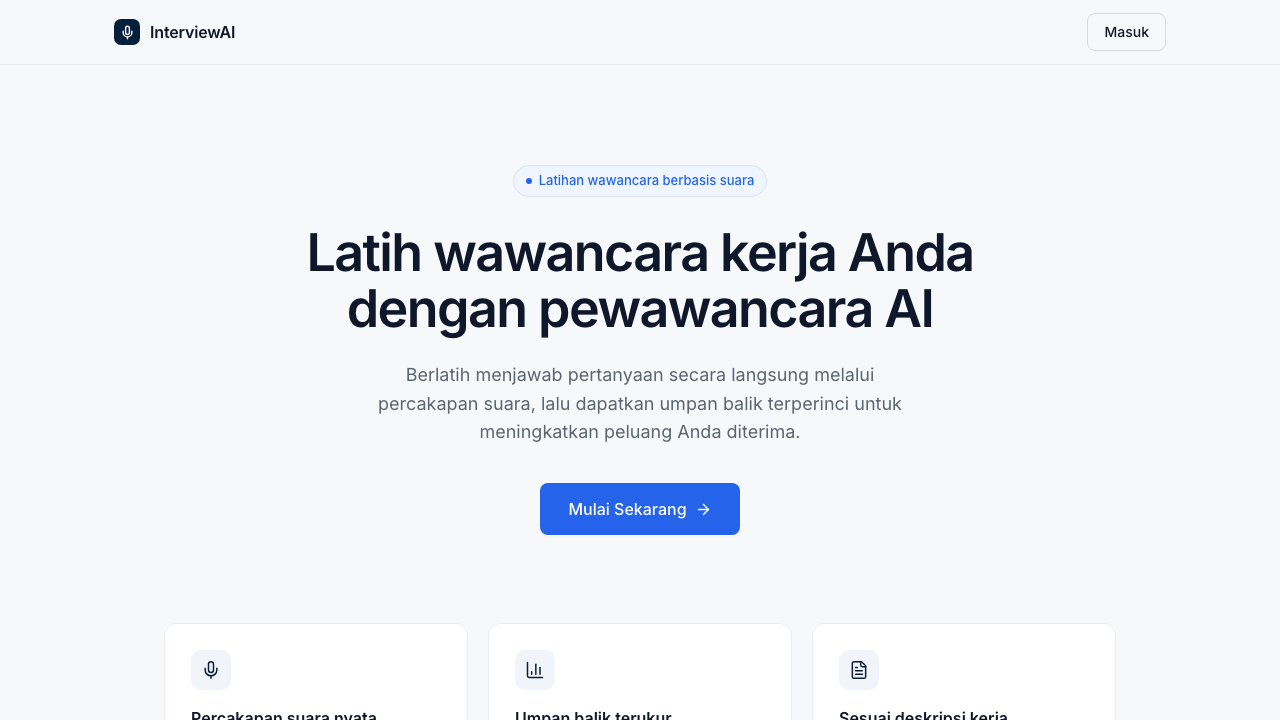
\includegraphics[width=\textwidth]{01-landing.png}
\caption{Halaman Landing}
\label{fig:landing}
\end{figure}

\begin{figure}[H]
\centering
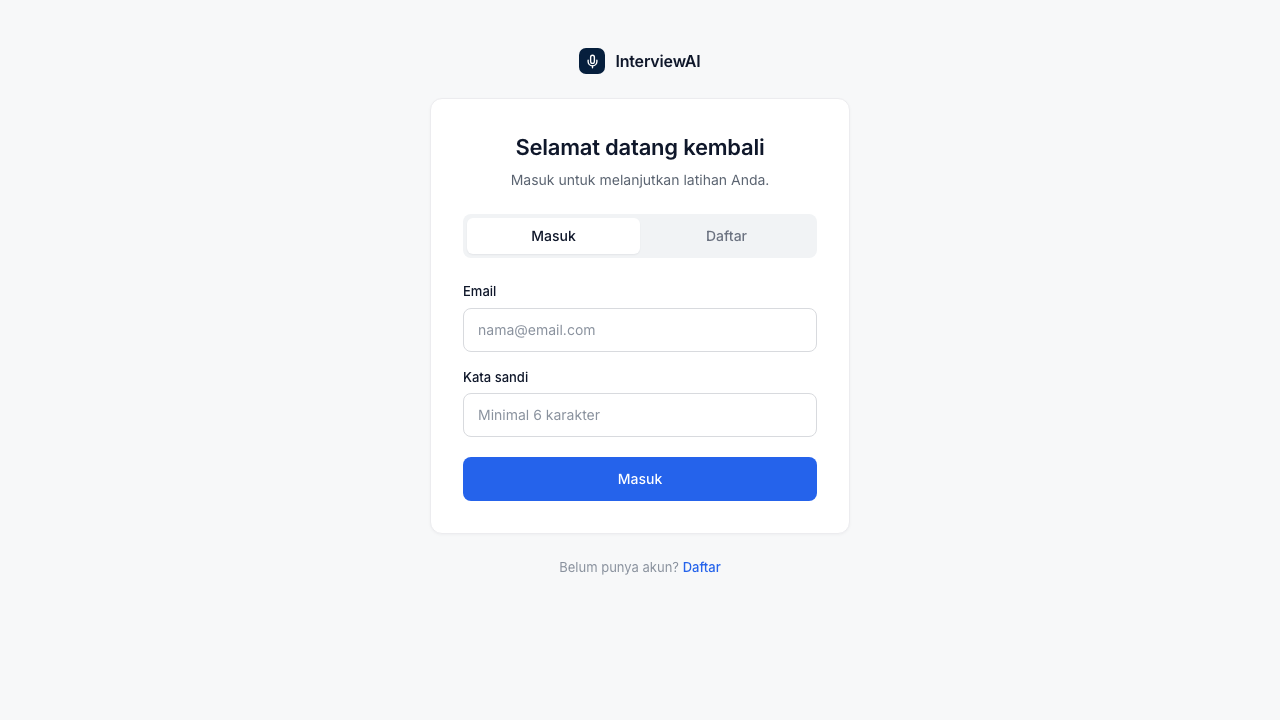
\includegraphics[width=0.8\textwidth]{02-login.png}
\caption{Halaman Login}
\label{fig:login}
\end{figure}

\begin{figure}[H]
\centering
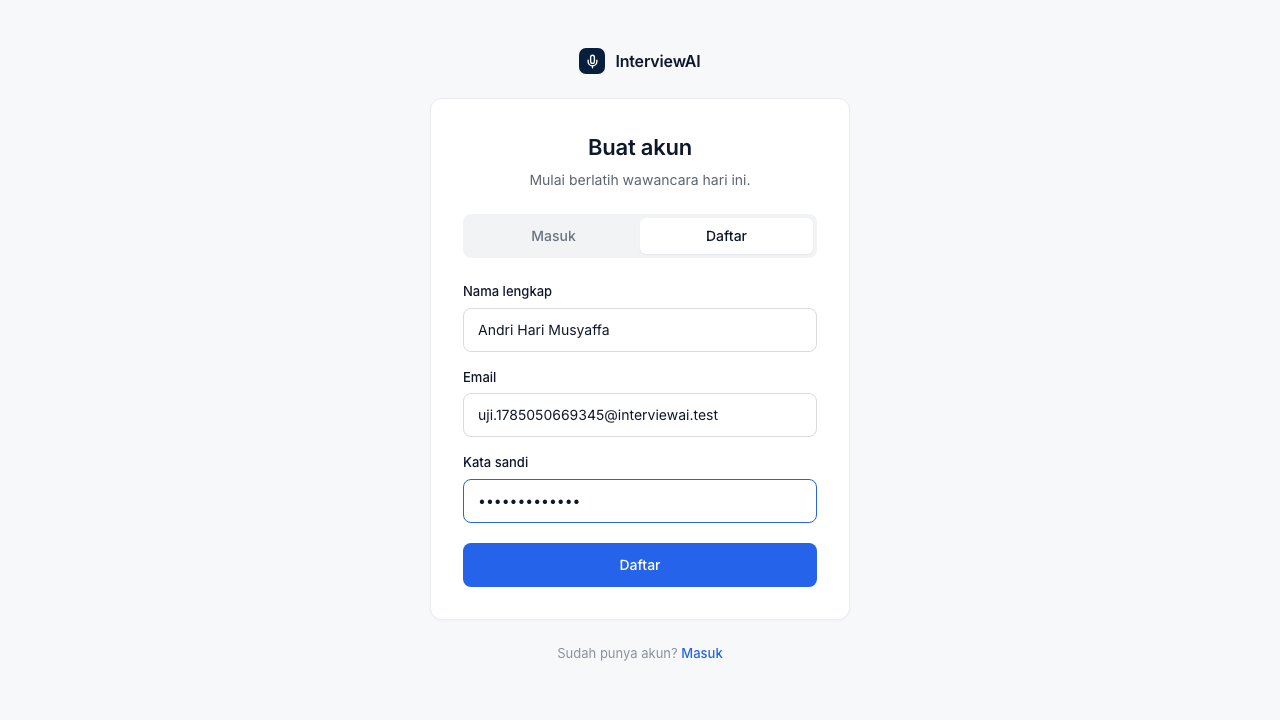
\includegraphics[width=0.8\textwidth]{03-register.png}
\caption{Halaman Register}
\label{fig:register}
\end{figure}

\begin{figure}[H]
\centering
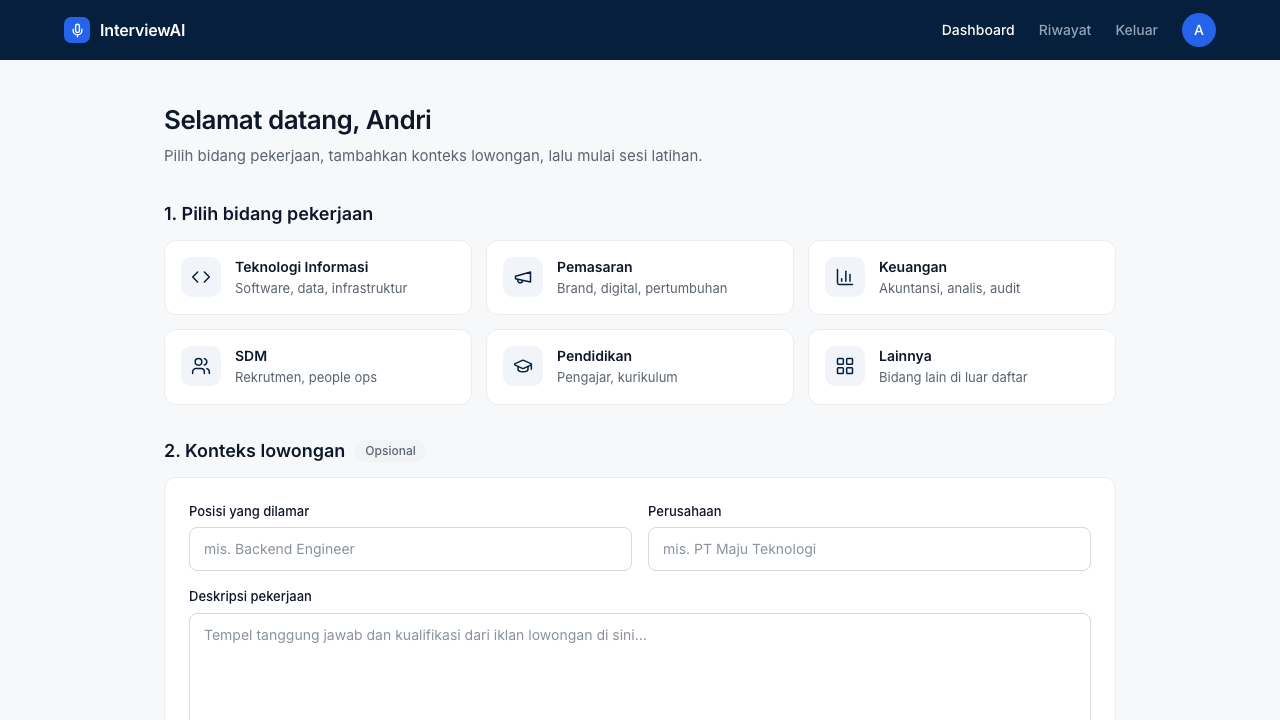
\includegraphics[width=\textwidth]{04-dashboard.png}
\caption{Halaman Dashboard --- Pemilihan Bidang Pekerjaan}
\label{fig:dashboard}
\end{figure}

\begin{figure}[H]
\centering
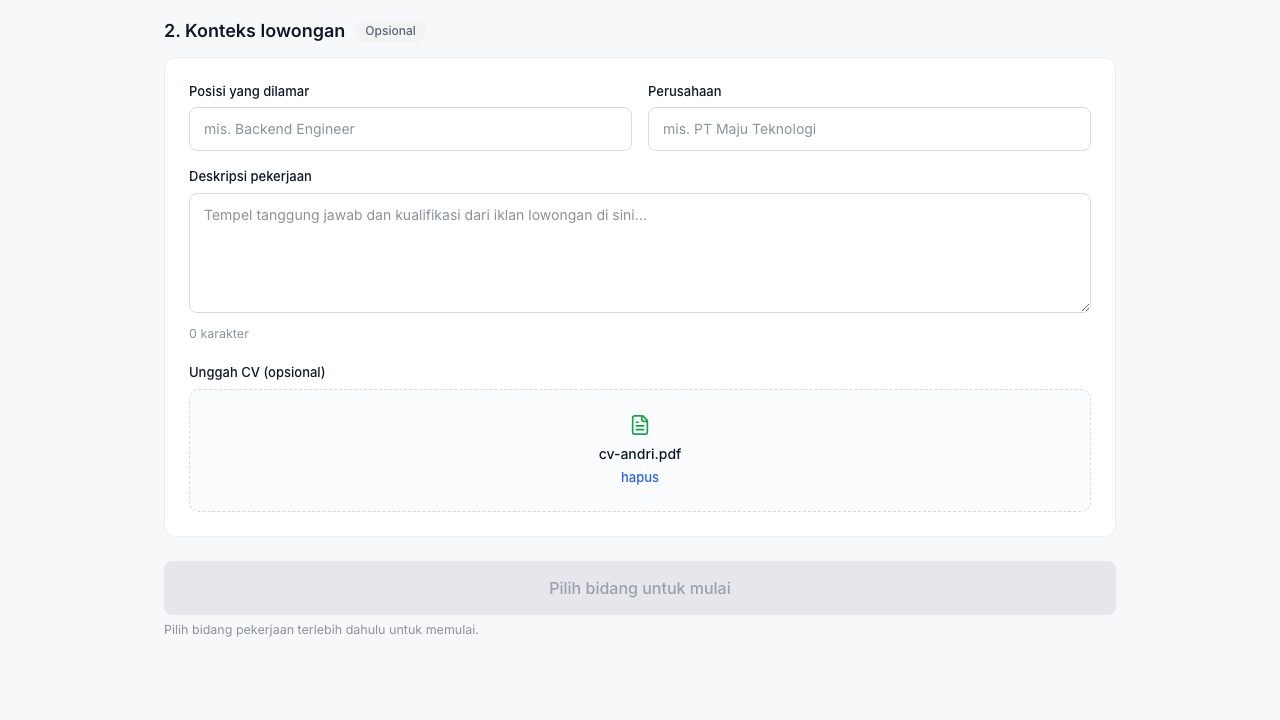
\includegraphics[width=\textwidth]{05-upload-cv.png}
\caption{Formulir Konteks Lowongan dan Unggah CV}
\label{fig:upload-cv}
\end{figure}

\begin{figure}[H]
\centering
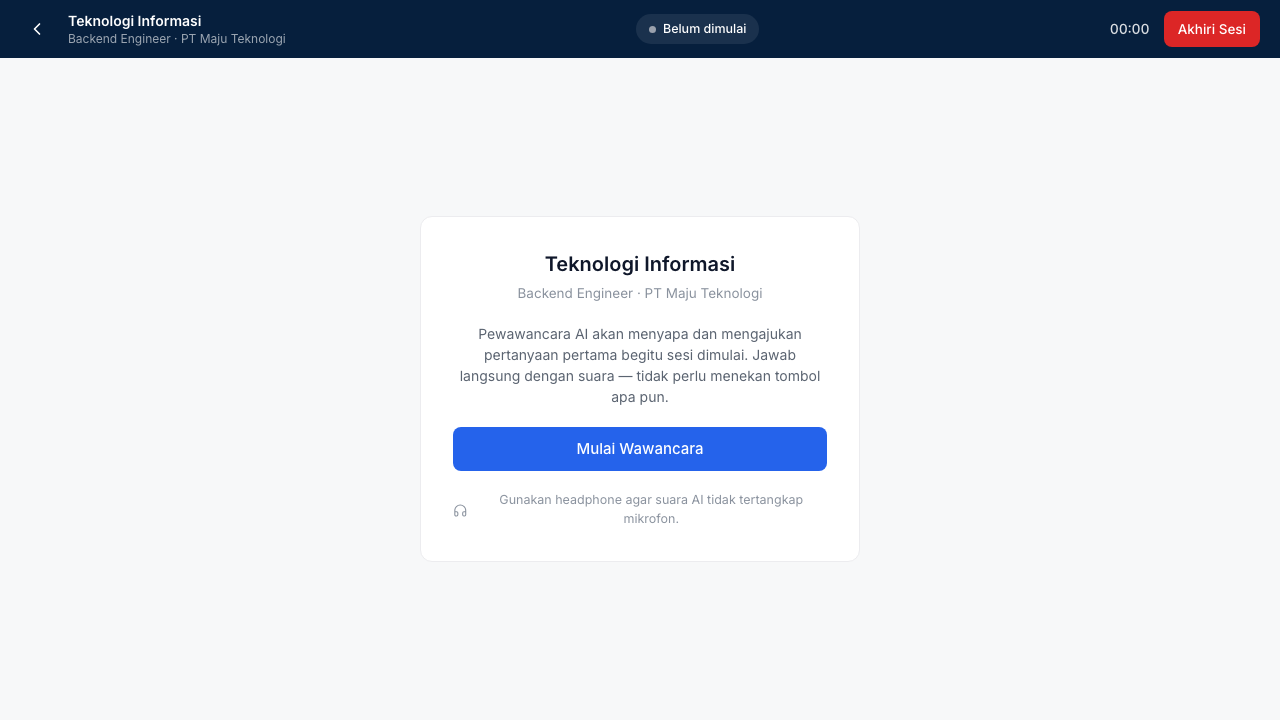
\includegraphics[width=\textwidth]{06-pre-session.png}
\caption{Halaman Persiapan Sesi Wawancara}
\label{fig:pre-session}
\end{figure}

\begin{figure}[H]
\centering
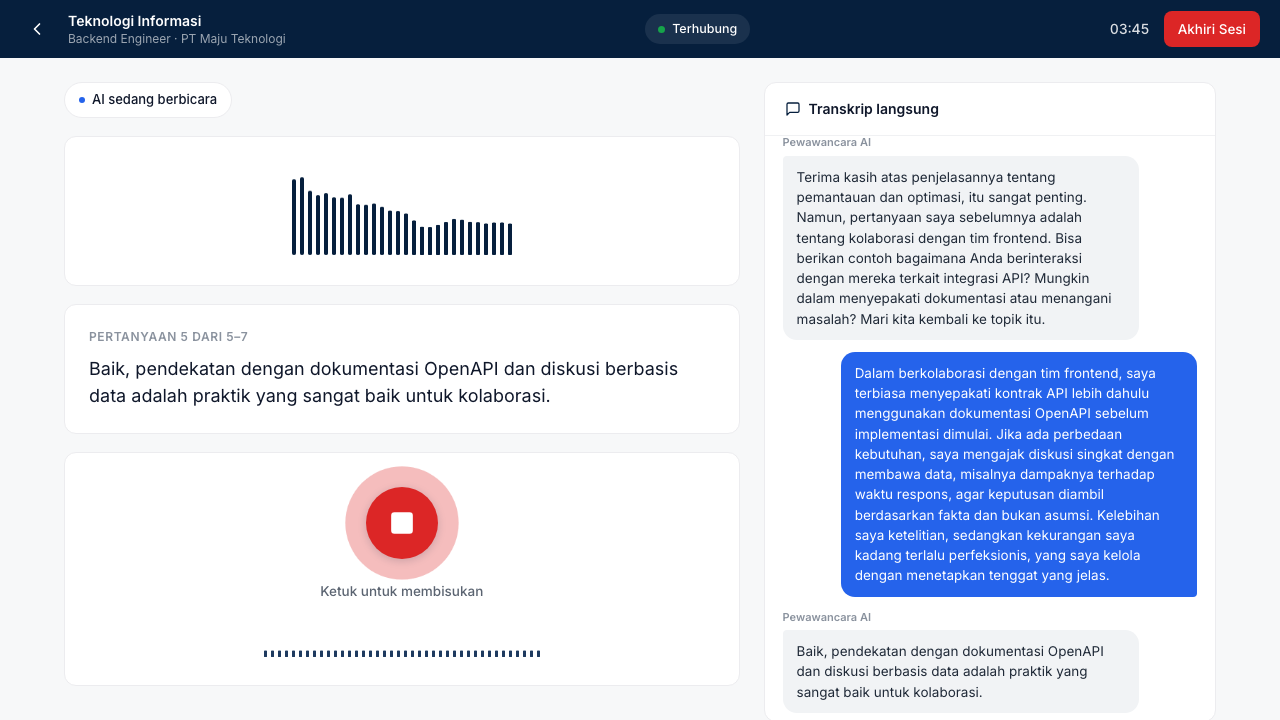
\includegraphics[width=\textwidth]{07-session-live.png}
\caption{Halaman Sesi Wawancara Berlangsung}
\label{fig:session-live}
\end{figure}

Gambar~\ref{fig:session-live} memperlihatkan sesi wawancara yang sedang
berjalan. Kolom kiri menampilkan indikator status pembicara, visualisasi
amplitudo audio, kartu pertanyaan terakhir, dan kendali mikrofon; sedangkan
kolom kanan menampilkan transkrip percakapan secara berurutan. Indikator
``Terhubung'' pada bilah atas menandakan koneksi \textit{WebSocket} ke Gemini
Live API dalam keadaan aktif, dan penghitung waktu menunjukkan durasi sesi
yang sedang berjalan.

\begin{figure}[H]
\centering
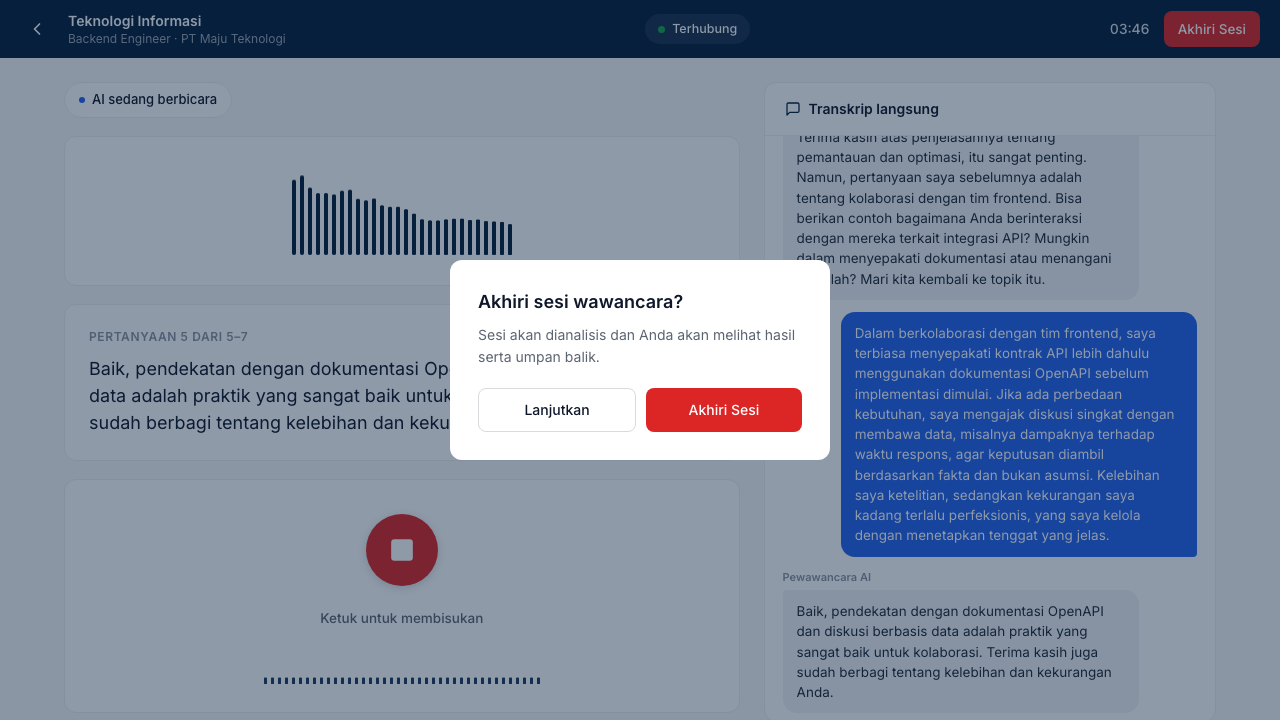
\includegraphics[width=\textwidth]{08-end-confirm.png}
\caption{Dialog Konfirmasi Pengakhiran Sesi}
\label{fig:end-confirm}
\end{figure}

\begin{figure}[H]
\centering
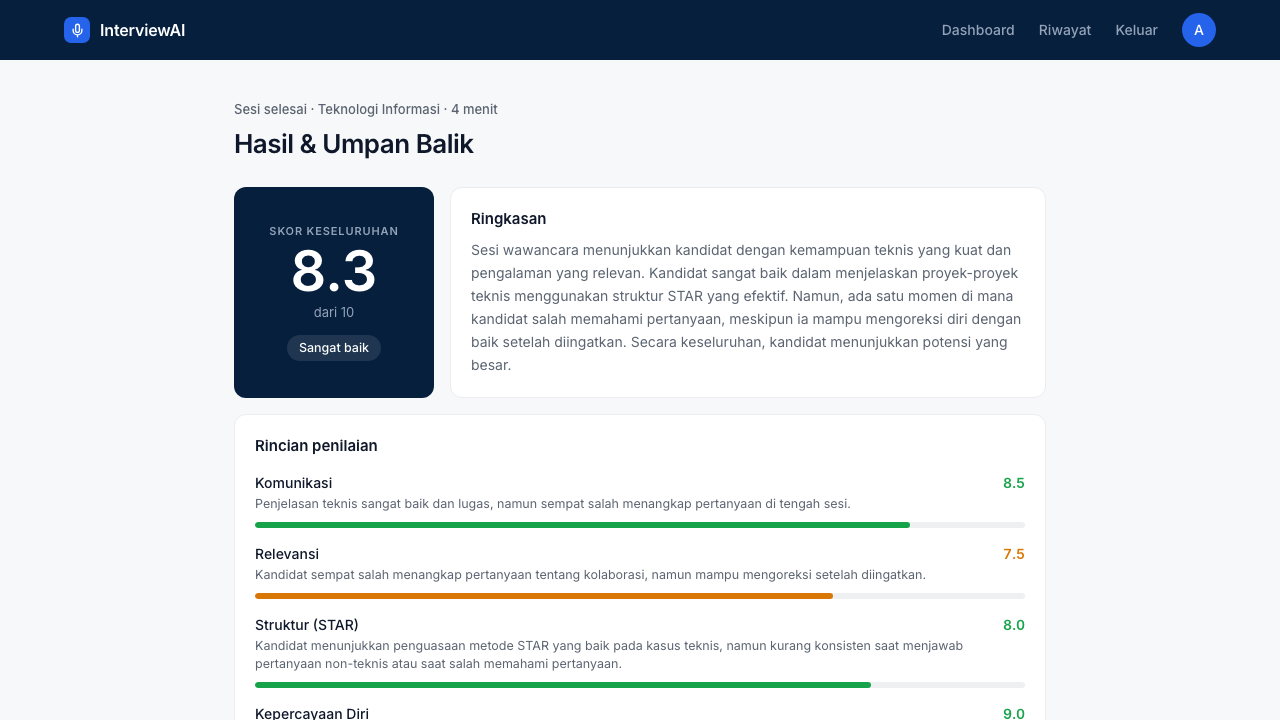
\includegraphics[width=\textwidth]{09-result.png}
\caption{Halaman Hasil dan Umpan Balik}
\label{fig:result}
\end{figure}

\begin{figure}[H]
\centering
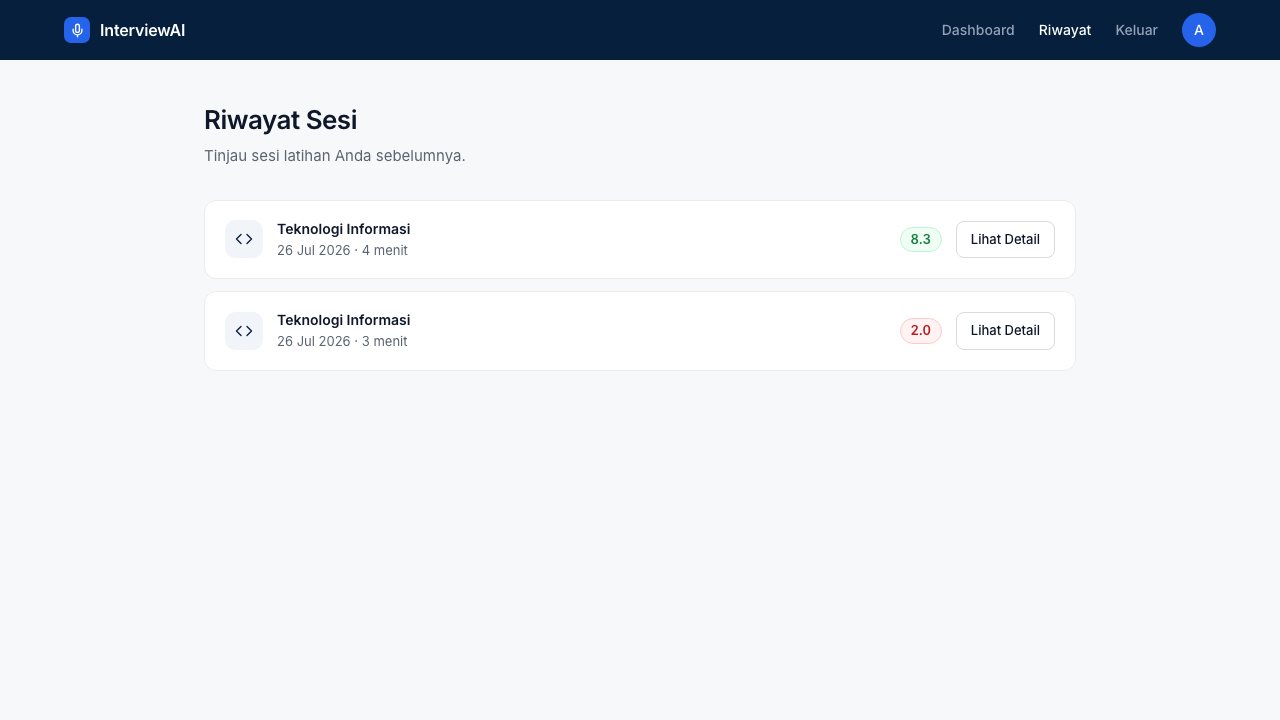
\includegraphics[width=\textwidth]{10-history.png}
\caption{Halaman Riwayat Sesi}
\label{fig:history}
\end{figure}

\begin{figure}[H]
\centering
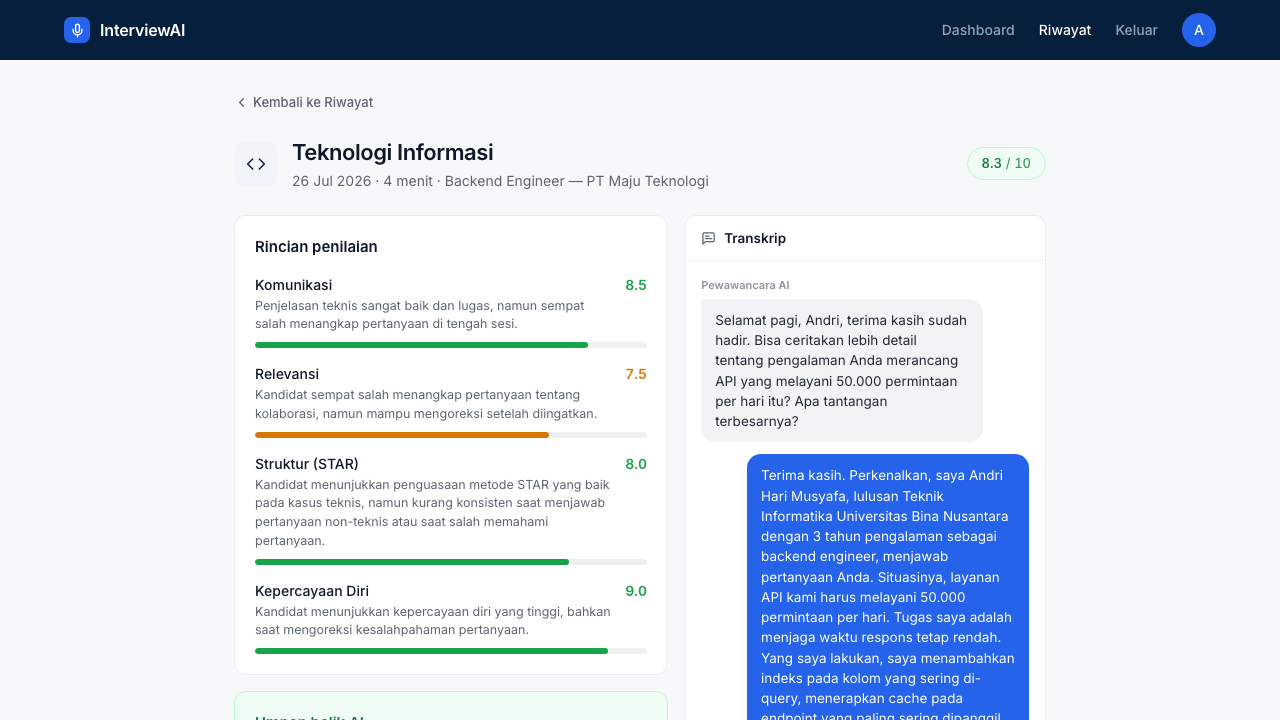
\includegraphics[width=\textwidth]{11-history-detail.png}
\caption{Halaman Detail Riwayat Sesi}
\label{fig:history-detail}
\end{figure}

\subsection{Implementasi Integrasi Gemini Live API}

Integrasi dengan Gemini Live API merupakan bagian paling kompleks dari sistem
ini karena melibatkan komunikasi audio dua arah secara \textit{real-time}.
Implementasinya menerapkan pola \textit{token broker}, yaitu \textit{backend}
tidak meneruskan aliran audio, melainkan hanya menerbitkan
\textit{ephemeral token} berumur pendek yang kemudian digunakan peramban untuk
membuka koneksi \textit{WebSocket Secure} langsung ke Gemini.

Alur satu sesi wawancara berjalan sebagai berikut:

\begin{enumerate}[leftmargin=*,itemsep=2pt]
  \item Pengguna memilih bidang pekerjaan, mengisi konteks lowongan, dan
        secara opsional mengunggah CV, lalu sistem membuat data sesi melalui
        \texttt{POST /api/sessions}.
  \item Peramban meminta \textit{ephemeral token} melalui
        \texttt{POST /api/sessions/:id/token}. Pada titik inilah
        \textit{backend} menyusun \textit{system instruction} yang berisi
        persona pewawancara beserta konteks sesi dan teks CV, lalu menguncinya
        di sisi server melalui \texttt{liveConnectConstraints}.
  \item Peramban membuka koneksi \textit{WebSocket} langsung ke Gemini
        menggunakan token tersebut, lalu mengirimkan perintah pembuka agar AI
        menyapa dan langsung mengajukan pertanyaan pertama.
  \item Audio mikrofon direkam pada 16 kHz, dikonversi menjadi PCM 16-bit di
        dalam \textit{AudioWorklet}, dan dikirimkan secara terus-menerus.
        Balasan audio Gemini pada 24 kHz diantrikan dan diputar kembali.
  \item Ketika pengguna mengakhiri sesi, transkrip dikirim ke
        \texttt{POST /api/sessions/}\linebreak[1]\texttt{:id/analyze} untuk dievaluasi, kemudian
        \texttt{POST /api/sessions/:id/end} menuliskan transkrip ke MongoDB
        lebih dahulu sebelum menandai sesi sebagai selesai di PostgreSQL.
\end{enumerate}

Parameter konfigurasi Gemini Live API hasil implementasi ditunjukkan pada
Tabel~\ref{tab:param-live}.

\begin{table}[H]
\caption{Parameter Konfigurasi Gemini Live API Hasil Implementasi}
\label{tab:param-live}
\centering
\begin{tabularx}{\textwidth}{|L{3.4cm}|L{4.2cm}|X|}
\hline
\textbf{Parameter} & \textbf{Nilai} & \textbf{Keterangan} \\
\hline
\textit{Model} & \texttt{gemini-3.1-flash-}\linebreak\texttt{live-preview} & Model \textit{native audio} dengan latensi terendah yang tersedia \\
\hline
Versi API & \texttt{v1alpha} & Versi yang menyediakan \textit{ephemeral token} \\
\hline
\textit{Response modalities} & \texttt{AUDIO} & Keluaran utama berupa audio \\
\hline
Transkripsi & \textit{input} dan \textit{output} diaktifkan & Menghasilkan transkrip dua arah untuk layar dan evaluasi \\
\hline
Format audio masuk & PCM 16-bit, 16 kHz, mono & Format yang diminta Gemini Live API \\
\hline
Format audio keluar & PCM 16-bit, 24 kHz, mono & Format balasan Gemini \\
\hline
\textit{Language code} & \texttt{id-ID} & Bahasa Indonesia \\
\hline
\textit{Voice} & \texttt{Kore} & Suara pewawancara AI \\
\hline
\textit{Temperature} & 0,7 & Keseimbangan variasi dan konsistensi respons \\
\hline
Masa berlaku token & 30 menit, sekali pakai & Membatasi dampak apabila token bocor \\
\hline
\end{tabularx}
\end{table}

\subsection{Implementasi Personalisasi Berbasis CV}

Berkas CV yang diunggah dalam format PDF maupun DOCX diekstraksi teksnya di
sisi \textit{backend}, lalu disisipkan ke dalam \textit{system instruction}
dengan batas maksimum 8.000 karakter. Pembatasan ini diperlukan karena
\textit{prompt} yang terlalu panjang meningkatkan biaya token sekaligus
latensi pada setiap sesi.

Efektivitas personalisasi ini terbukti pada saat pengujian. CV yang digunakan
memuat butir pengalaman berupa perancangan layanan API yang melayani 50.000
permintaan per hari. Pertanyaan pertama yang diajukan pewawancara AI adalah:

\begin{quote}
\textit{``Selamat pagi, Andri, terima kasih sudah hadir. Bisa ceritakan lebih
detail tentang pengalaman Anda merancang API yang melayani 50.000 permintaan
per hari itu? Apa tantangan terbesarnya?''}
\end{quote}

Pertanyaan tersebut menyebut angka yang hanya terdapat di dalam berkas CV,
sehingga membuktikan bahwa teks CV benar-benar terekstraksi, tersisipkan ke
dalam \textit{system instruction}, dan digunakan oleh model untuk menyusun
pertanyaan yang personal.

\subsection{Implementasi Evaluasi Terstruktur}

Evaluasi tidak dihasilkan oleh model percakapan, melainkan oleh model teks
terpisah (\texttt{gemini-2.5-flash}) yang menerima seluruh transkrip sesi.
Model diminta mengembalikan keluaran JSON terstruktur melalui mekanisme
\textit{response schema}, dengan empat metrik tetap yaitu Komunikasi,
Relevansi, Struktur (STAR), dan Kepercayaan Diri.

Karena keluaran model bahasa tetap berpotensi menyimpang dari skema yang
diminta, hasilnya melewati proses normalisasi sebelum disimpan. Proses ini
mencocokkan metrik berdasarkan \textit{key} maupun \textit{label},
membatasi setiap skor pada rentang 0--100, serta mengisi nilai cadangan
apabila ada bagian yang kosong. Dengan demikian bentuk data evaluasi yang
diterima antarmuka selalu konsisten, meskipun respons model bervariasi.

\subsection{Implementasi Keamanan}

Aspek keamanan yang berhasil diimplementasikan dirangkum pada
Tabel~\ref{tab:keamanan}.

\begin{table}[H]
\caption{Mekanisme Keamanan yang Diimplementasikan}
\label{tab:keamanan}
\centering
\begin{tabularx}{\textwidth}{|L{4.4cm}|X|}
\hline
\textbf{Aspek} & \textbf{Implementasi} \\
\hline
Kerahasiaan kunci API & Kunci API Gemini hanya berada di \textit{backend}; peramban hanya menerima \textit{ephemeral token} sekali pakai berumur 30 menit \\
\hline
Integritas persona AI & Model, \textit{system instruction}, suara, dan \textit{temperature} dikunci di sisi server; klien hanya boleh mengirim \textit{session resumption handle} \\
\hline
Autentikasi & JWT \textit{access token} berumur 15 menit dan \textit{refresh token} 7 hari pada \textit{cookie} \texttt{httpOnly} \\
\hline
Penyimpanan kata sandi & \textit{Hashing} menggunakan algoritma Argon2 \\
\hline
Pembatasan laju & 20 permintaan per IP tiap 15 menit pada \textit{endpoint} autentikasi, dan 40 permintaan per pengguna tiap 15 menit pada \textit{endpoint} yang memanggil Gemini \\
\hline
Otorisasi data & Setiap akses sesi maupun CV memverifikasi kepemilikan \texttt{user\_id}, dan parameter UUID divalidasi sebelum menyentuh basis data \\
\hline
Pengerasan HTTP & \textit{Helmet}, CORS dengan satu \textit{origin} dari variabel lingkungan, serta validasi variabel lingkungan saat proses \textit{boot} \\
\hline
\end{tabularx}
\end{table}

Pembatasan peran juga diterapkan pada tingkat \textit{prompt}. \textit{System
instruction} secara eksplisit melarang AI menjawab pertanyaan di luar konteks
wawancara serta mengabaikan permintaan untuk berganti peran atau membocorkan
isi instruksi, sebagai mitigasi terhadap upaya \textit{prompt injection}.

% =====================================================================
\section{Penyesuaian terhadap Rancangan BAB III}
% =====================================================================

Selama tahap implementasi ditemukan sejumlah kendala teknis yang menyebabkan
beberapa keputusan rancangan pada BAB III perlu disesuaikan. Ringkasan
penyesuaian tersebut ditunjukkan pada Tabel~\ref{tab:deviasi}, sedangkan
penyesuaian yang paling berdampak diuraikan pada sub-bab berikutnya.

\begin{table}[H]
\caption{Ringkasan Penyesuaian Rancangan terhadap Implementasi}
\label{tab:deviasi}
\centering
\begin{tabularx}{\textwidth}{|L{3.5cm}|L{3.4cm}|X|}
\hline
\textbf{Rancangan (BAB III)} & \textbf{Implementasi} & \textbf{Alasan Penyesuaian} \\
\hline
Supabase sebagai penyedia PostgreSQL, Auth, dan Storage & PostgreSQL mandiri, autentikasi JWT + Argon2 sendiri, CV disimpan pada \textit{filesystem} server & Menghilangkan ketergantungan pada layanan pihak ketiga dan biaya berlangganan, sekaligus memberi kendali penuh atas skema basis data dan masa berlaku token \\
\hline
\textit{Backend} berperan sebagai \textit{WebSocket proxy} & Pola \textit{token broker}; audio mengalir langsung dari peramban ke Gemini & \textit{Proxy} menambah satu lompatan jaringan pada jalur yang paling sensitif terhadap latensi dan membebani server dengan seluruh aliran audio. Pola \textit{token broker} tetap menjaga kerahasiaan kunci API tanpa biaya latensi tersebut \\
\hline
Model \texttt{gemini-live-}\linebreak\texttt{3-flash}, suara bawaan & \texttt{gemini-3.1-}\linebreak\texttt{flash-live-}\linebreak\texttt{preview}, suara \texttt{Kore}, \texttt{id-ID} & Nama model pada rancangan tidak tersedia. Model yang dipilih memberi waktu respons sekitar 1,5 detik dibanding sekitar 5,0 detik pada alternatifnya \\
\hline
Evaluasi berupa \texttt{overall\_score} dan \texttt{feedback\_text} & Ditambah empat metrik terstruktur, \texttt{strengths}, \texttt{improvements}, dan \texttt{summary} & Skor tunggal tidak cukup informatif sebagai bahan perbaikan. Penilaian per aspek menjawab kebutuhan umpan balik yang dapat ditindaklanjuti \\
\hline
Tipe kunci utama pada \texttt{job\_fields} adalah SERIAL & Bertipe UUID & Menyeragamkan tipe kunci seluruh tabel sehingga tidak ada identitas yang mudah ditebak berurutan \\
\hline
\textit{Deployment} pada Vercel dan Cloud Run & Direncanakan pada VPS di belakang \textit{nginx} & Menyederhanakan operasional menjadi satu lingkungan dan menekan biaya. Tahap ini belum dilaksanakan pada penelitian ini \\
\hline
\end{tabularx}
\end{table}

\subsection{Penggantian Supabase dengan Layanan Mandiri}

Rancangan awal menempatkan Supabase sebagai penyedia PostgreSQL, autentikasi,
dan penyimpanan berkas sekaligus. Pada implementasi, ketiga peran tersebut
dipisahkan dan dikelola sendiri. PostgreSQL dijalankan secara mandiri dengan
skema yang dikelola melalui berkas migrasi SQL berurutan, autentikasi
diimplementasikan menggunakan JWT dengan \textit{hashing} Argon2, dan berkas
CV disimpan pada \textit{filesystem} server dengan nama berkas yang diacak.

Konsekuensinya, pengelolaan keamanan autentikasi menjadi tanggung jawab
sistem ini sendiri. Hal tersebut dikompensasi dengan penerapan \textit{refresh
token} pada \textit{cookie} \texttt{httpOnly}, masa berlaku \textit{access
token} yang pendek, serta pembatasan laju pada \textit{endpoint}
autentikasi.

\subsection{Perubahan Pola Integrasi menjadi \textit{Token Broker}}

Perubahan paling mendasar terjadi pada pola integrasi dengan Gemini Live API.
Rancangan BAB III menempatkan \textit{backend} sebagai \textit{WebSocket
proxy} yang meneruskan audio dari klien ke Gemini. Pendekatan tersebut
memiliki dua kelemahan: seluruh aliran audio dua arah harus melewati server
sehingga menambah beban dan biaya bandwidth, dan setiap lompatan tambahan
menambah latensi pada jalur yang justru paling menentukan kealamian
percakapan.

Pada implementasi, \textit{backend} hanya berperan menerbitkan
\textit{ephemeral token}, sedangkan koneksi \textit{WebSocket} dibuka langsung
dari peramban ke Gemini. Kerahasiaan kunci API tetap terjaga karena kunci
tersebut tidak pernah meninggalkan server, dan konfigurasi sesi dikunci pada
saat token diterbitkan sehingga klien tidak dapat mengubah persona
pewawancara, model, maupun suara yang digunakan.

\subsection{Perluasan Skema Evaluasi}

Rancangan awal hanya menyimpan skor keseluruhan dan umpan balik naratif.
Skema tersebut diperluas menjadi empat metrik penilaian beserta catatannya,
ditambah daftar kelebihan, daftar hal yang perlu ditingkatkan, dan ringkasan
sesi. Perluasan ini menjawab tujuan penelitian mengenai umpan balik yang
bersifat personal, karena pengguna dapat mengetahui aspek mana yang lemah dan
bukan sekadar menerima satu angka.

% =====================================================================
\section{Pengujian Sistem}
% =====================================================================

\subsection{Metode dan Lingkungan Pengujian}

Pengujian dilakukan menggunakan metode \textit{Black Box Testing} sesuai
rencana pada BAB III, yaitu memvalidasi fungsionalitas berdasarkan masukan dan
keluaran yang diharapkan tanpa memeriksa struktur internal kode program.
Seluruh skenario diotomasi menggunakan Playwright dan dijalankan pada peramban
Chromium, sehingga pengujian dapat diulang dan hasilnya dapat diverifikasi
kembali.

Skenario dijalankan secara berurutan dalam satu \textit{worker} karena antar
skenario terdapat ketergantungan data: sesi wawancara yang diselesaikan pada
berkas skenario ketiga merupakan data yang diperiksa oleh skenario pengujian
riwayat. Dengan demikian alur simpan dan baca lintas kedua basis data ikut
terverifikasi.

Pengujian sesi wawancara suara memerlukan sumber suara kandidat. Suara
tersebut disintesis menggunakan \textit{text-to-speech} berbahasa Indonesia
berisi lima jawaban yang disusun mengikuti kerangka STAR, dengan jeda hening
di antara jawaban agar giliran bicara tidak bertabrakan dengan suara
pewawancara AI.

Pada tahap penyiapan ditemukan bahwa opsi Chromium
\texttt{-{}-use-file-for-}\allowbreak\texttt{fake-audio-capture} tidak berpengaruh pada
lingkungan pengujian yang digunakan. Hal ini diverifikasi menggunakan berkas
uji berpola nada keras dan hening bergantian setiap satu detik: pola tersebut
sama sekali tidak muncul pada data PCM yang benar-benar dikirimkan aplikasi ke
Gemini. Oleh karena itu mikrofon disimulasikan satu lapis lebih tinggi, yaitu
dengan mengembalikan \textit{MediaStream} yang dibangkitkan Web Audio API dari
berkas suara yang sama. Yang disimulasikan hanya perangkat keras mikrofonnya,
sedangkan seluruh jalur kode aplikasi --- \textit{AudioWorklet}, konversi PCM
16 kHz, hingga pengiriman ke Gemini --- tetap berjalan apa adanya, sehingga
pengujian tetap sah sebagai pengujian \textit{Black Box} terhadap sistem.

\subsection{Skenario dan Hasil Pengujian}

Sebanyak 26 skenario pengujian disusun untuk mencakup kesebelas
\textit{use case} yang dirancang pada BAB III, mencakup kasus normal maupun
kasus negatif. Hasil pengujian selengkapnya ditunjukkan pada
Tabel~\ref{tab:hasil-uji}.

\begin{longtable}{|C{1.1cm}|C{1.1cm}|L{4.5cm}|L{3.1cm}|C{1.3cm}|}
\caption{Hasil Pengujian \textit{Black Box}}
\label{tab:hasil-uji} \\
\hline
\textbf{Kode} & \textbf{UC} & \textbf{Skenario Pengujian} & \textbf{Hasil yang Diharapkan} & \textbf{Hasil} \\
\hline
\endfirsthead
\multicolumn{5}{l}{\small\textit{Lanjutan Tabel \ref{tab:hasil-uji}}} \\
\hline
\textbf{Kode} & \textbf{UC} & \textbf{Skenario Pengujian} & \textbf{Hasil yang Diharapkan} & \textbf{Hasil} \\
\hline
\endhead
\hline
\endfoot
\hline
\endlastfoot

TC-00 & -- & Membuka halaman Landing & Judul dan tombol ``Mulai Sekarang'' tampil & Valid \\
\hline
TC-01 & UC-02 & Membuka Dashboard tanpa autentikasi & Dialihkan ke halaman Login & Valid \\
\hline
TC-02 & UC-01 & Register dengan format email tidak valid & Pesan ``Masukkan email yang valid'' tampil & Valid \\
\hline
TC-03 & UC-01 & Register dengan kata sandi kurang dari 6 karakter & Pesan ``Kata sandi minimal 6 karakter'' tampil & Valid \\
\hline
TC-04 & UC-01 & Register dengan data lengkap dan valid & Akun terbentuk dan masuk ke Dashboard & Valid \\
\hline
TC-05 & UC-01 & Register dengan email yang sudah terdaftar & Ditolak server dengan pesan galat & Valid \\
\hline
TC-06 & UC-02 & Login dengan kata sandi salah & Ditolak dan tetap di halaman Login & Valid \\
\hline
TC-07 & UC-02 & Login dengan kredensial benar & Masuk ke Dashboard & Valid \\
\hline
TC-08 & UC-10 & Menekan tombol Keluar & Sesi berakhir dan halaman terproteksi diblokir & Valid \\
\hline
TC-09 & UC-03 & Memuat daftar bidang pekerjaan & Enam bidang pekerjaan tampil dari server & Valid \\
\hline
TC-10 & UC-03 & Belum memilih bidang pekerjaan & Tombol mulai sesi dalam keadaan nonaktif & Valid \\
\hline
TC-11 & UC-03 & Memilih salah satu bidang pekerjaan & Tombol mulai sesi menjadi aktif & Valid \\
\hline
TC-12 & UC-03 & Mengisi deskripsi lowongan lebih dari 40 karakter & Konfirmasi ``Konteks akan dipakai AI'' tampil & Valid \\
\hline
TC-13 & UC-11 & Mengunggah CV berformat PDF & Berkas terunggah dan teksnya terekstraksi & Valid \\
\hline
TC-14 & UC-11 & Mengunggah CV berformat DOCX & Berkas terunggah dan teksnya terekstraksi & Valid \\
\hline
TC-15 & UC-11 & Mengunggah berkas berformat selain PDF/DOCX & Ditolak dengan pesan format tidak sesuai & Valid \\
\hline
TC-16 & UC-11 & Menghapus CV yang telah diunggah & Formulir kembali ke keadaan semula & Valid \\
\hline
TC-17 & UC-04 & Menekan tombol Mulai Sesi Wawancara & Sesi terbentuk dan halaman wawancara terbuka & Valid \\
\hline
TC-18 & UC-04 & Memulai wawancara & Koneksi terbuka dan AI menyapa serta bertanya & Valid \\
\hline
TC-19 & UC-05 & Kandidat menjawab dengan suara & Jawaban tertranskripsi pada panel transkrip & Valid \\
\hline
TC-20 & UC-06 & Melanjutkan percakapan beberapa giliran & AI menanggapi jawaban dan mengajukan pertanyaan lanjutan & Valid \\
\hline
TC-21 & UC-07 & Mengakhiri sesi wawancara & Evaluasi dihasilkan dan halaman Hasil tampil lengkap & Valid \\
\hline
TC-22 & UC-08 & Membuka halaman Riwayat & Sesi yang telah selesai tampil beserta skornya & Valid \\
\hline
TC-23 & UC-09 & Membuka detail salah satu sesi & Rincian penilaian dan transkrip tampil & Valid \\
\hline
TC-24 & UC-09 & Membuka detail sesi milik pengguna lain & Akses ditolak dan pesan galat tampil & Valid \\
\hline
TC-25 & UC-09 & Kembali dari detail ke daftar riwayat & Kembali ke halaman Riwayat & Valid \\
\hline
\end{longtable}

\subsection{Analisis Persentase Keberhasilan}

Persentase keberhasilan dihitung menggunakan rumus yang telah ditetapkan pada
BAB III, yaitu:

\begin{center}
\textit{Success Rate} $=\dfrac{\text{Jumlah \textit{test case} valid}}{\text{Total \textit{test case}}}\times 100\%$
\end{center}

Rekapitulasi hasil pengujian per \textit{use case} ditunjukkan pada
Tabel~\ref{tab:success-rate}.

\begin{table}[H]
\caption{Rekapitulasi Persentase Keberhasilan per \textit{Use Case}}
\label{tab:success-rate}
\centering
\begin{tabularx}{\textwidth}{|C{1.6cm}|X|C{1.9cm}|C{1.6cm}|C{2.1cm}|}
\hline
\textbf{Kode UC} & \textbf{Nama \textit{Use Case}} & \textbf{Jumlah \textit{Test Case}} & \textbf{Valid} & \textbf{Persentase} \\
\hline
UC-01 & Register & 4 & 4 & 100\% \\
\hline
UC-02 & Login & 3 & 3 & 100\% \\
\hline
UC-03 & Memilih Bidang Pekerjaan & 4 & 4 & 100\% \\
\hline
UC-04 & Memulai Sesi Wawancara & 2 & 2 & 100\% \\
\hline
UC-05 & Menjawab Pertanyaan & 1 & 1 & 100\% \\
\hline
UC-06 & Menerima Umpan Balik & 1 & 1 & 100\% \\
\hline
UC-07 & Mengakhiri Sesi & 1 & 1 & 100\% \\
\hline
UC-08 & Melihat Riwayat Sesi & 1 & 1 & 100\% \\
\hline
UC-09 & Melihat Detail Riwayat & 3 & 3 & 100\% \\
\hline
UC-10 & Logout & 1 & 1 & 100\% \\
\hline
UC-11 & Mengunggah CV & 4 & 4 & 100\% \\
\hline
-- & Umum (halaman Landing) & 1 & 1 & 100\% \\
\hline
\multicolumn{2}{|c|}{\textbf{Total}} & \textbf{26} & \textbf{26} & \textbf{100\%} \\
\hline
\end{tabularx}
\end{table}

Berdasarkan rekapitulasi tersebut, seluruh 26 \textit{test case} dinyatakan
valid sehingga persentase keberhasilan mencapai 100\%. Nilai ini melampaui
ambang minimal 90\% untuk setiap kategori fitur yang ditetapkan pada BAB III,
sehingga hipotesis penelitian mengenai keberhasilan fungsional sistem
dinyatakan terpenuhi.

% =====================================================================
\section{Pembahasan}
% =====================================================================

\subsection{Ketercapaian Tujuan Penelitian}

Rumusan masalah pertama mempertanyakan bagaimana merancang dan membangun
\textit{website} simulasi wawancara kerja berbasis \textit{Large Language
Model} dengan memanfaatkan Gemini Live API. Hasil implementasi menunjukkan
bahwa sistem tersebut berhasil dibangun secara utuh, mulai dari autentikasi,
konfigurasi sesi, wawancara suara \textit{real-time}, evaluasi otomatis,
hingga riwayat sesi. Sistem berjalan sepenuhnya di dalam peramban tanpa
memerlukan pemasangan perangkat lunak tambahan, dan seluruh antarmukanya
menggunakan Bahasa Indonesia sehingga dapat diakses oleh pencari kerja di
Indonesia tanpa hambatan bahasa maupun biaya sesi.

Rumusan masalah kedua mempertanyakan bagaimana mengintegrasikan fitur
pertanyaan otomatis, penilaian jawaban, umpan balik personal, dan komunikasi
suara \textit{real-time} ke dalam satu \textit{platform} berbasis web.
Keempat fitur tersebut terbukti berjalan dalam satu alur yang berkesinambungan
sebagaimana ditunjukkan pada pengujian TC-17 sampai TC-21. Pertanyaan
dihasilkan secara otomatis dan dipersonalisasi berdasarkan CV, jawaban
disampaikan melalui suara dan tertranskripsi, umpan balik lisan diberikan di
sela percakapan, serta penilaian tertulis per aspek disajikan setelah sesi
berakhir.

\subsection{Analisis Kinerja Percakapan \textit{Real-time}}

Pengukuran kinerja diambil langsung pada saat pengujian sesi wawancara
berlangsung dan dirangkum pada Tabel~\ref{tab:kinerja}.

\begin{table}[H]
\caption{Hasil Pengukuran Kinerja Sesi Wawancara}
\label{tab:kinerja}
\centering
\begin{tabularx}{\textwidth}{|X|C{3cm}|}
\hline
\textbf{Aspek yang Diukur} & \textbf{Hasil} \\
\hline
Waktu dari penekanan tombol mulai hingga AI mengucapkan sapaan pertama & 2,2 detik \\
\hline
Waktu dari mulai berbicara hingga jawaban muncul pada panel transkrip & 58,1 detik\footnotemark \\
\hline
Jumlah giliran bicara pewawancara AI dalam satu sesi & 5 giliran \\
\hline
Jumlah giliran bicara kandidat dalam satu sesi & 4 giliran \\
\hline
Total panjang transkrip jawaban kandidat & 1.856 karakter \\
\hline
Waktu pembuatan evaluasi setelah sesi diakhiri & 11,9 detik \\
\hline
\end{tabularx}
\end{table}
\footnotetext{Angka ini mencakup jeda hening 17 detik pada awal berkas suara
uji dan durasi pengucapan jawaban itu sendiri, sehingga bukan merupakan
latensi transkripsi murni. Latensi transkripsi terukur berada pada kisaran 3
detik di belakang penutur.}

Waktu tanggap awal sebesar 2,2 detik menunjukkan bahwa pola \textit{token
broker} tidak menimbulkan penundaan yang terasa, meskipun peramban harus
meminta token ke \textit{backend} terlebih dahulu sebelum membuka koneksi ke
Gemini. Adapun waktu pembuatan evaluasi sebesar 11,9 detik masih dapat
diterima karena berlangsung sekali di akhir sesi dan disertai indikator
pemuatan pada antarmuka.

Karakteristik penting yang ditemukan pada tahap implementasi adalah bahwa
transkripsi masukan dari Gemini berjalan sekitar tiga detik di belakang
penutur. Akibatnya, indikator ``sedang berbicara'' pada antarmuka tidak dapat
mengandalkan transkrip tersebut. Sistem mengatasinya dengan mendeteksi
amplitudo suara secara lokal di peramban, dan sinyal tersebut digunakan
semata-mata untuk keperluan tampilan, tidak pernah untuk menggerbang
pengiriman audio ke Gemini.

\subsection{Analisis Kualitas Evaluasi}

Selama tahap pengujian dilakukan dua kali sesi wawancara dengan naskah jawaban
yang berbeda, dan perbandingan hasilnya ditunjukkan pada
Tabel~\ref{tab:banding-evaluasi}.

\begin{table}[H]
\caption{Perbandingan Hasil Evaluasi terhadap Dua Naskah Jawaban}
\label{tab:banding-evaluasi}
\centering
\begin{tabularx}{\textwidth}{|X|C{2.4cm}|C{2.4cm}|}
\hline
\textbf{Karakteristik Naskah Jawaban} & \textbf{Skor Keseluruhan} & \textbf{Skor Relevansi} \\
\hline
Jawaban umum yang tidak menanggapi pertanyaan spesifik pewawancara & 2,0 & 1,5 \\
\hline
Jawaban terstruktur STAR yang menanggapi pokok pertanyaan & 8,3 & tinggi \\
\hline
\end{tabularx}
\end{table}

Perbedaan skor yang lebar antara kedua naskah menunjukkan bahwa mekanisme
evaluasi bersifat diskriminatif, yaitu benar-benar menilai isi dan relevansi
jawaban dan bukan sekadar memberikan skor tinggi secara seragam. Pada naskah
pertama, sistem secara tepat mengidentifikasi bahwa kandidat berulang kali
tidak menjawab pertanyaan yang diajukan, dan hal tersebut tercermin pada skor
Relevansi yang rendah. Temuan ini memperkuat keyakinan bahwa umpan balik yang
dihasilkan sistem memiliki nilai diagnostik bagi pengguna.

\subsection{Keterbatasan Sistem}

Berdasarkan hasil implementasi dan pengujian, terdapat sejumlah keterbatasan
yang perlu dicatat:

\begin{enumerate}[leftmargin=*,itemsep=3pt]
  \item \textbf{Ketergantungan pada model \textit{preview}.} Model
        \texttt{gemini-3.1-flash-}\allowbreak\texttt{live-preview} berstatus
        \textit{preview}
        sehingga berpotensi berubah atau dihentikan sewaktu-waktu. Sistem
        belum memiliki mekanisme peralihan otomatis ke model cadangan.
  \item \textbf{Penentuan batas giliran bicara bersifat heuristik.} Karena
        Gemini tidak menyertakan penanda waktu pengucapan pada setiap potongan
        transkrip, sistem menentukan giliran berdasarkan waktu kedatangan
        data. Pada kondisi tertentu, beberapa kata terakhir sebuah jawaban
        dapat tergeser ke giliran berikutnya, meskipun isi dan urutan
        percakapan secara keseluruhan tetap terjaga.
  \item \textbf{Penilaian terbatas pada aspek verbal.} Sesuai ruang lingkup
        pada BAB III, sistem tidak menilai aspek psikologis maupun bahasa
        tubuh, karena masukannya hanya berupa suara.
  \item \textbf{Pengujian belum mencakup keberagaman pengguna nyata.}
        Pengujian dilakukan menggunakan suara sintetis pada satu lingkungan
        peramban. Variasi aksen, kecepatan bicara, kualitas mikrofon, dan
        kondisi kebisingan pengguna nyata belum terwakili.
  \item \textbf{Tahap \textit{deployment} belum dilaksanakan.} Sistem baru
        berjalan pada lingkungan pengembangan lokal, sehingga pengujian
        performa pada kondisi produksi belum dapat dilakukan.
\end{enumerate}

\end{document}
. Bila
% disisipkan, preamble di bawah diabaikan secara otomatis.
% =====================================================================
\documentclass[12pt,a4paper,oneside]{report}

\usepackage[T1]{fontenc}
\usepackage[utf8]{inputenc}
\usepackage{newtxtext,newtxmath}          % Times New Roman
\usepackage[bahasa]{babel}
\usepackage[a4paper,left=4cm,right=3cm,top=3cm,bottom=3cm]{geometry}
\usepackage{setspace}
\usepackage{graphicx}
\usepackage{array}
\usepackage{longtable}
\usepackage{tabularx}
\usepackage{ragged2e}
\usepackage{enumitem}
\usepackage{caption}
\usepackage{float}
\usepackage{titlesec}
\usepackage[hidelinks]{hyperref}

% Judul bab bergaya skripsi: "BAB IV" di atas, judul bab di bawahnya, keduanya
% rata tengah dan huruf kapital.
\titleformat{\chapter}[display]
  {\normalfont\bfseries\centering}
  {\Large BAB \Roman{chapter}}{12pt}{\Large}
\titlespacing*{\chapter}{0pt}{0pt}{28pt}

\graphicspath{{gambar/}}

% Judul tabel di atas, judul gambar di bawah, keduanya rata tengah dan tebal.
\captionsetup[table]{position=top,labelsep=space,font=bf,justification=centering}
\captionsetup[figure]{position=bottom,labelsep=space,font=bf,justification=centering}

\newcolumntype{L}[1]{>{\RaggedRight\arraybackslash}p{#1}}
\newcolumntype{C}[1]{>{\Centering\arraybackslash}p{#1}}

\setlength{\emergencystretch}{3em}

\setcounter{chapter}{3}   % bab berikutnya menjadi BAB IV
\onehalfspacing

\begin{document}

\chapter{HASIL DAN PEMBAHASAN}

Bab ini menyajikan hasil tahap implementasi dan tahap pengujian dari metode
pengembangan \textit{Waterfall} yang telah diuraikan pada BAB III. Pembahasan
dimulai dari lingkungan implementasi dan wujud sistem yang berhasil dibangun,
dilanjutkan dengan penjelasan mengenai penyesuaian yang dilakukan terhadap
rancangan awal beserta alasan teknisnya, kemudian hasil pengujian
\textit{Black Box} atas seluruh \textit{use case}, dan ditutup dengan
pembahasan mengenai ketercapaian tujuan penelitian serta keterbatasan sistem.

% =====================================================================
\section{Lingkungan Implementasi}
% =====================================================================

Sistem dibangun dan diuji pada lingkungan pengembangan dengan spesifikasi
sebagaimana ditunjukkan pada Tabel~\ref{tab:lingkungan}. Seluruh komponen
dijalankan secara lokal, kecuali layanan Gemini yang diakses melalui jaringan
internet.

\begin{table}[H]
\caption{Spesifikasi Lingkungan Implementasi dan Pengujian}
\label{tab:lingkungan}
\centering
\begin{tabularx}{\textwidth}{|L{4cm}|X|}
\hline
\textbf{Komponen} & \textbf{Spesifikasi} \\
\hline
Sistem operasi & macOS (Darwin 25.5.0), arsitektur ARM64 \\
\hline
\textit{Runtime} & Node.js v25.4.0, npm \textit{workspaces} \\
\hline
Basis data relasional & PostgreSQL 18.3 \\
\hline
Basis data dokumen & MongoDB 7.0.39 (kontainer Docker) \\
\hline
Peramban pengujian & Chromium (Playwright 1.62) \\
\hline
Layanan AI percakapan & Gemini Live API, model \texttt{gemini-3.1-flash-live-preview} \\
\hline
Layanan AI evaluasi & Gemini API, model \texttt{gemini-2.5-flash} \\
\hline
Alamat aplikasi & \textit{Frontend} \texttt{localhost:5180}, \textit{backend} \texttt{localhost:4000} \\
\hline
\end{tabularx}
\end{table}

Pustaka utama yang digunakan pada masing-masing lapisan ditunjukkan pada
Tabel~\ref{tab:pustaka}.

\begin{table}[H]
\caption{Pustaka Utama yang Digunakan}
\label{tab:pustaka}
\centering
\begin{tabularx}{\textwidth}{|L{3cm}|L{4.6cm}|X|}
\hline
\textbf{Lapisan} & \textbf{Pustaka} & \textbf{Fungsi} \\
\hline
\textit{Frontend} & React 18.3, Vite 6.4, TypeScript 5.7, Tailwind CSS 4.0, React Router 7.1 & Antarmuka pengguna, \textit{routing}, dan gaya visual \\
\hline
\textit{Frontend} & \texttt{@google/genai} 2.11 & Klien Gemini Live API di sisi peramban \\
\hline
\textit{Backend} & Express 4.21, TypeScript 5.7 & Kerangka REST API \\
\hline
\textit{Backend} & \texttt{pg} 8.13, \texttt{mongodb} 7.5 & Akses PostgreSQL dan MongoDB \\
\hline
\textit{Backend} & \texttt{jsonwebtoken} 9.0, \texttt{@node-rs/argon2} 2.0 & Autentikasi JWT dan \textit{hashing} kata sandi \\
\hline
\textit{Backend} & \texttt{zod} 3.24, \texttt{helmet} 8.0, \texttt{express-rate-limit} 7.5 & Validasi masukan, pengerasan HTTP, pembatasan laju \\
\hline
\textit{Backend} & \texttt{multer} 2.2, \texttt{pdf-parse} 2.4, \texttt{mammoth} 1.12 & Unggah berkas CV dan ekstraksi teks PDF/DOCX \\
\hline
Pengujian & \texttt{@playwright/test} 1.62 & Otomasi pengujian \textit{Black Box} \\
\hline
\end{tabularx}
\end{table}

% =====================================================================
\section{Hasil Implementasi Sistem}
% =====================================================================

\subsection{Struktur Kode Program}

Sistem diimplementasikan sebagai \textit{monorepo} dengan npm
\textit{workspaces} yang terdiri atas dua paket, yaitu \texttt{frontend/} dan
\texttt{backend/}. Pemisahan ini menjaga agar kedua sisi memiliki
\textit{dependency} dan konfigurasi TypeScript sendiri, namun tetap dapat
dijalankan bersama melalui satu perintah. Struktur direktori inti ditunjukkan
pada Tabel~\ref{tab:struktur}.

\begin{table}[H]
\caption{Struktur Direktori Inti Sistem}
\label{tab:struktur}
\centering
\begin{tabularx}{\textwidth}{|L{5.6cm}|X|}
\hline
\textbf{Direktori} & \textbf{Isi} \\
\hline
\texttt{backend/src/config} & Validasi variabel lingkungan, \textit{pool} PostgreSQL, klien MongoDB \\
\hline
\texttt{backend/src/db/migrations} & Enam berkas migrasi SQL berurutan beserta data \textit{seed} \\
\hline
\texttt{backend/src/middleware} & \texttt{requireAuth}, pembatas laju, penanganan galat terpusat \\
\hline
\texttt{backend/src/modules} & Modul per domain: \texttt{auth}, \texttt{jobFields}, \texttt{sessions}, \texttt{cv}, \texttt{gemini} \\
\hline
\texttt{frontend/src/pages} & Tujuh halaman: Landing, Login, Dashboard, Session, Result, History, HistoryDetail \\
\hline
\texttt{frontend/src/features/}\linebreak\texttt{session} & Komponen layar wawancara langsung \\
\hline
\texttt{frontend/src/lib/audio} & Perekaman mikrofon 16 kHz, pemutaran 24 kHz, konversi PCM \\
\hline
\texttt{frontend/src/lib/gemini} & \texttt{liveClient} sebagai pembungkus Gemini Live API \\
\hline
\texttt{tests/e2e} & Skenario pengujian \textit{Black Box} otomatis \\
\hline
\end{tabularx}
\end{table}

Setiap modul \textit{backend} disusun mengikuti pola berlapis
\textit{routes} $\rightarrow$ \textit{controller} $\rightarrow$
\textit{service}, dengan skema Zod terpisah untuk validasi masukan. Pola ini
menjaga agar logika bisnis tidak bercampur dengan penanganan HTTP, sehingga
tiap lapisan dapat dipahami dan diubah secara mandiri.

\subsection{Implementasi Basis Data}

Basis data relasional diimplementasikan pada PostgreSQL melalui enam berkas
migrasi SQL yang dijalankan berurutan. Terdapat lima tabel sebagaimana
dirancang pada BAB III, yaitu \texttt{users}, \texttt{job\_fields},
\texttt{interview\_sessions}, \texttt{evaluations}, dan
\texttt{cv\_documents}. Transkrip percakapan disimpan pada MongoDB dalam
koleksi \texttt{transcripts}.

Realisasi struktur tabel memiliki beberapa perbedaan terhadap rancangan awal,
terutama pada tabel \texttt{evaluations} yang diperluas untuk menampung hasil
penilaian terstruktur. Kamus data hasil implementasi untuk tabel tersebut
ditunjukkan pada Tabel~\ref{tab:kamus-evaluations}.

\begin{table}[H]
\caption{Kamus Data Tabel \texttt{evaluations} Hasil Implementasi}
\label{tab:kamus-evaluations}
\centering
\begin{tabularx}{\textwidth}{|L{3cm}|L{3cm}|L{1.6cm}|X|}
\hline
\textbf{Nama Field} & \textbf{Tipe Data} & \textbf{Kunci} & \textbf{Keterangan} \\
\hline
\texttt{id} & UUID & PK & Identitas unik evaluasi \\
\hline
\texttt{session\_id} & UUID & FK, UNIQUE & Referensi ke \texttt{interview\_sessions.id}; relasi satu ke satu \\
\hline
\texttt{overall\_score} & INTEGER & -- & Skor keseluruhan, dibatasi rentang 0--100 \\
\hline
\texttt{feedback\_text} & TEXT & -- & Umpan balik naratif dari AI \\
\hline
\texttt{metrics} & JSONB & -- & Empat metrik penilaian beserta skor dan catatannya \\
\hline
\texttt{strengths} & JSONB & -- & Daftar poin ``yang sudah baik'' \\
\hline
\texttt{improvements} & JSONB & -- & Daftar poin ``bisa ditingkatkan'' \\
\hline
\texttt{summary} & TEXT & -- & Ringkasan naratif sesi \\
\hline
\texttt{created\_at} & TIMESTAMPTZ & -- & Waktu evaluasi dibuat \\
\hline
\end{tabularx}
\end{table}

Integritas data dijaga melalui \textit{constraint} pada tingkat basis data,
yaitu \textit{foreign key} \texttt{user\_id} dengan aksi
\texttt{ON DELETE CASCADE}, \textit{foreign key} \texttt{cv\_id} yang
bersifat \textit{nullable} dengan aksi \texttt{ON DELETE SET NULL} sesuai
sifat opsional fitur unggah CV, serta \textit{check constraint} yang membatasi
nilai \texttt{status} hanya pada \texttt{in\_progress} atau
\texttt{completed} dan nilai \texttt{overall\_score} pada rentang 0--100.

\subsection{Implementasi Antarmuka Pengguna}

Seluruh halaman yang dirancang pada BAB III berhasil diimplementasikan.
Gambar~\ref{fig:landing} sampai Gambar~\ref{fig:history-detail} merupakan
tangkapan layar sistem yang diambil secara otomatis pada saat pengujian
berlangsung, sehingga menampilkan data nyata hasil sesi wawancara dan bukan
data contoh.

\begin{figure}[H]
\centering
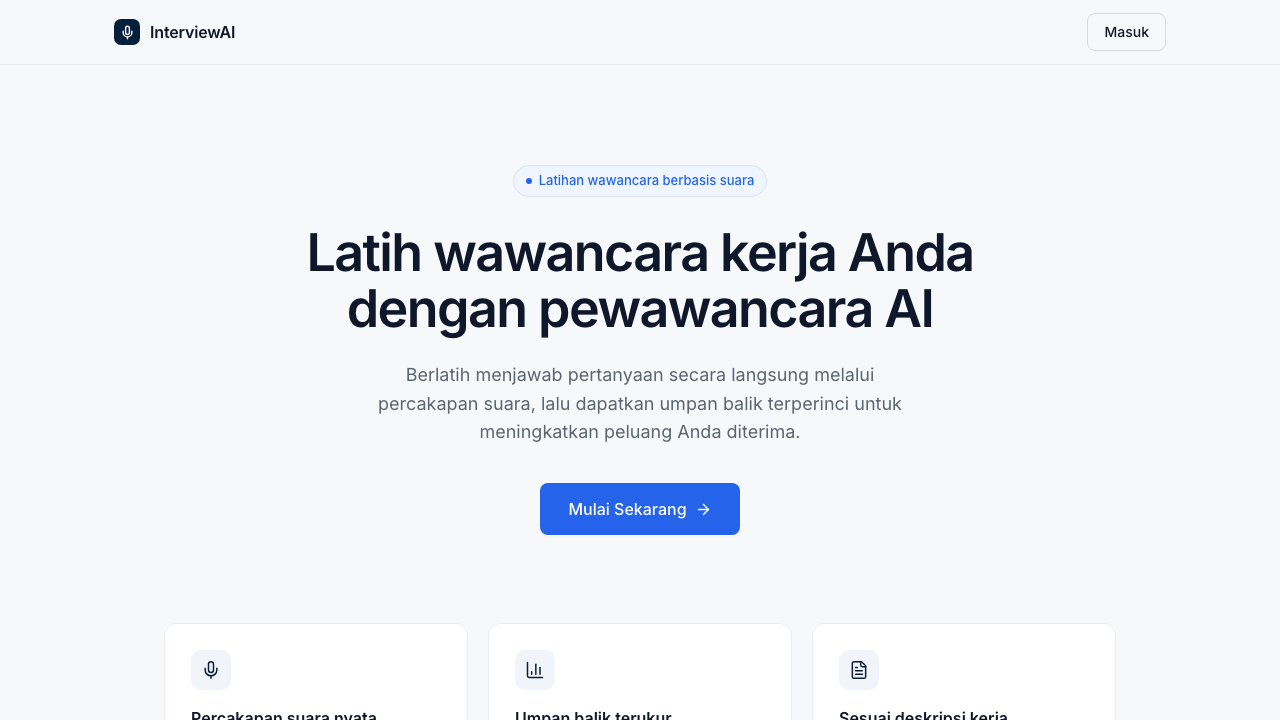
\includegraphics[width=\textwidth]{01-landing.png}
\caption{Halaman Landing}
\label{fig:landing}
\end{figure}

\begin{figure}[H]
\centering
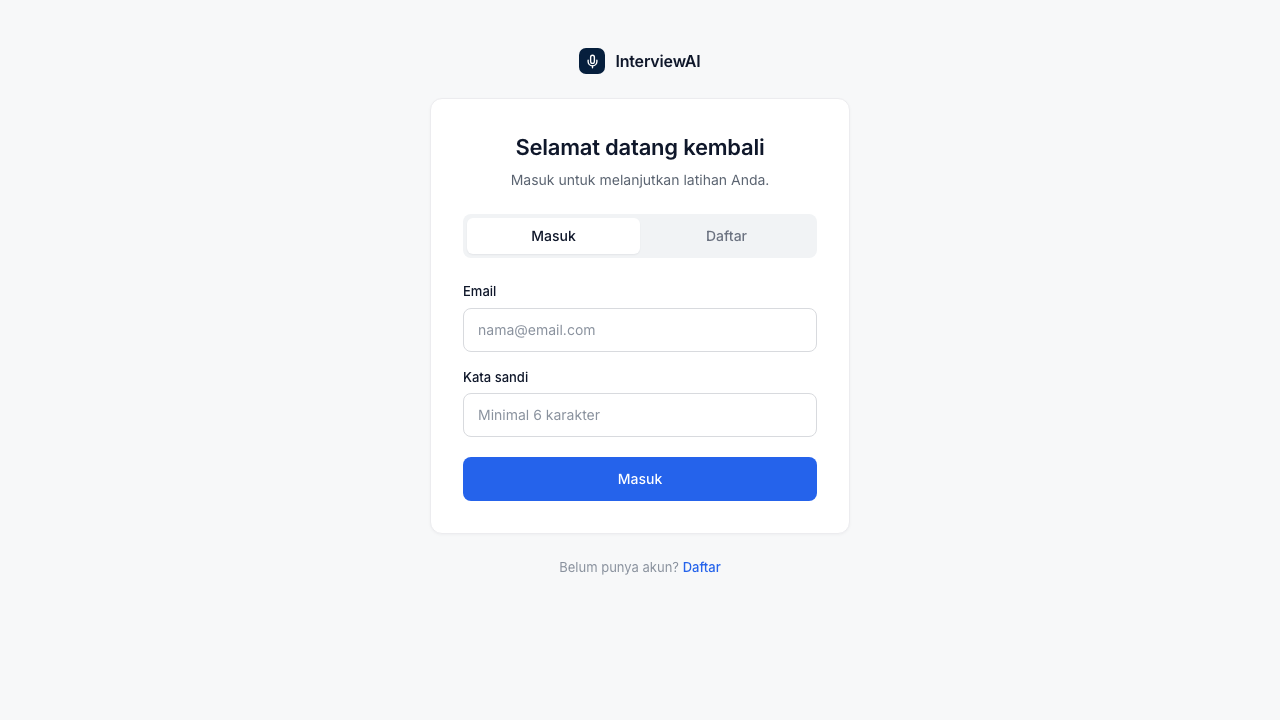
\includegraphics[width=0.8\textwidth]{02-login.png}
\caption{Halaman Login}
\label{fig:login}
\end{figure}

\begin{figure}[H]
\centering
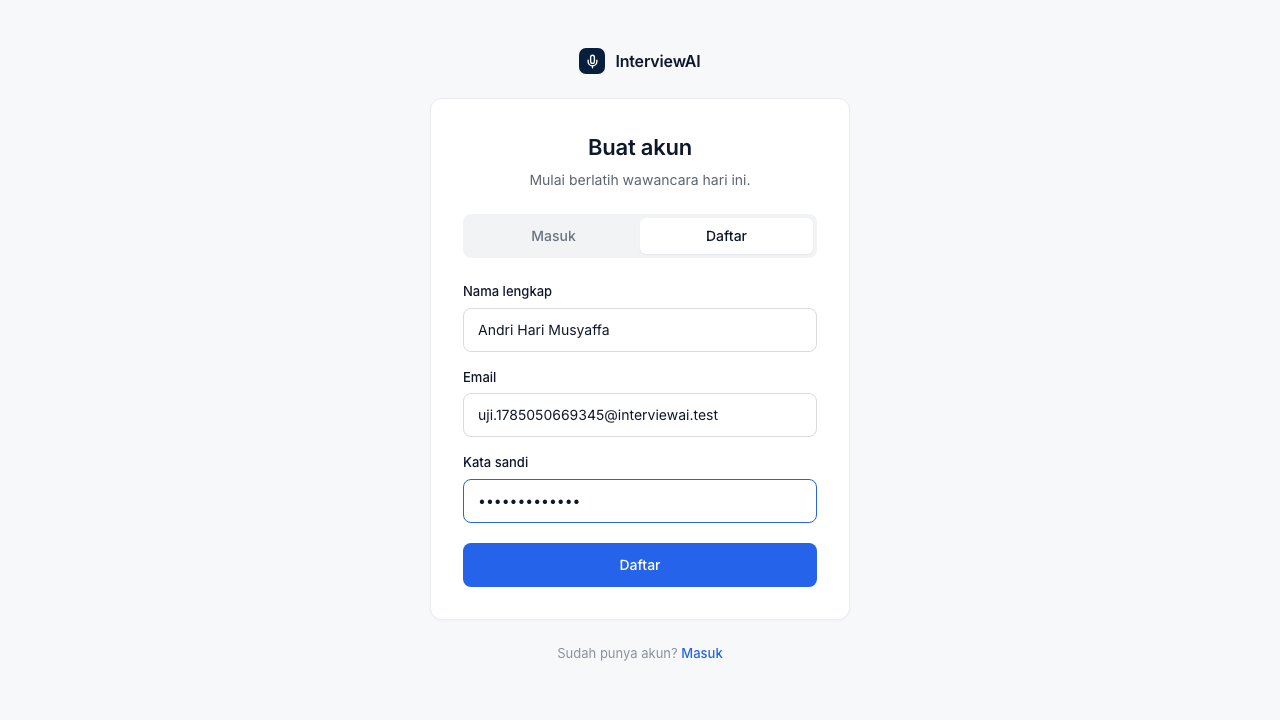
\includegraphics[width=0.8\textwidth]{03-register.png}
\caption{Halaman Register}
\label{fig:register}
\end{figure}

\begin{figure}[H]
\centering
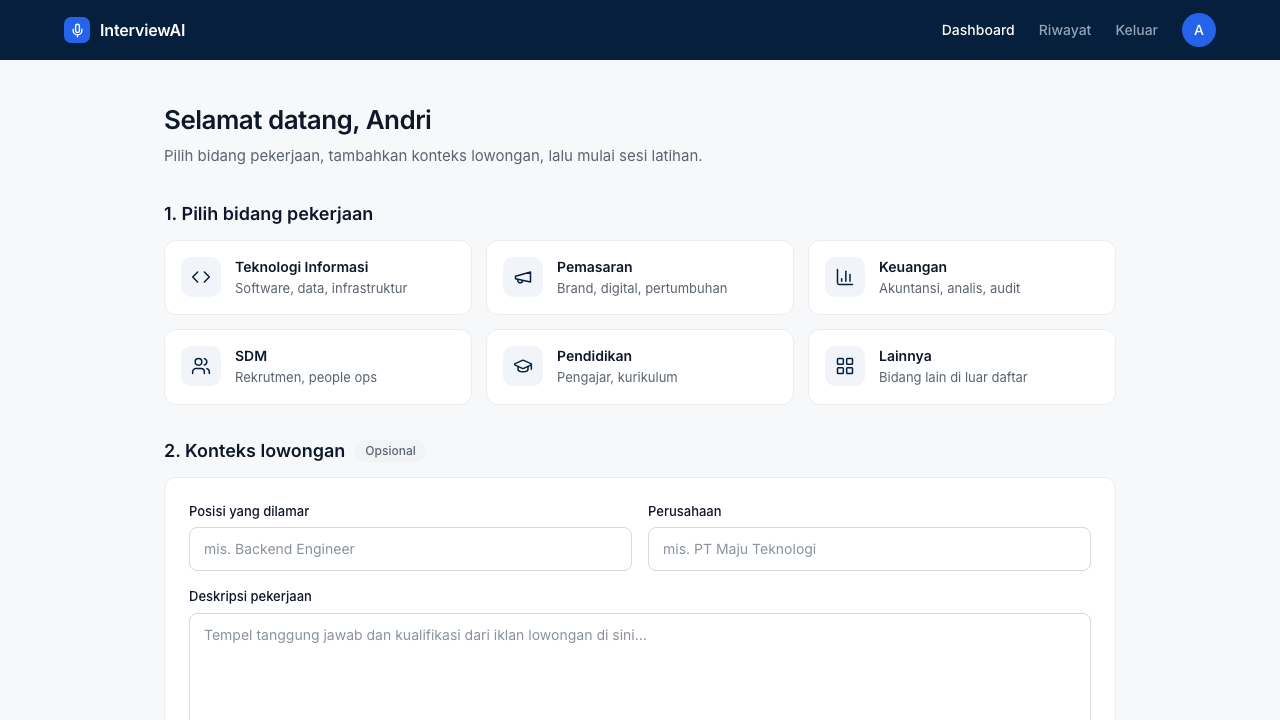
\includegraphics[width=\textwidth]{04-dashboard.png}
\caption{Halaman Dashboard --- Pemilihan Bidang Pekerjaan}
\label{fig:dashboard}
\end{figure}

\begin{figure}[H]
\centering
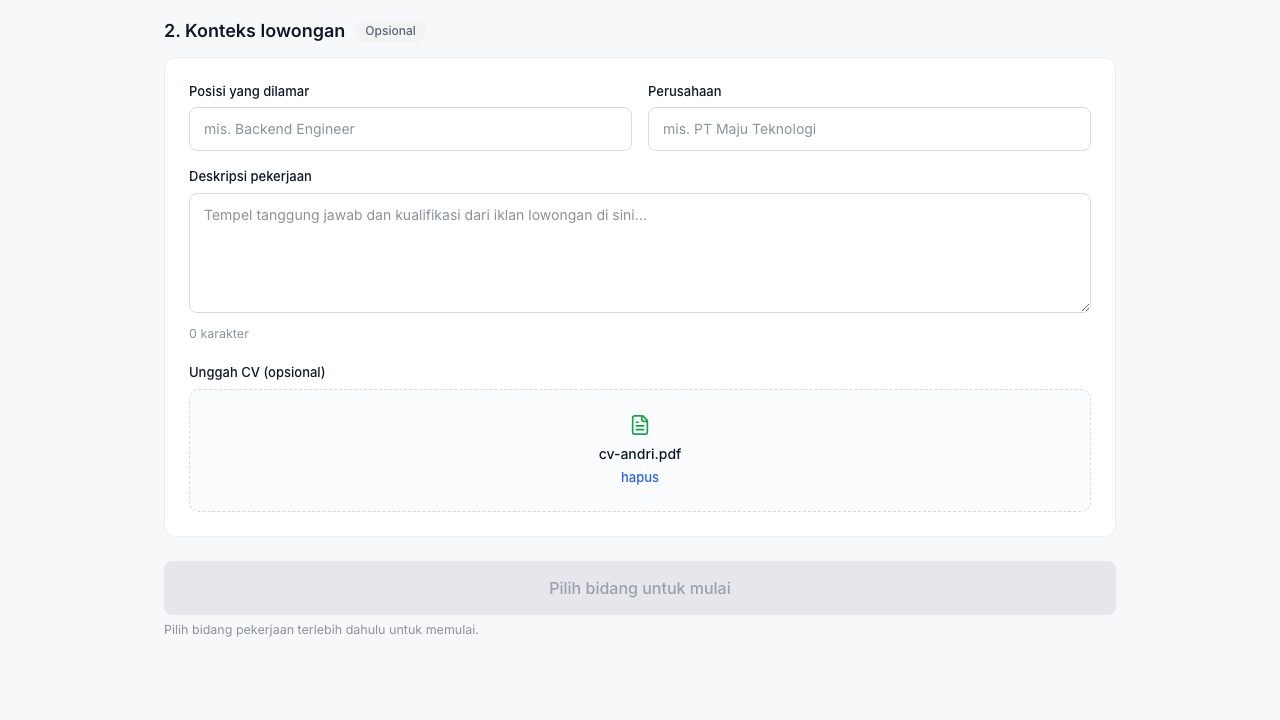
\includegraphics[width=\textwidth]{05-upload-cv.png}
\caption{Formulir Konteks Lowongan dan Unggah CV}
\label{fig:upload-cv}
\end{figure}

\begin{figure}[H]
\centering
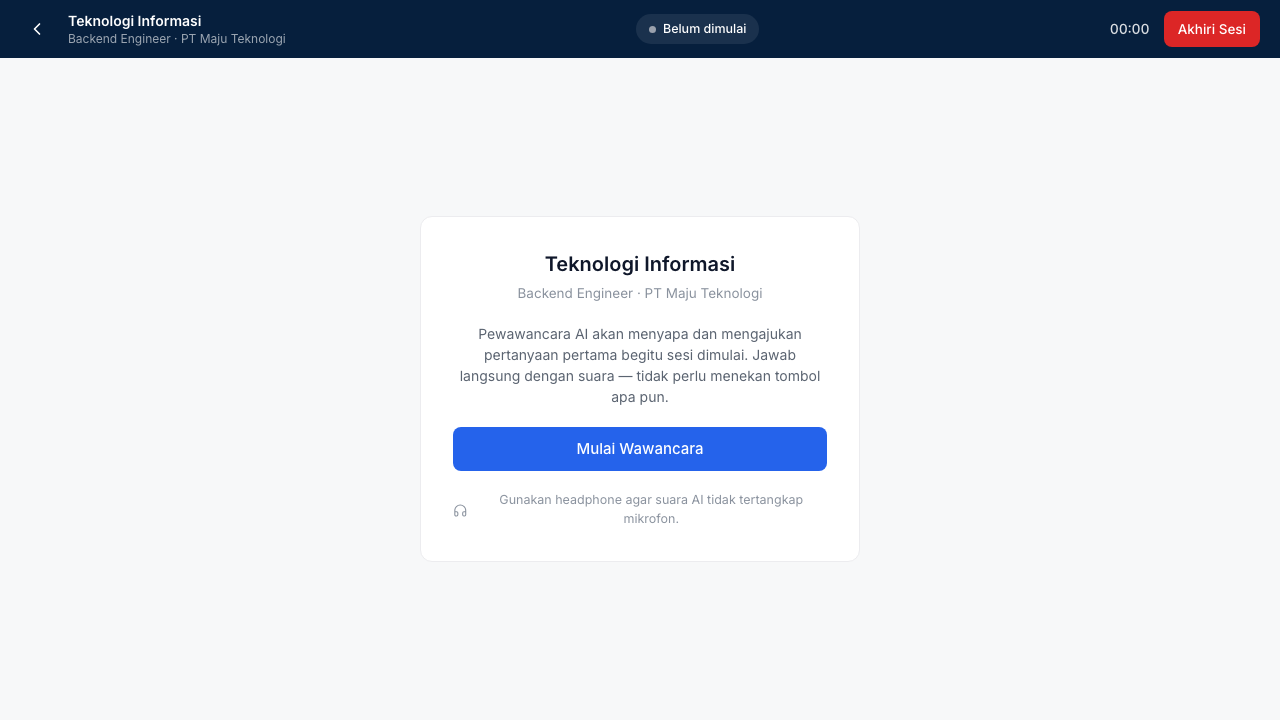
\includegraphics[width=\textwidth]{06-pre-session.png}
\caption{Halaman Persiapan Sesi Wawancara}
\label{fig:pre-session}
\end{figure}

\begin{figure}[H]
\centering
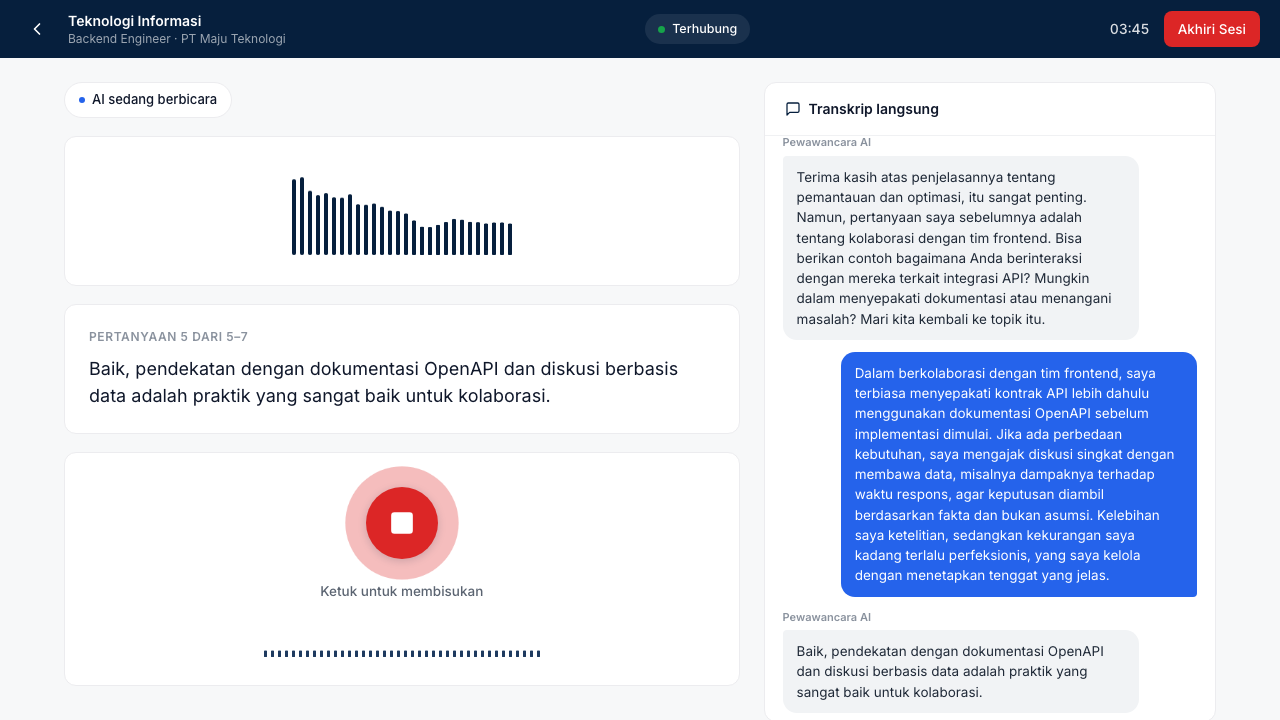
\includegraphics[width=\textwidth]{07-session-live.png}
\caption{Halaman Sesi Wawancara Berlangsung}
\label{fig:session-live}
\end{figure}

Gambar~\ref{fig:session-live} memperlihatkan sesi wawancara yang sedang
berjalan. Kolom kiri menampilkan indikator status pembicara, visualisasi
amplitudo audio, kartu pertanyaan terakhir, dan kendali mikrofon; sedangkan
kolom kanan menampilkan transkrip percakapan secara berurutan. Indikator
``Terhubung'' pada bilah atas menandakan koneksi \textit{WebSocket} ke Gemini
Live API dalam keadaan aktif, dan penghitung waktu menunjukkan durasi sesi
yang sedang berjalan.

\begin{figure}[H]
\centering
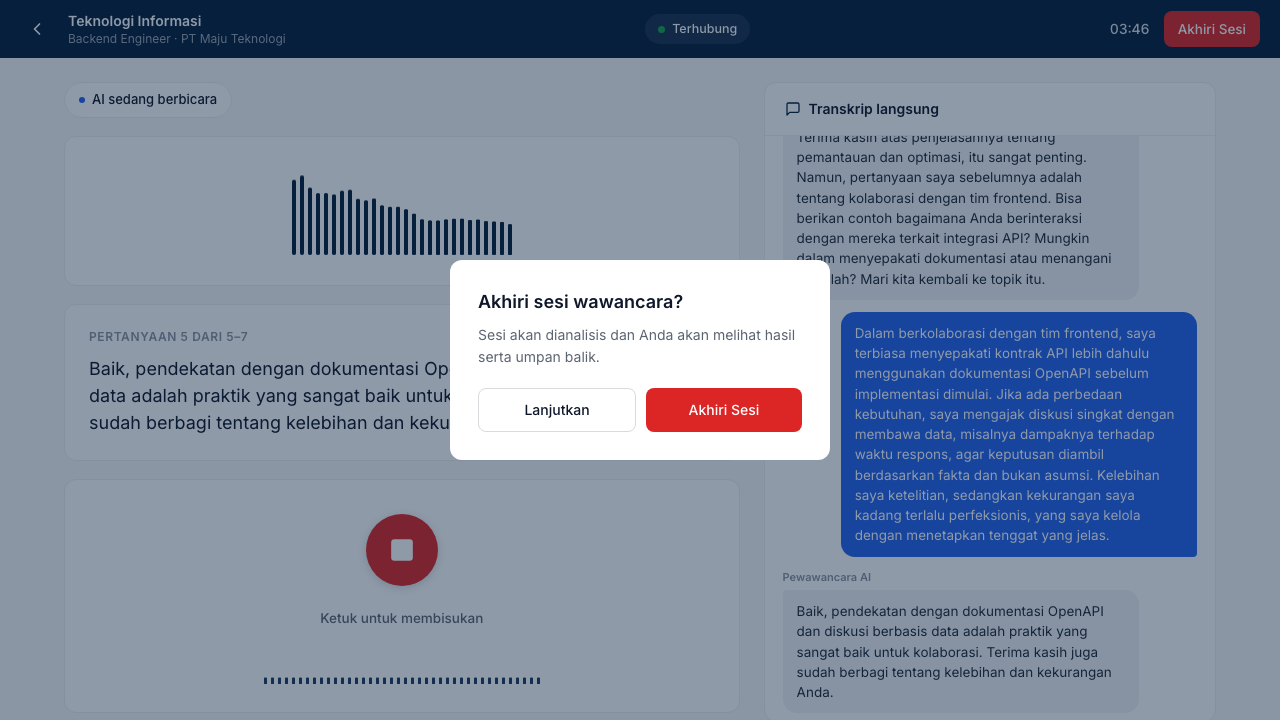
\includegraphics[width=\textwidth]{08-end-confirm.png}
\caption{Dialog Konfirmasi Pengakhiran Sesi}
\label{fig:end-confirm}
\end{figure}

\begin{figure}[H]
\centering
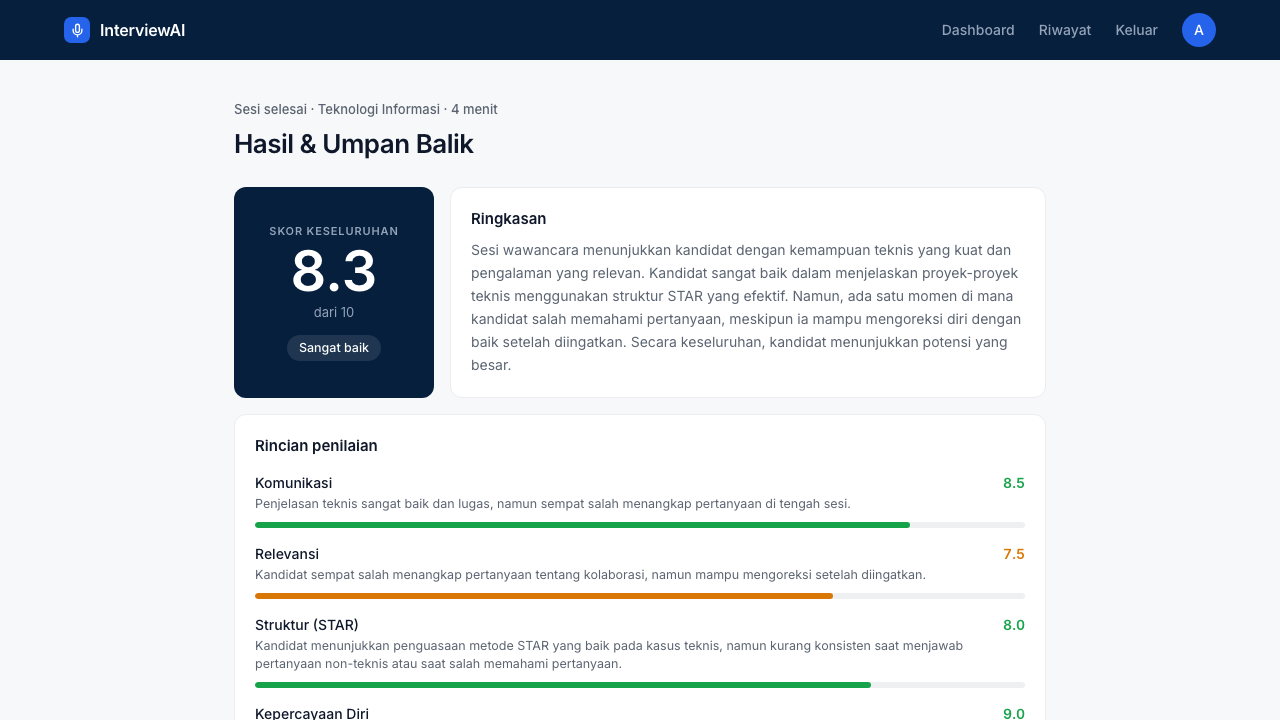
\includegraphics[width=\textwidth]{09-result.png}
\caption{Halaman Hasil dan Umpan Balik}
\label{fig:result}
\end{figure}

\begin{figure}[H]
\centering
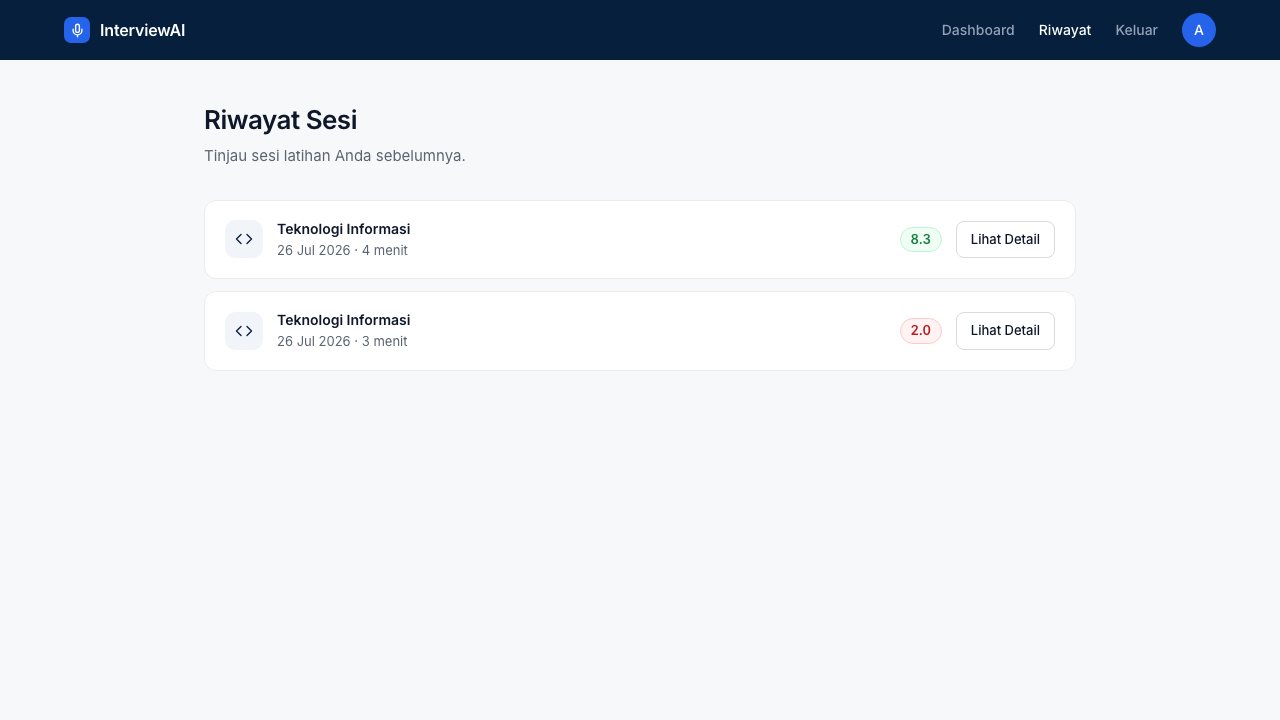
\includegraphics[width=\textwidth]{10-history.png}
\caption{Halaman Riwayat Sesi}
\label{fig:history}
\end{figure}

\begin{figure}[H]
\centering
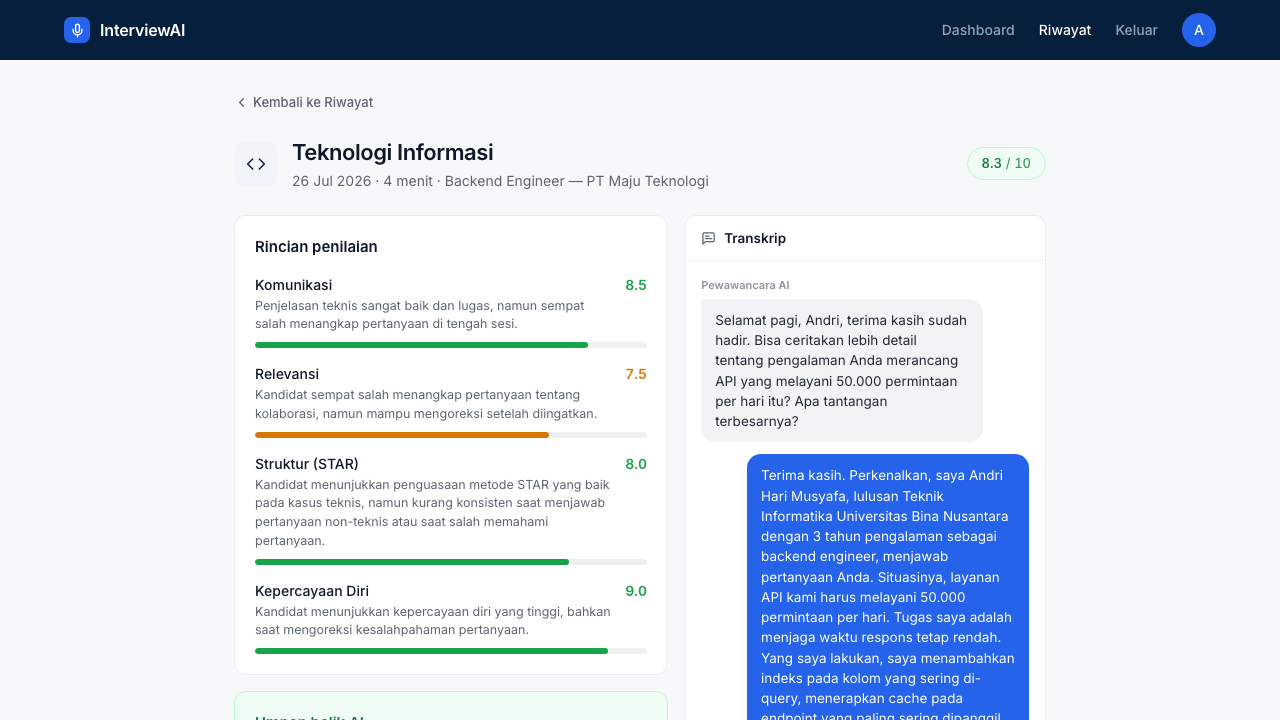
\includegraphics[width=\textwidth]{11-history-detail.png}
\caption{Halaman Detail Riwayat Sesi}
\label{fig:history-detail}
\end{figure}

\subsection{Implementasi Integrasi Gemini Live API}

Integrasi dengan Gemini Live API merupakan bagian paling kompleks dari sistem
ini karena melibatkan komunikasi audio dua arah secara \textit{real-time}.
Implementasinya menerapkan pola \textit{token broker}, yaitu \textit{backend}
tidak meneruskan aliran audio, melainkan hanya menerbitkan
\textit{ephemeral token} berumur pendek yang kemudian digunakan peramban untuk
membuka koneksi \textit{WebSocket Secure} langsung ke Gemini.

Alur satu sesi wawancara berjalan sebagai berikut:

\begin{enumerate}[leftmargin=*,itemsep=2pt]
  \item Pengguna memilih bidang pekerjaan, mengisi konteks lowongan, dan
        secara opsional mengunggah CV, lalu sistem membuat data sesi melalui
        \texttt{POST /api/sessions}.
  \item Peramban meminta \textit{ephemeral token} melalui
        \texttt{POST /api/sessions/:id/token}. Pada titik inilah
        \textit{backend} menyusun \textit{system instruction} yang berisi
        persona pewawancara beserta konteks sesi dan teks CV, lalu menguncinya
        di sisi server melalui \texttt{liveConnectConstraints}.
  \item Peramban membuka koneksi \textit{WebSocket} langsung ke Gemini
        menggunakan token tersebut, lalu mengirimkan perintah pembuka agar AI
        menyapa dan langsung mengajukan pertanyaan pertama.
  \item Audio mikrofon direkam pada 16 kHz, dikonversi menjadi PCM 16-bit di
        dalam \textit{AudioWorklet}, dan dikirimkan secara terus-menerus.
        Balasan audio Gemini pada 24 kHz diantrikan dan diputar kembali.
  \item Ketika pengguna mengakhiri sesi, transkrip dikirim ke
        \texttt{POST /api/sessions/}\linebreak[1]\texttt{:id/analyze} untuk dievaluasi, kemudian
        \texttt{POST /api/sessions/:id/end} menuliskan transkrip ke MongoDB
        lebih dahulu sebelum menandai sesi sebagai selesai di PostgreSQL.
\end{enumerate}

Parameter konfigurasi Gemini Live API hasil implementasi ditunjukkan pada
Tabel~\ref{tab:param-live}.

\begin{table}[H]
\caption{Parameter Konfigurasi Gemini Live API Hasil Implementasi}
\label{tab:param-live}
\centering
\begin{tabularx}{\textwidth}{|L{3.4cm}|L{4.2cm}|X|}
\hline
\textbf{Parameter} & \textbf{Nilai} & \textbf{Keterangan} \\
\hline
\textit{Model} & \texttt{gemini-3.1-flash-}\linebreak\texttt{live-preview} & Model \textit{native audio} dengan latensi terendah yang tersedia \\
\hline
Versi API & \texttt{v1alpha} & Versi yang menyediakan \textit{ephemeral token} \\
\hline
\textit{Response modalities} & \texttt{AUDIO} & Keluaran utama berupa audio \\
\hline
Transkripsi & \textit{input} dan \textit{output} diaktifkan & Menghasilkan transkrip dua arah untuk layar dan evaluasi \\
\hline
Format audio masuk & PCM 16-bit, 16 kHz, mono & Format yang diminta Gemini Live API \\
\hline
Format audio keluar & PCM 16-bit, 24 kHz, mono & Format balasan Gemini \\
\hline
\textit{Language code} & \texttt{id-ID} & Bahasa Indonesia \\
\hline
\textit{Voice} & \texttt{Kore} & Suara pewawancara AI \\
\hline
\textit{Temperature} & 0,7 & Keseimbangan variasi dan konsistensi respons \\
\hline
Masa berlaku token & 30 menit, sekali pakai & Membatasi dampak apabila token bocor \\
\hline
\end{tabularx}
\end{table}

\subsection{Implementasi Personalisasi Berbasis CV}

Berkas CV yang diunggah dalam format PDF maupun DOCX diekstraksi teksnya di
sisi \textit{backend}, lalu disisipkan ke dalam \textit{system instruction}
dengan batas maksimum 8.000 karakter. Pembatasan ini diperlukan karena
\textit{prompt} yang terlalu panjang meningkatkan biaya token sekaligus
latensi pada setiap sesi.

Efektivitas personalisasi ini terbukti pada saat pengujian. CV yang digunakan
memuat butir pengalaman berupa perancangan layanan API yang melayani 50.000
permintaan per hari. Pertanyaan pertama yang diajukan pewawancara AI adalah:

\begin{quote}
\textit{``Selamat pagi, Andri, terima kasih sudah hadir. Bisa ceritakan lebih
detail tentang pengalaman Anda merancang API yang melayani 50.000 permintaan
per hari itu? Apa tantangan terbesarnya?''}
\end{quote}

Pertanyaan tersebut menyebut angka yang hanya terdapat di dalam berkas CV,
sehingga membuktikan bahwa teks CV benar-benar terekstraksi, tersisipkan ke
dalam \textit{system instruction}, dan digunakan oleh model untuk menyusun
pertanyaan yang personal.

\subsection{Implementasi Evaluasi Terstruktur}

Evaluasi tidak dihasilkan oleh model percakapan, melainkan oleh model teks
terpisah (\texttt{gemini-2.5-flash}) yang menerima seluruh transkrip sesi.
Model diminta mengembalikan keluaran JSON terstruktur melalui mekanisme
\textit{response schema}, dengan empat metrik tetap yaitu Komunikasi,
Relevansi, Struktur (STAR), dan Kepercayaan Diri.

Karena keluaran model bahasa tetap berpotensi menyimpang dari skema yang
diminta, hasilnya melewati proses normalisasi sebelum disimpan. Proses ini
mencocokkan metrik berdasarkan \textit{key} maupun \textit{label},
membatasi setiap skor pada rentang 0--100, serta mengisi nilai cadangan
apabila ada bagian yang kosong. Dengan demikian bentuk data evaluasi yang
diterima antarmuka selalu konsisten, meskipun respons model bervariasi.

\subsection{Implementasi Keamanan}

Aspek keamanan yang berhasil diimplementasikan dirangkum pada
Tabel~\ref{tab:keamanan}.

\begin{table}[H]
\caption{Mekanisme Keamanan yang Diimplementasikan}
\label{tab:keamanan}
\centering
\begin{tabularx}{\textwidth}{|L{4.4cm}|X|}
\hline
\textbf{Aspek} & \textbf{Implementasi} \\
\hline
Kerahasiaan kunci API & Kunci API Gemini hanya berada di \textit{backend}; peramban hanya menerima \textit{ephemeral token} sekali pakai berumur 30 menit \\
\hline
Integritas persona AI & Model, \textit{system instruction}, suara, dan \textit{temperature} dikunci di sisi server; klien hanya boleh mengirim \textit{session resumption handle} \\
\hline
Autentikasi & JWT \textit{access token} berumur 15 menit dan \textit{refresh token} 7 hari pada \textit{cookie} \texttt{httpOnly} \\
\hline
Penyimpanan kata sandi & \textit{Hashing} menggunakan algoritma Argon2 \\
\hline
Pembatasan laju & 20 permintaan per IP tiap 15 menit pada \textit{endpoint} autentikasi, dan 40 permintaan per pengguna tiap 15 menit pada \textit{endpoint} yang memanggil Gemini \\
\hline
Otorisasi data & Setiap akses sesi maupun CV memverifikasi kepemilikan \texttt{user\_id}, dan parameter UUID divalidasi sebelum menyentuh basis data \\
\hline
Pengerasan HTTP & \textit{Helmet}, CORS dengan satu \textit{origin} dari variabel lingkungan, serta validasi variabel lingkungan saat proses \textit{boot} \\
\hline
\end{tabularx}
\end{table}

Pembatasan peran juga diterapkan pada tingkat \textit{prompt}. \textit{System
instruction} secara eksplisit melarang AI menjawab pertanyaan di luar konteks
wawancara serta mengabaikan permintaan untuk berganti peran atau membocorkan
isi instruksi, sebagai mitigasi terhadap upaya \textit{prompt injection}.

% =====================================================================
\section{Penyesuaian terhadap Rancangan BAB III}
% =====================================================================

Selama tahap implementasi ditemukan sejumlah kendala teknis yang menyebabkan
beberapa keputusan rancangan pada BAB III perlu disesuaikan. Ringkasan
penyesuaian tersebut ditunjukkan pada Tabel~\ref{tab:deviasi}, sedangkan
penyesuaian yang paling berdampak diuraikan pada sub-bab berikutnya.

\begin{table}[H]
\caption{Ringkasan Penyesuaian Rancangan terhadap Implementasi}
\label{tab:deviasi}
\centering
\begin{tabularx}{\textwidth}{|L{3.5cm}|L{3.4cm}|X|}
\hline
\textbf{Rancangan (BAB III)} & \textbf{Implementasi} & \textbf{Alasan Penyesuaian} \\
\hline
Supabase sebagai penyedia PostgreSQL, Auth, dan Storage & PostgreSQL mandiri, autentikasi JWT + Argon2 sendiri, CV disimpan pada \textit{filesystem} server & Menghilangkan ketergantungan pada layanan pihak ketiga dan biaya berlangganan, sekaligus memberi kendali penuh atas skema basis data dan masa berlaku token \\
\hline
\textit{Backend} berperan sebagai \textit{WebSocket proxy} & Pola \textit{token broker}; audio mengalir langsung dari peramban ke Gemini & \textit{Proxy} menambah satu lompatan jaringan pada jalur yang paling sensitif terhadap latensi dan membebani server dengan seluruh aliran audio. Pola \textit{token broker} tetap menjaga kerahasiaan kunci API tanpa biaya latensi tersebut \\
\hline
Model \texttt{gemini-live-}\linebreak\texttt{3-flash}, suara bawaan & \texttt{gemini-3.1-}\linebreak\texttt{flash-live-}\linebreak\texttt{preview}, suara \texttt{Kore}, \texttt{id-ID} & Nama model pada rancangan tidak tersedia. Model yang dipilih memberi waktu respons sekitar 1,5 detik dibanding sekitar 5,0 detik pada alternatifnya \\
\hline
Evaluasi berupa \texttt{overall\_score} dan \texttt{feedback\_text} & Ditambah empat metrik terstruktur, \texttt{strengths}, \texttt{improvements}, dan \texttt{summary} & Skor tunggal tidak cukup informatif sebagai bahan perbaikan. Penilaian per aspek menjawab kebutuhan umpan balik yang dapat ditindaklanjuti \\
\hline
Tipe kunci utama pada \texttt{job\_fields} adalah SERIAL & Bertipe UUID & Menyeragamkan tipe kunci seluruh tabel sehingga tidak ada identitas yang mudah ditebak berurutan \\
\hline
\textit{Deployment} pada Vercel dan Cloud Run & Direncanakan pada VPS di belakang \textit{nginx} & Menyederhanakan operasional menjadi satu lingkungan dan menekan biaya. Tahap ini belum dilaksanakan pada penelitian ini \\
\hline
\end{tabularx}
\end{table}

\subsection{Penggantian Supabase dengan Layanan Mandiri}

Rancangan awal menempatkan Supabase sebagai penyedia PostgreSQL, autentikasi,
dan penyimpanan berkas sekaligus. Pada implementasi, ketiga peran tersebut
dipisahkan dan dikelola sendiri. PostgreSQL dijalankan secara mandiri dengan
skema yang dikelola melalui berkas migrasi SQL berurutan, autentikasi
diimplementasikan menggunakan JWT dengan \textit{hashing} Argon2, dan berkas
CV disimpan pada \textit{filesystem} server dengan nama berkas yang diacak.

Konsekuensinya, pengelolaan keamanan autentikasi menjadi tanggung jawab
sistem ini sendiri. Hal tersebut dikompensasi dengan penerapan \textit{refresh
token} pada \textit{cookie} \texttt{httpOnly}, masa berlaku \textit{access
token} yang pendek, serta pembatasan laju pada \textit{endpoint}
autentikasi.

\subsection{Perubahan Pola Integrasi menjadi \textit{Token Broker}}

Perubahan paling mendasar terjadi pada pola integrasi dengan Gemini Live API.
Rancangan BAB III menempatkan \textit{backend} sebagai \textit{WebSocket
proxy} yang meneruskan audio dari klien ke Gemini. Pendekatan tersebut
memiliki dua kelemahan: seluruh aliran audio dua arah harus melewati server
sehingga menambah beban dan biaya bandwidth, dan setiap lompatan tambahan
menambah latensi pada jalur yang justru paling menentukan kealamian
percakapan.

Pada implementasi, \textit{backend} hanya berperan menerbitkan
\textit{ephemeral token}, sedangkan koneksi \textit{WebSocket} dibuka langsung
dari peramban ke Gemini. Kerahasiaan kunci API tetap terjaga karena kunci
tersebut tidak pernah meninggalkan server, dan konfigurasi sesi dikunci pada
saat token diterbitkan sehingga klien tidak dapat mengubah persona
pewawancara, model, maupun suara yang digunakan.

\subsection{Perluasan Skema Evaluasi}

Rancangan awal hanya menyimpan skor keseluruhan dan umpan balik naratif.
Skema tersebut diperluas menjadi empat metrik penilaian beserta catatannya,
ditambah daftar kelebihan, daftar hal yang perlu ditingkatkan, dan ringkasan
sesi. Perluasan ini menjawab tujuan penelitian mengenai umpan balik yang
bersifat personal, karena pengguna dapat mengetahui aspek mana yang lemah dan
bukan sekadar menerima satu angka.

% =====================================================================
\section{Pengujian Sistem}
% =====================================================================

\subsection{Metode dan Lingkungan Pengujian}

Pengujian dilakukan menggunakan metode \textit{Black Box Testing} sesuai
rencana pada BAB III, yaitu memvalidasi fungsionalitas berdasarkan masukan dan
keluaran yang diharapkan tanpa memeriksa struktur internal kode program.
Seluruh skenario diotomasi menggunakan Playwright dan dijalankan pada peramban
Chromium, sehingga pengujian dapat diulang dan hasilnya dapat diverifikasi
kembali.

Skenario dijalankan secara berurutan dalam satu \textit{worker} karena antar
skenario terdapat ketergantungan data: sesi wawancara yang diselesaikan pada
berkas skenario ketiga merupakan data yang diperiksa oleh skenario pengujian
riwayat. Dengan demikian alur simpan dan baca lintas kedua basis data ikut
terverifikasi.

Pengujian sesi wawancara suara memerlukan sumber suara kandidat. Suara
tersebut disintesis menggunakan \textit{text-to-speech} berbahasa Indonesia
berisi lima jawaban yang disusun mengikuti kerangka STAR, dengan jeda hening
di antara jawaban agar giliran bicara tidak bertabrakan dengan suara
pewawancara AI.

Pada tahap penyiapan ditemukan bahwa opsi Chromium
\texttt{-{}-use-file-for-}\allowbreak\texttt{fake-audio-capture} tidak berpengaruh pada
lingkungan pengujian yang digunakan. Hal ini diverifikasi menggunakan berkas
uji berpola nada keras dan hening bergantian setiap satu detik: pola tersebut
sama sekali tidak muncul pada data PCM yang benar-benar dikirimkan aplikasi ke
Gemini. Oleh karena itu mikrofon disimulasikan satu lapis lebih tinggi, yaitu
dengan mengembalikan \textit{MediaStream} yang dibangkitkan Web Audio API dari
berkas suara yang sama. Yang disimulasikan hanya perangkat keras mikrofonnya,
sedangkan seluruh jalur kode aplikasi --- \textit{AudioWorklet}, konversi PCM
16 kHz, hingga pengiriman ke Gemini --- tetap berjalan apa adanya, sehingga
pengujian tetap sah sebagai pengujian \textit{Black Box} terhadap sistem.

\subsection{Skenario dan Hasil Pengujian}

Sebanyak 26 skenario pengujian disusun untuk mencakup kesebelas
\textit{use case} yang dirancang pada BAB III, mencakup kasus normal maupun
kasus negatif. Hasil pengujian selengkapnya ditunjukkan pada
Tabel~\ref{tab:hasil-uji}.

\begin{longtable}{|C{1.1cm}|C{1.1cm}|L{4.5cm}|L{3.1cm}|C{1.3cm}|}
\caption{Hasil Pengujian \textit{Black Box}}
\label{tab:hasil-uji} \\
\hline
\textbf{Kode} & \textbf{UC} & \textbf{Skenario Pengujian} & \textbf{Hasil yang Diharapkan} & \textbf{Hasil} \\
\hline
\endfirsthead
\multicolumn{5}{l}{\small\textit{Lanjutan Tabel \ref{tab:hasil-uji}}} \\
\hline
\textbf{Kode} & \textbf{UC} & \textbf{Skenario Pengujian} & \textbf{Hasil yang Diharapkan} & \textbf{Hasil} \\
\hline
\endhead
\hline
\endfoot
\hline
\endlastfoot

TC-00 & -- & Membuka halaman Landing & Judul dan tombol ``Mulai Sekarang'' tampil & Valid \\
\hline
TC-01 & UC-02 & Membuka Dashboard tanpa autentikasi & Dialihkan ke halaman Login & Valid \\
\hline
TC-02 & UC-01 & Register dengan format email tidak valid & Pesan ``Masukkan email yang valid'' tampil & Valid \\
\hline
TC-03 & UC-01 & Register dengan kata sandi kurang dari 6 karakter & Pesan ``Kata sandi minimal 6 karakter'' tampil & Valid \\
\hline
TC-04 & UC-01 & Register dengan data lengkap dan valid & Akun terbentuk dan masuk ke Dashboard & Valid \\
\hline
TC-05 & UC-01 & Register dengan email yang sudah terdaftar & Ditolak server dengan pesan galat & Valid \\
\hline
TC-06 & UC-02 & Login dengan kata sandi salah & Ditolak dan tetap di halaman Login & Valid \\
\hline
TC-07 & UC-02 & Login dengan kredensial benar & Masuk ke Dashboard & Valid \\
\hline
TC-08 & UC-10 & Menekan tombol Keluar & Sesi berakhir dan halaman terproteksi diblokir & Valid \\
\hline
TC-09 & UC-03 & Memuat daftar bidang pekerjaan & Enam bidang pekerjaan tampil dari server & Valid \\
\hline
TC-10 & UC-03 & Belum memilih bidang pekerjaan & Tombol mulai sesi dalam keadaan nonaktif & Valid \\
\hline
TC-11 & UC-03 & Memilih salah satu bidang pekerjaan & Tombol mulai sesi menjadi aktif & Valid \\
\hline
TC-12 & UC-03 & Mengisi deskripsi lowongan lebih dari 40 karakter & Konfirmasi ``Konteks akan dipakai AI'' tampil & Valid \\
\hline
TC-13 & UC-11 & Mengunggah CV berformat PDF & Berkas terunggah dan teksnya terekstraksi & Valid \\
\hline
TC-14 & UC-11 & Mengunggah CV berformat DOCX & Berkas terunggah dan teksnya terekstraksi & Valid \\
\hline
TC-15 & UC-11 & Mengunggah berkas berformat selain PDF/DOCX & Ditolak dengan pesan format tidak sesuai & Valid \\
\hline
TC-16 & UC-11 & Menghapus CV yang telah diunggah & Formulir kembali ke keadaan semula & Valid \\
\hline
TC-17 & UC-04 & Menekan tombol Mulai Sesi Wawancara & Sesi terbentuk dan halaman wawancara terbuka & Valid \\
\hline
TC-18 & UC-04 & Memulai wawancara & Koneksi terbuka dan AI menyapa serta bertanya & Valid \\
\hline
TC-19 & UC-05 & Kandidat menjawab dengan suara & Jawaban tertranskripsi pada panel transkrip & Valid \\
\hline
TC-20 & UC-06 & Melanjutkan percakapan beberapa giliran & AI menanggapi jawaban dan mengajukan pertanyaan lanjutan & Valid \\
\hline
TC-21 & UC-07 & Mengakhiri sesi wawancara & Evaluasi dihasilkan dan halaman Hasil tampil lengkap & Valid \\
\hline
TC-22 & UC-08 & Membuka halaman Riwayat & Sesi yang telah selesai tampil beserta skornya & Valid \\
\hline
TC-23 & UC-09 & Membuka detail salah satu sesi & Rincian penilaian dan transkrip tampil & Valid \\
\hline
TC-24 & UC-09 & Membuka detail sesi milik pengguna lain & Akses ditolak dan pesan galat tampil & Valid \\
\hline
TC-25 & UC-09 & Kembali dari detail ke daftar riwayat & Kembali ke halaman Riwayat & Valid \\
\hline
\end{longtable}

\subsection{Analisis Persentase Keberhasilan}

Persentase keberhasilan dihitung menggunakan rumus yang telah ditetapkan pada
BAB III, yaitu:

\begin{center}
\textit{Success Rate} $=\dfrac{\text{Jumlah \textit{test case} valid}}{\text{Total \textit{test case}}}\times 100\%$
\end{center}

Rekapitulasi hasil pengujian per \textit{use case} ditunjukkan pada
Tabel~\ref{tab:success-rate}.

\begin{table}[H]
\caption{Rekapitulasi Persentase Keberhasilan per \textit{Use Case}}
\label{tab:success-rate}
\centering
\begin{tabularx}{\textwidth}{|C{1.6cm}|X|C{1.9cm}|C{1.6cm}|C{2.1cm}|}
\hline
\textbf{Kode UC} & \textbf{Nama \textit{Use Case}} & \textbf{Jumlah \textit{Test Case}} & \textbf{Valid} & \textbf{Persentase} \\
\hline
UC-01 & Register & 4 & 4 & 100\% \\
\hline
UC-02 & Login & 3 & 3 & 100\% \\
\hline
UC-03 & Memilih Bidang Pekerjaan & 4 & 4 & 100\% \\
\hline
UC-04 & Memulai Sesi Wawancara & 2 & 2 & 100\% \\
\hline
UC-05 & Menjawab Pertanyaan & 1 & 1 & 100\% \\
\hline
UC-06 & Menerima Umpan Balik & 1 & 1 & 100\% \\
\hline
UC-07 & Mengakhiri Sesi & 1 & 1 & 100\% \\
\hline
UC-08 & Melihat Riwayat Sesi & 1 & 1 & 100\% \\
\hline
UC-09 & Melihat Detail Riwayat & 3 & 3 & 100\% \\
\hline
UC-10 & Logout & 1 & 1 & 100\% \\
\hline
UC-11 & Mengunggah CV & 4 & 4 & 100\% \\
\hline
-- & Umum (halaman Landing) & 1 & 1 & 100\% \\
\hline
\multicolumn{2}{|c|}{\textbf{Total}} & \textbf{26} & \textbf{26} & \textbf{100\%} \\
\hline
\end{tabularx}
\end{table}

Berdasarkan rekapitulasi tersebut, seluruh 26 \textit{test case} dinyatakan
valid sehingga persentase keberhasilan mencapai 100\%. Nilai ini melampaui
ambang minimal 90\% untuk setiap kategori fitur yang ditetapkan pada BAB III,
sehingga hipotesis penelitian mengenai keberhasilan fungsional sistem
dinyatakan terpenuhi.

% =====================================================================
\section{Pembahasan}
% =====================================================================

\subsection{Ketercapaian Tujuan Penelitian}

Rumusan masalah pertama mempertanyakan bagaimana merancang dan membangun
\textit{website} simulasi wawancara kerja berbasis \textit{Large Language
Model} dengan memanfaatkan Gemini Live API. Hasil implementasi menunjukkan
bahwa sistem tersebut berhasil dibangun secara utuh, mulai dari autentikasi,
konfigurasi sesi, wawancara suara \textit{real-time}, evaluasi otomatis,
hingga riwayat sesi. Sistem berjalan sepenuhnya di dalam peramban tanpa
memerlukan pemasangan perangkat lunak tambahan, dan seluruh antarmukanya
menggunakan Bahasa Indonesia sehingga dapat diakses oleh pencari kerja di
Indonesia tanpa hambatan bahasa maupun biaya sesi.

Rumusan masalah kedua mempertanyakan bagaimana mengintegrasikan fitur
pertanyaan otomatis, penilaian jawaban, umpan balik personal, dan komunikasi
suara \textit{real-time} ke dalam satu \textit{platform} berbasis web.
Keempat fitur tersebut terbukti berjalan dalam satu alur yang berkesinambungan
sebagaimana ditunjukkan pada pengujian TC-17 sampai TC-21. Pertanyaan
dihasilkan secara otomatis dan dipersonalisasi berdasarkan CV, jawaban
disampaikan melalui suara dan tertranskripsi, umpan balik lisan diberikan di
sela percakapan, serta penilaian tertulis per aspek disajikan setelah sesi
berakhir.

\subsection{Analisis Kinerja Percakapan \textit{Real-time}}

Pengukuran kinerja diambil langsung pada saat pengujian sesi wawancara
berlangsung dan dirangkum pada Tabel~\ref{tab:kinerja}.

\begin{table}[H]
\caption{Hasil Pengukuran Kinerja Sesi Wawancara}
\label{tab:kinerja}
\centering
\begin{tabularx}{\textwidth}{|X|C{3cm}|}
\hline
\textbf{Aspek yang Diukur} & \textbf{Hasil} \\
\hline
Waktu dari penekanan tombol mulai hingga AI mengucapkan sapaan pertama & 2,2 detik \\
\hline
Waktu dari mulai berbicara hingga jawaban muncul pada panel transkrip & 58,1 detik\footnotemark \\
\hline
Jumlah giliran bicara pewawancara AI dalam satu sesi & 5 giliran \\
\hline
Jumlah giliran bicara kandidat dalam satu sesi & 4 giliran \\
\hline
Total panjang transkrip jawaban kandidat & 1.856 karakter \\
\hline
Waktu pembuatan evaluasi setelah sesi diakhiri & 11,9 detik \\
\hline
\end{tabularx}
\end{table}
\footnotetext{Angka ini mencakup jeda hening 17 detik pada awal berkas suara
uji dan durasi pengucapan jawaban itu sendiri, sehingga bukan merupakan
latensi transkripsi murni. Latensi transkripsi terukur berada pada kisaran 3
detik di belakang penutur.}

Waktu tanggap awal sebesar 2,2 detik menunjukkan bahwa pola \textit{token
broker} tidak menimbulkan penundaan yang terasa, meskipun peramban harus
meminta token ke \textit{backend} terlebih dahulu sebelum membuka koneksi ke
Gemini. Adapun waktu pembuatan evaluasi sebesar 11,9 detik masih dapat
diterima karena berlangsung sekali di akhir sesi dan disertai indikator
pemuatan pada antarmuka.

Karakteristik penting yang ditemukan pada tahap implementasi adalah bahwa
transkripsi masukan dari Gemini berjalan sekitar tiga detik di belakang
penutur. Akibatnya, indikator ``sedang berbicara'' pada antarmuka tidak dapat
mengandalkan transkrip tersebut. Sistem mengatasinya dengan mendeteksi
amplitudo suara secara lokal di peramban, dan sinyal tersebut digunakan
semata-mata untuk keperluan tampilan, tidak pernah untuk menggerbang
pengiriman audio ke Gemini.

\subsection{Analisis Kualitas Evaluasi}

Selama tahap pengujian dilakukan dua kali sesi wawancara dengan naskah jawaban
yang berbeda, dan perbandingan hasilnya ditunjukkan pada
Tabel~\ref{tab:banding-evaluasi}.

\begin{table}[H]
\caption{Perbandingan Hasil Evaluasi terhadap Dua Naskah Jawaban}
\label{tab:banding-evaluasi}
\centering
\begin{tabularx}{\textwidth}{|X|C{2.4cm}|C{2.4cm}|}
\hline
\textbf{Karakteristik Naskah Jawaban} & \textbf{Skor Keseluruhan} & \textbf{Skor Relevansi} \\
\hline
Jawaban umum yang tidak menanggapi pertanyaan spesifik pewawancara & 2,0 & 1,5 \\
\hline
Jawaban terstruktur STAR yang menanggapi pokok pertanyaan & 8,3 & tinggi \\
\hline
\end{tabularx}
\end{table}

Perbedaan skor yang lebar antara kedua naskah menunjukkan bahwa mekanisme
evaluasi bersifat diskriminatif, yaitu benar-benar menilai isi dan relevansi
jawaban dan bukan sekadar memberikan skor tinggi secara seragam. Pada naskah
pertama, sistem secara tepat mengidentifikasi bahwa kandidat berulang kali
tidak menjawab pertanyaan yang diajukan, dan hal tersebut tercermin pada skor
Relevansi yang rendah. Temuan ini memperkuat keyakinan bahwa umpan balik yang
dihasilkan sistem memiliki nilai diagnostik bagi pengguna.

\subsection{Keterbatasan Sistem}

Berdasarkan hasil implementasi dan pengujian, terdapat sejumlah keterbatasan
yang perlu dicatat:

\begin{enumerate}[leftmargin=*,itemsep=3pt]
  \item \textbf{Ketergantungan pada model \textit{preview}.} Model
        \texttt{gemini-3.1-flash-}\allowbreak\texttt{live-preview} berstatus
        \textit{preview}
        sehingga berpotensi berubah atau dihentikan sewaktu-waktu. Sistem
        belum memiliki mekanisme peralihan otomatis ke model cadangan.
  \item \textbf{Penentuan batas giliran bicara bersifat heuristik.} Karena
        Gemini tidak menyertakan penanda waktu pengucapan pada setiap potongan
        transkrip, sistem menentukan giliran berdasarkan waktu kedatangan
        data. Pada kondisi tertentu, beberapa kata terakhir sebuah jawaban
        dapat tergeser ke giliran berikutnya, meskipun isi dan urutan
        percakapan secara keseluruhan tetap terjaga.
  \item \textbf{Penilaian terbatas pada aspek verbal.} Sesuai ruang lingkup
        pada BAB III, sistem tidak menilai aspek psikologis maupun bahasa
        tubuh, karena masukannya hanya berupa suara.
  \item \textbf{Pengujian belum mencakup keberagaman pengguna nyata.}
        Pengujian dilakukan menggunakan suara sintetis pada satu lingkungan
        peramban. Variasi aksen, kecepatan bicara, kualitas mikrofon, dan
        kondisi kebisingan pengguna nyata belum terwakili.
  \item \textbf{Tahap \textit{deployment} belum dilaksanakan.} Sistem baru
        berjalan pada lingkungan pengembangan lokal, sehingga pengujian
        performa pada kondisi produksi belum dapat dilakukan.
\end{enumerate}

\end{document}
. Bila
% disisipkan, preamble di bawah diabaikan secara otomatis.
% =====================================================================
\documentclass[12pt,a4paper,oneside]{report}

\usepackage[T1]{fontenc}
\usepackage[utf8]{inputenc}
\usepackage{newtxtext,newtxmath}          % Times New Roman
\usepackage[bahasa]{babel}
\usepackage[a4paper,left=4cm,right=3cm,top=3cm,bottom=3cm]{geometry}
\usepackage{setspace}
\usepackage{graphicx}
\usepackage{array}
\usepackage{longtable}
\usepackage{tabularx}
\usepackage{ragged2e}
\usepackage{enumitem}
\usepackage{caption}
\usepackage{float}
\usepackage{titlesec}
\usepackage[hidelinks]{hyperref}

% Judul bab bergaya skripsi: "BAB IV" di atas, judul bab di bawahnya, keduanya
% rata tengah dan huruf kapital.
\titleformat{\chapter}[display]
  {\normalfont\bfseries\centering}
  {\Large BAB \Roman{chapter}}{12pt}{\Large}
\titlespacing*{\chapter}{0pt}{0pt}{28pt}

\graphicspath{{gambar/}}

% Judul tabel di atas, judul gambar di bawah, keduanya rata tengah dan tebal.
\captionsetup[table]{position=top,labelsep=space,font=bf,justification=centering}
\captionsetup[figure]{position=bottom,labelsep=space,font=bf,justification=centering}

\newcolumntype{L}[1]{>{\RaggedRight\arraybackslash}p{#1}}
\newcolumntype{C}[1]{>{\Centering\arraybackslash}p{#1}}

\setlength{\emergencystretch}{3em}

\setcounter{chapter}{3}   % bab berikutnya menjadi BAB IV
\onehalfspacing

\begin{document}

\chapter{HASIL DAN PEMBAHASAN}

Bab ini menyajikan hasil tahap implementasi dan tahap pengujian dari metode
pengembangan \textit{Waterfall} yang telah diuraikan pada BAB III. Pembahasan
dimulai dari lingkungan implementasi dan wujud sistem yang berhasil dibangun,
dilanjutkan dengan penjelasan mengenai penyesuaian yang dilakukan terhadap
rancangan awal beserta alasan teknisnya, kemudian hasil pengujian
\textit{Black Box} atas seluruh \textit{use case}, dan ditutup dengan
pembahasan mengenai ketercapaian tujuan penelitian serta keterbatasan sistem.

% =====================================================================
\section{Lingkungan Implementasi}
% =====================================================================

Sistem dibangun dan diuji pada lingkungan pengembangan dengan spesifikasi
sebagaimana ditunjukkan pada Tabel~\ref{tab:lingkungan}. Seluruh komponen
dijalankan secara lokal, kecuali layanan Gemini yang diakses melalui jaringan
internet.

\begin{table}[H]
\caption{Spesifikasi Lingkungan Implementasi dan Pengujian}
\label{tab:lingkungan}
\centering
\begin{tabularx}{\textwidth}{|L{4cm}|X|}
\hline
\textbf{Komponen} & \textbf{Spesifikasi} \\
\hline
Sistem operasi & macOS (Darwin 25.5.0), arsitektur ARM64 \\
\hline
\textit{Runtime} & Node.js v25.4.0, npm \textit{workspaces} \\
\hline
Basis data relasional & PostgreSQL 18.3 \\
\hline
Basis data dokumen & MongoDB 7.0.39 (kontainer Docker) \\
\hline
Peramban pengujian & Chromium (Playwright 1.62) \\
\hline
Layanan AI percakapan & Gemini Live API, model \texttt{gemini-3.1-flash-live-preview} \\
\hline
Layanan AI evaluasi & Gemini API, model \texttt{gemini-2.5-flash} \\
\hline
Alamat aplikasi & \textit{Frontend} \texttt{localhost:5180}, \textit{backend} \texttt{localhost:4000} \\
\hline
\end{tabularx}
\end{table}

Pustaka utama yang digunakan pada masing-masing lapisan ditunjukkan pada
Tabel~\ref{tab:pustaka}.

\begin{table}[H]
\caption{Pustaka Utama yang Digunakan}
\label{tab:pustaka}
\centering
\begin{tabularx}{\textwidth}{|L{3cm}|L{4.6cm}|X|}
\hline
\textbf{Lapisan} & \textbf{Pustaka} & \textbf{Fungsi} \\
\hline
\textit{Frontend} & React 18.3, Vite 6.4, TypeScript 5.7, Tailwind CSS 4.0, React Router 7.1 & Antarmuka pengguna, \textit{routing}, dan gaya visual \\
\hline
\textit{Frontend} & \texttt{@google/genai} 2.11 & Klien Gemini Live API di sisi peramban \\
\hline
\textit{Backend} & Express 4.21, TypeScript 5.7 & Kerangka REST API \\
\hline
\textit{Backend} & \texttt{pg} 8.13, \texttt{mongodb} 7.5 & Akses PostgreSQL dan MongoDB \\
\hline
\textit{Backend} & \texttt{jsonwebtoken} 9.0, \texttt{@node-rs/argon2} 2.0 & Autentikasi JWT dan \textit{hashing} kata sandi \\
\hline
\textit{Backend} & \texttt{zod} 3.24, \texttt{helmet} 8.0, \texttt{express-rate-limit} 7.5 & Validasi masukan, pengerasan HTTP, pembatasan laju \\
\hline
\textit{Backend} & \texttt{multer} 2.2, \texttt{pdf-parse} 2.4, \texttt{mammoth} 1.12 & Unggah berkas CV dan ekstraksi teks PDF/DOCX \\
\hline
Pengujian & \texttt{@playwright/test} 1.62 & Otomasi pengujian \textit{Black Box} \\
\hline
\end{tabularx}
\end{table}

% =====================================================================
\section{Hasil Implementasi Sistem}
% =====================================================================

\subsection{Struktur Kode Program}

Sistem diimplementasikan sebagai \textit{monorepo} dengan npm
\textit{workspaces} yang terdiri atas dua paket, yaitu \texttt{frontend/} dan
\texttt{backend/}. Pemisahan ini menjaga agar kedua sisi memiliki
\textit{dependency} dan konfigurasi TypeScript sendiri, namun tetap dapat
dijalankan bersama melalui satu perintah. Struktur direktori inti ditunjukkan
pada Tabel~\ref{tab:struktur}.

\begin{table}[H]
\caption{Struktur Direktori Inti Sistem}
\label{tab:struktur}
\centering
\begin{tabularx}{\textwidth}{|L{5.6cm}|X|}
\hline
\textbf{Direktori} & \textbf{Isi} \\
\hline
\texttt{backend/src/config} & Validasi variabel lingkungan, \textit{pool} PostgreSQL, klien MongoDB \\
\hline
\texttt{backend/src/db/migrations} & Enam berkas migrasi SQL berurutan beserta data \textit{seed} \\
\hline
\texttt{backend/src/middleware} & \texttt{requireAuth}, pembatas laju, penanganan galat terpusat \\
\hline
\texttt{backend/src/modules} & Modul per domain: \texttt{auth}, \texttt{jobFields}, \texttt{sessions}, \texttt{cv}, \texttt{gemini} \\
\hline
\texttt{frontend/src/pages} & Tujuh halaman: Landing, Login, Dashboard, Session, Result, History, HistoryDetail \\
\hline
\texttt{frontend/src/features/}\linebreak\texttt{session} & Komponen layar wawancara langsung \\
\hline
\texttt{frontend/src/lib/audio} & Perekaman mikrofon 16 kHz, pemutaran 24 kHz, konversi PCM \\
\hline
\texttt{frontend/src/lib/gemini} & \texttt{liveClient} sebagai pembungkus Gemini Live API \\
\hline
\texttt{tests/e2e} & Skenario pengujian \textit{Black Box} otomatis \\
\hline
\end{tabularx}
\end{table}

Setiap modul \textit{backend} disusun mengikuti pola berlapis
\textit{routes} $\rightarrow$ \textit{controller} $\rightarrow$
\textit{service}, dengan skema Zod terpisah untuk validasi masukan. Pola ini
menjaga agar logika bisnis tidak bercampur dengan penanganan HTTP, sehingga
tiap lapisan dapat dipahami dan diubah secara mandiri.

\subsection{Implementasi Basis Data}

Basis data relasional diimplementasikan pada PostgreSQL melalui enam berkas
migrasi SQL yang dijalankan berurutan. Terdapat lima tabel sebagaimana
dirancang pada BAB III, yaitu \texttt{users}, \texttt{job\_fields},
\texttt{interview\_sessions}, \texttt{evaluations}, dan
\texttt{cv\_documents}. Transkrip percakapan disimpan pada MongoDB dalam
koleksi \texttt{transcripts}.

Realisasi struktur tabel memiliki beberapa perbedaan terhadap rancangan awal,
terutama pada tabel \texttt{evaluations} yang diperluas untuk menampung hasil
penilaian terstruktur. Kamus data hasil implementasi untuk tabel tersebut
ditunjukkan pada Tabel~\ref{tab:kamus-evaluations}.

\begin{table}[H]
\caption{Kamus Data Tabel \texttt{evaluations} Hasil Implementasi}
\label{tab:kamus-evaluations}
\centering
\begin{tabularx}{\textwidth}{|L{3cm}|L{3cm}|L{1.6cm}|X|}
\hline
\textbf{Nama Field} & \textbf{Tipe Data} & \textbf{Kunci} & \textbf{Keterangan} \\
\hline
\texttt{id} & UUID & PK & Identitas unik evaluasi \\
\hline
\texttt{session\_id} & UUID & FK, UNIQUE & Referensi ke \texttt{interview\_sessions.id}; relasi satu ke satu \\
\hline
\texttt{overall\_score} & INTEGER & -- & Skor keseluruhan, dibatasi rentang 0--100 \\
\hline
\texttt{feedback\_text} & TEXT & -- & Umpan balik naratif dari AI \\
\hline
\texttt{metrics} & JSONB & -- & Empat metrik penilaian beserta skor dan catatannya \\
\hline
\texttt{strengths} & JSONB & -- & Daftar poin ``yang sudah baik'' \\
\hline
\texttt{improvements} & JSONB & -- & Daftar poin ``bisa ditingkatkan'' \\
\hline
\texttt{summary} & TEXT & -- & Ringkasan naratif sesi \\
\hline
\texttt{created\_at} & TIMESTAMPTZ & -- & Waktu evaluasi dibuat \\
\hline
\end{tabularx}
\end{table}

Integritas data dijaga melalui \textit{constraint} pada tingkat basis data,
yaitu \textit{foreign key} \texttt{user\_id} dengan aksi
\texttt{ON DELETE CASCADE}, \textit{foreign key} \texttt{cv\_id} yang
bersifat \textit{nullable} dengan aksi \texttt{ON DELETE SET NULL} sesuai
sifat opsional fitur unggah CV, serta \textit{check constraint} yang membatasi
nilai \texttt{status} hanya pada \texttt{in\_progress} atau
\texttt{completed} dan nilai \texttt{overall\_score} pada rentang 0--100.

\subsection{Implementasi Antarmuka Pengguna}

Seluruh halaman yang dirancang pada BAB III berhasil diimplementasikan.
Gambar~\ref{fig:landing} sampai Gambar~\ref{fig:history-detail} merupakan
tangkapan layar sistem yang diambil secara otomatis pada saat pengujian
berlangsung, sehingga menampilkan data nyata hasil sesi wawancara dan bukan
data contoh.

\begin{figure}[H]
\centering
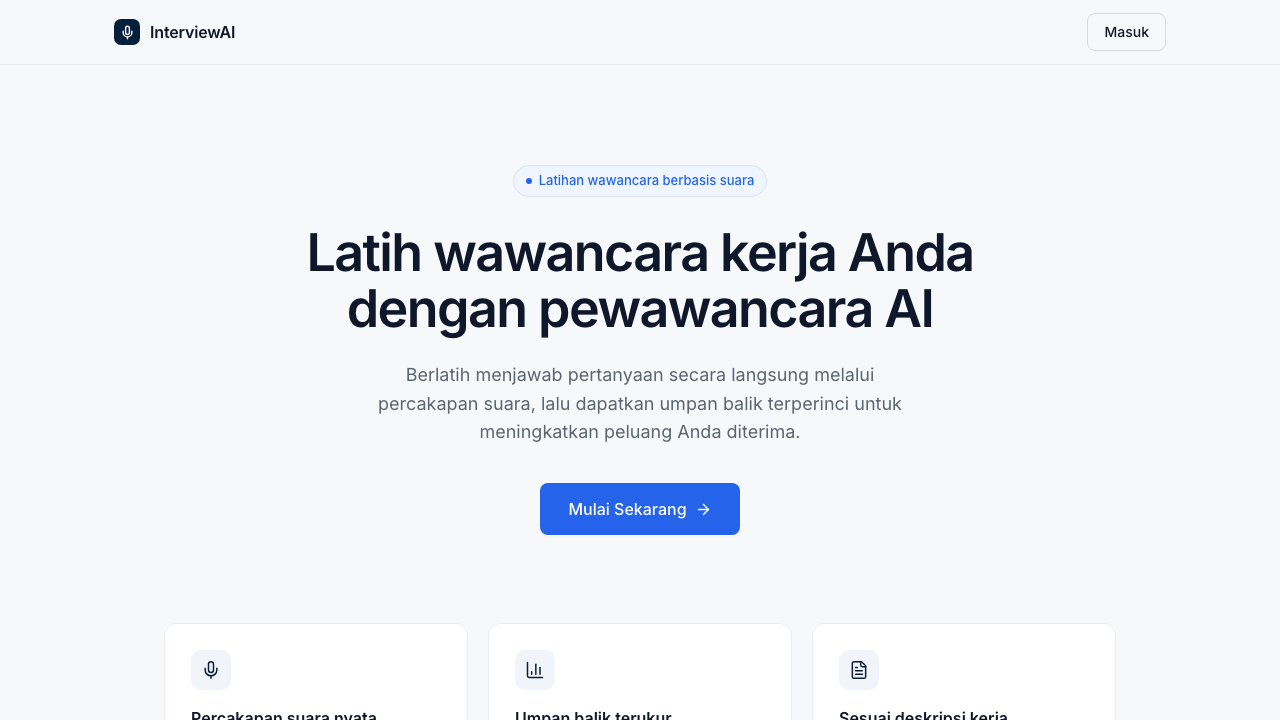
\includegraphics[width=\textwidth]{01-landing.png}
\caption{Halaman Landing}
\label{fig:landing}
\end{figure}

\begin{figure}[H]
\centering
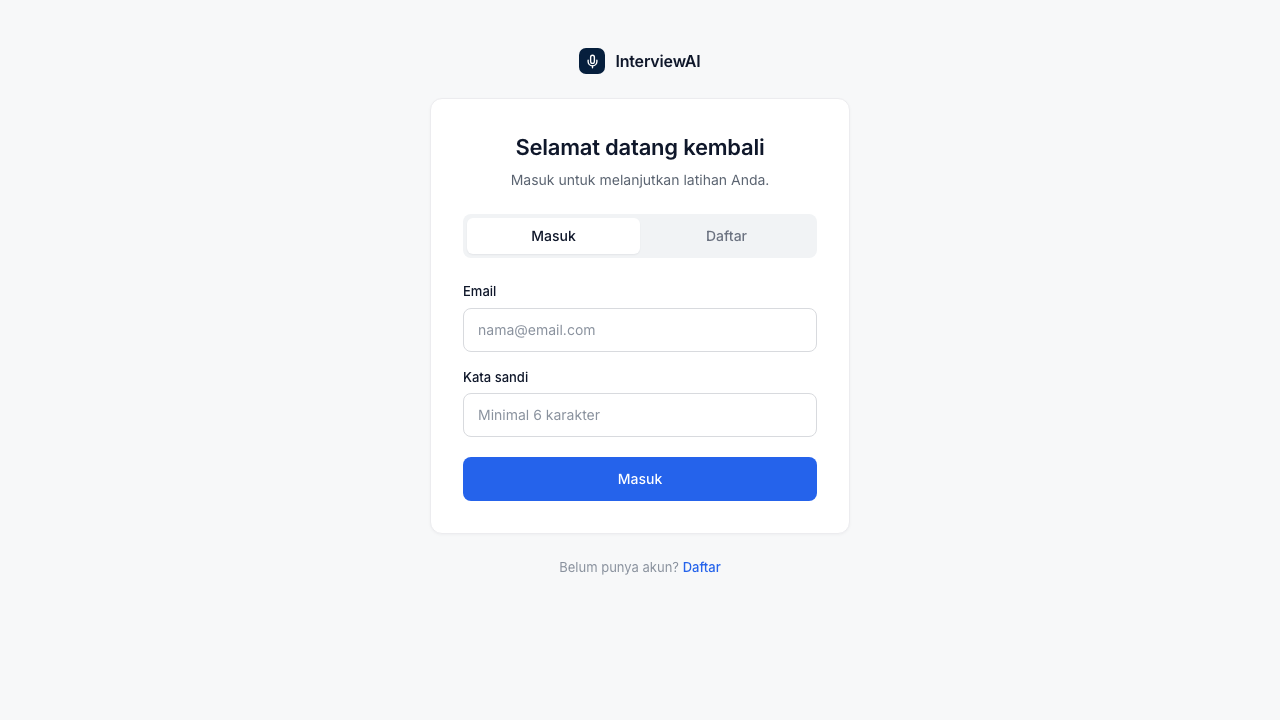
\includegraphics[width=0.8\textwidth]{02-login.png}
\caption{Halaman Login}
\label{fig:login}
\end{figure}

\begin{figure}[H]
\centering
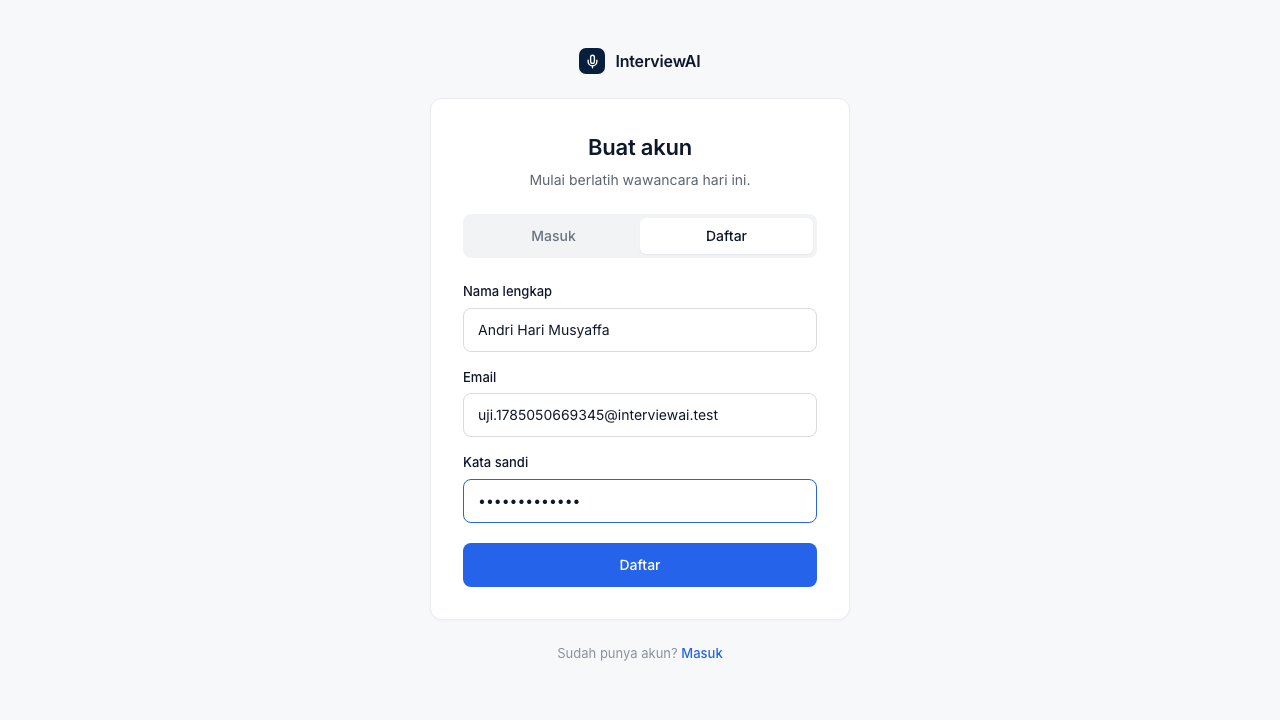
\includegraphics[width=0.8\textwidth]{03-register.png}
\caption{Halaman Register}
\label{fig:register}
\end{figure}

\begin{figure}[H]
\centering
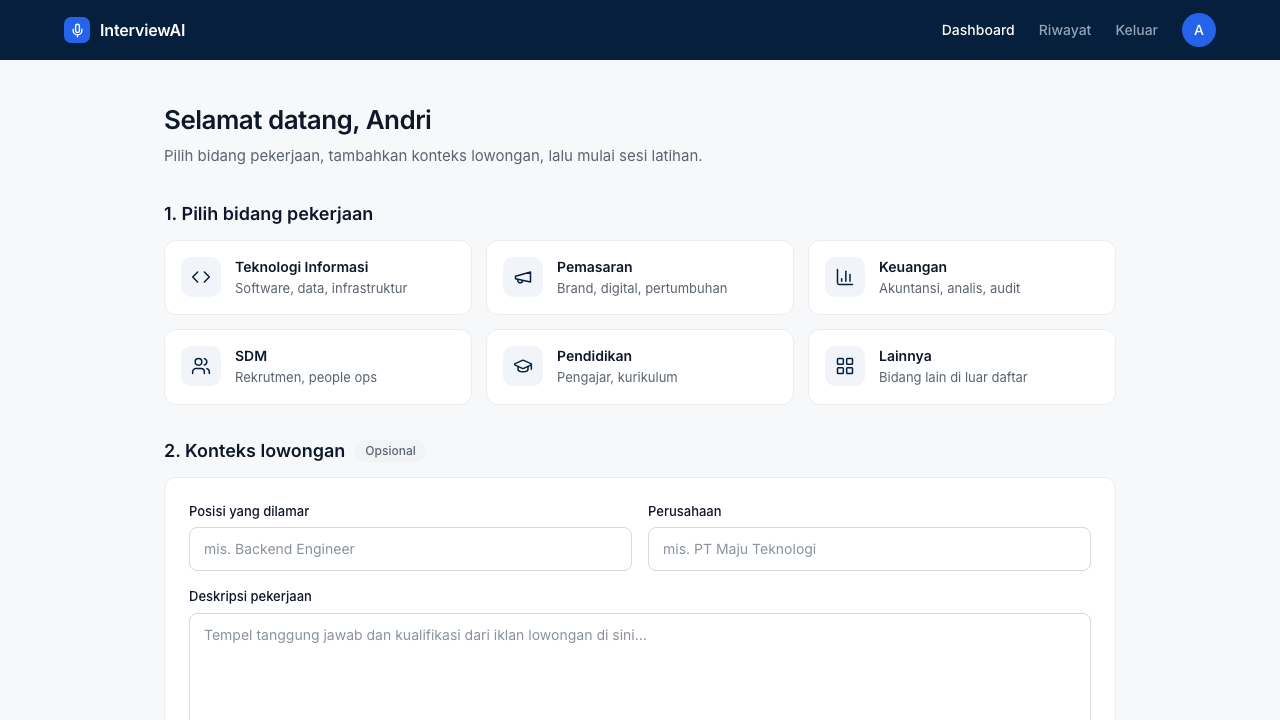
\includegraphics[width=\textwidth]{04-dashboard.png}
\caption{Halaman Dashboard --- Pemilihan Bidang Pekerjaan}
\label{fig:dashboard}
\end{figure}

\begin{figure}[H]
\centering
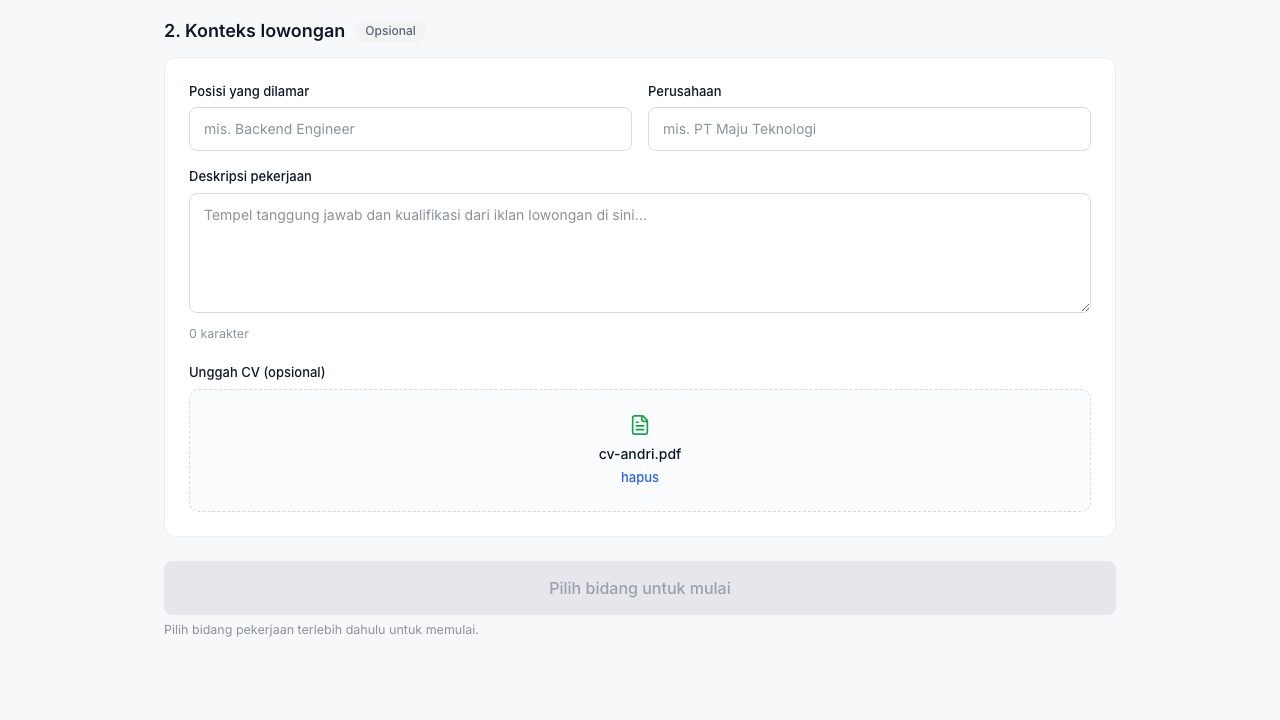
\includegraphics[width=\textwidth]{05-upload-cv.png}
\caption{Formulir Konteks Lowongan dan Unggah CV}
\label{fig:upload-cv}
\end{figure}

\begin{figure}[H]
\centering
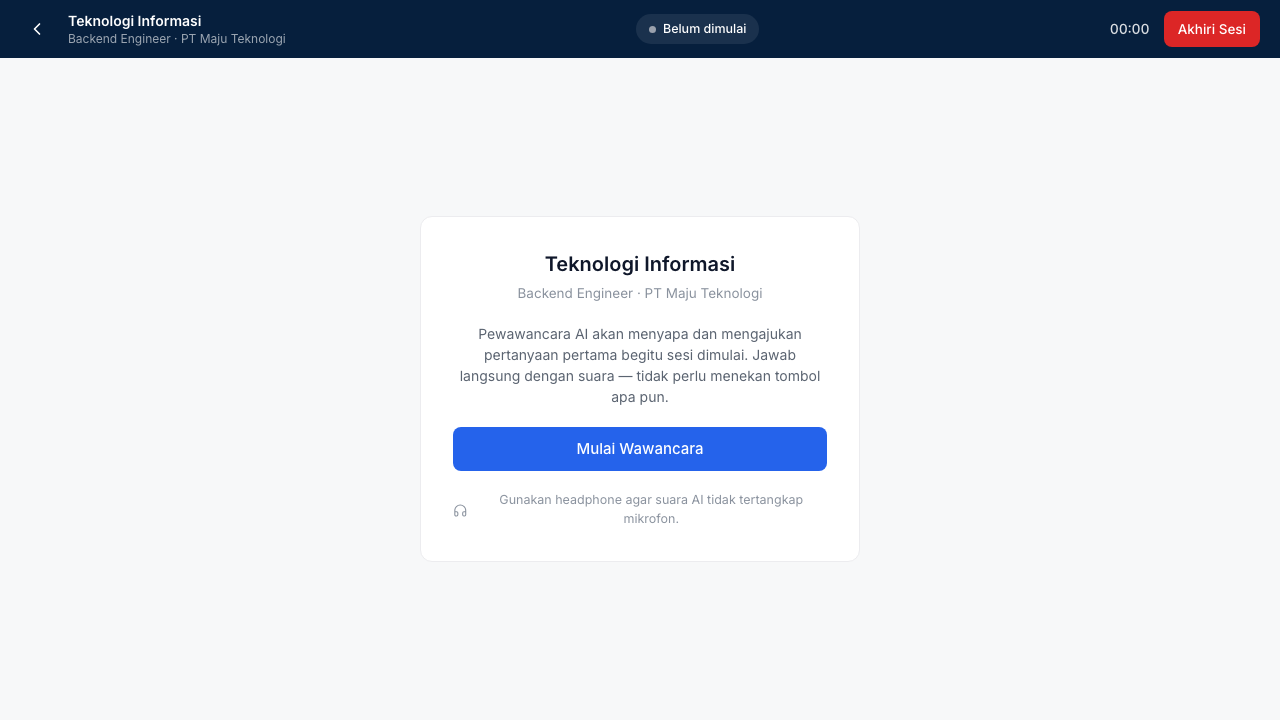
\includegraphics[width=\textwidth]{06-pre-session.png}
\caption{Halaman Persiapan Sesi Wawancara}
\label{fig:pre-session}
\end{figure}

\begin{figure}[H]
\centering
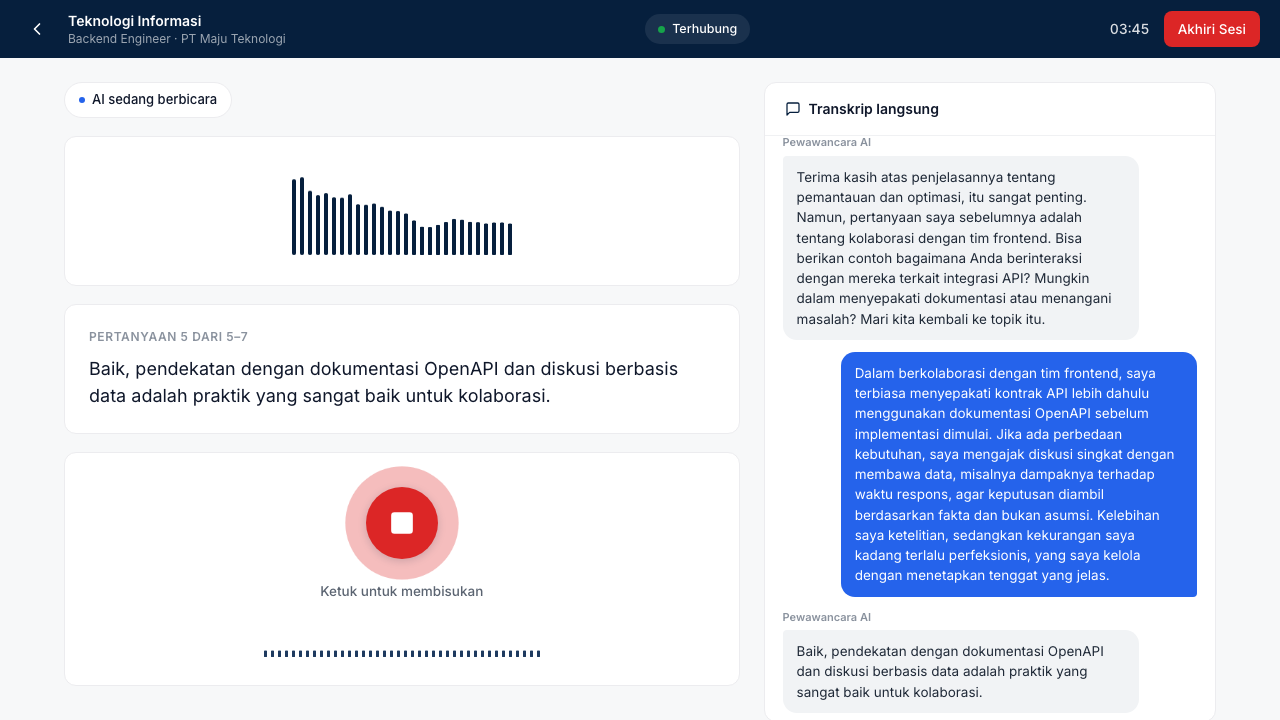
\includegraphics[width=\textwidth]{07-session-live.png}
\caption{Halaman Sesi Wawancara Berlangsung}
\label{fig:session-live}
\end{figure}

Gambar~\ref{fig:session-live} memperlihatkan sesi wawancara yang sedang
berjalan. Kolom kiri menampilkan indikator status pembicara, visualisasi
amplitudo audio, kartu pertanyaan terakhir, dan kendali mikrofon; sedangkan
kolom kanan menampilkan transkrip percakapan secara berurutan. Indikator
``Terhubung'' pada bilah atas menandakan koneksi \textit{WebSocket} ke Gemini
Live API dalam keadaan aktif, dan penghitung waktu menunjukkan durasi sesi
yang sedang berjalan.

\begin{figure}[H]
\centering
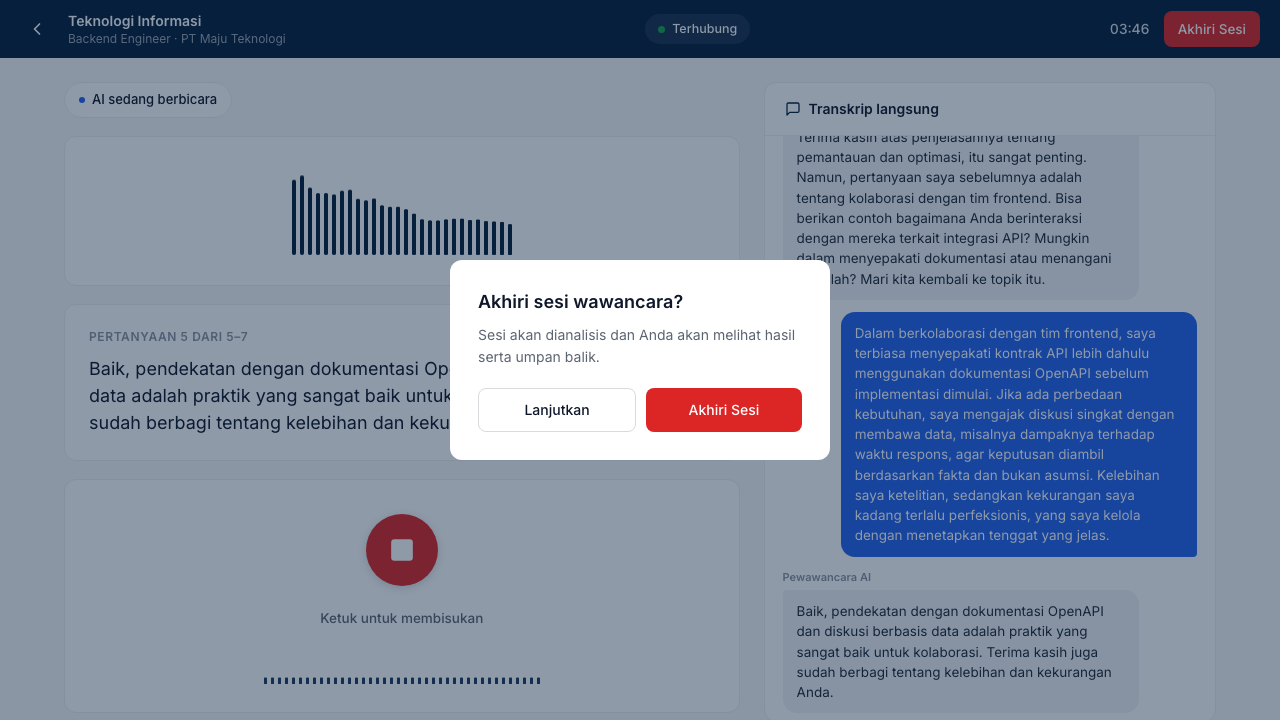
\includegraphics[width=\textwidth]{08-end-confirm.png}
\caption{Dialog Konfirmasi Pengakhiran Sesi}
\label{fig:end-confirm}
\end{figure}

\begin{figure}[H]
\centering
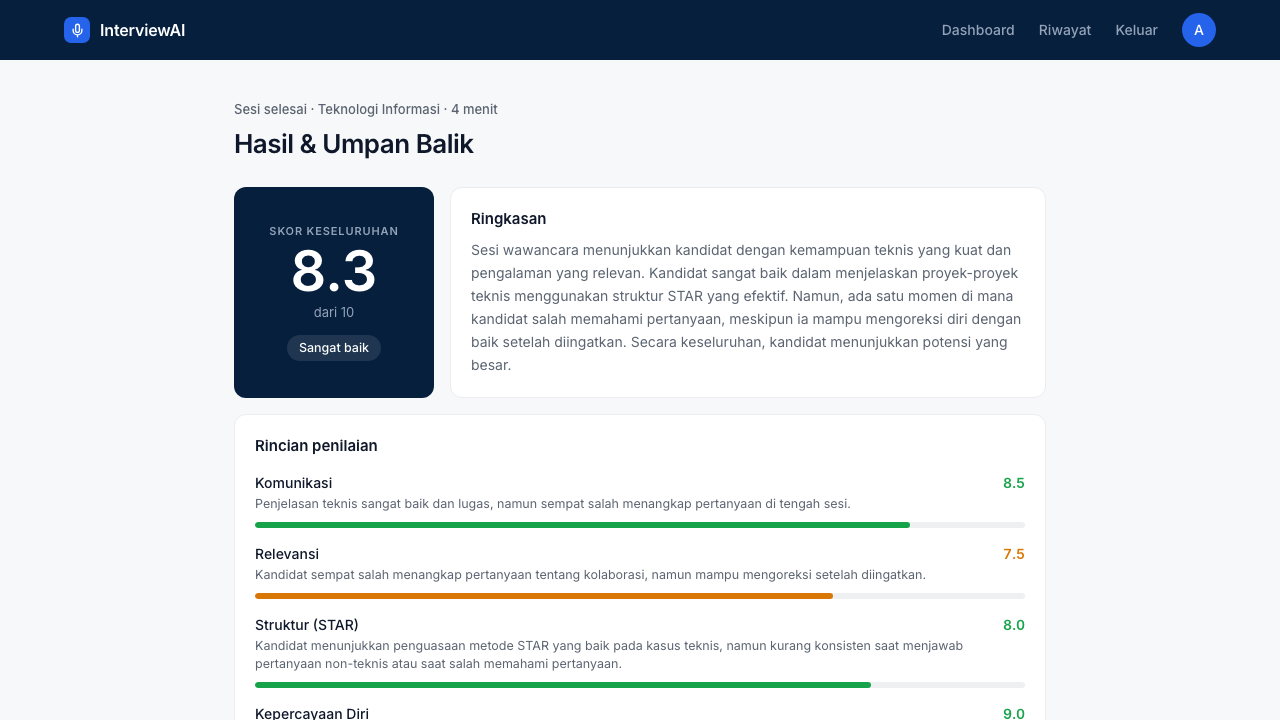
\includegraphics[width=\textwidth]{09-result.png}
\caption{Halaman Hasil dan Umpan Balik}
\label{fig:result}
\end{figure}

\begin{figure}[H]
\centering
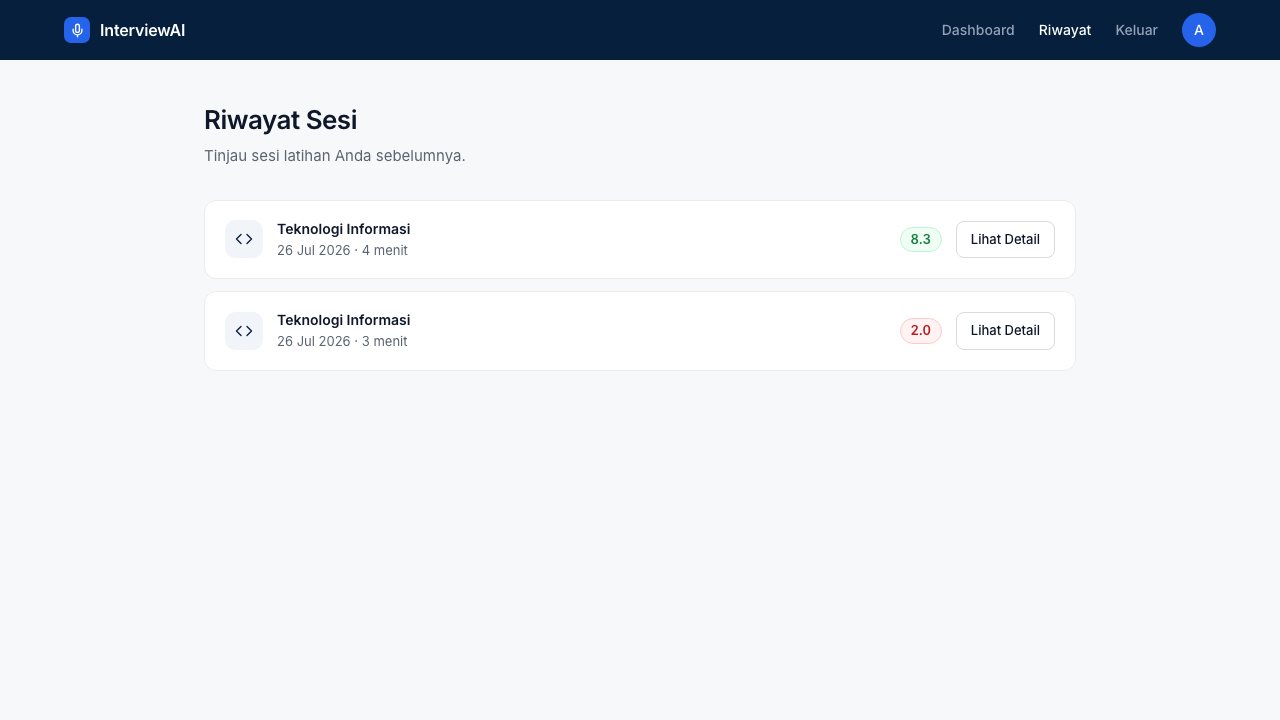
\includegraphics[width=\textwidth]{10-history.png}
\caption{Halaman Riwayat Sesi}
\label{fig:history}
\end{figure}

\begin{figure}[H]
\centering
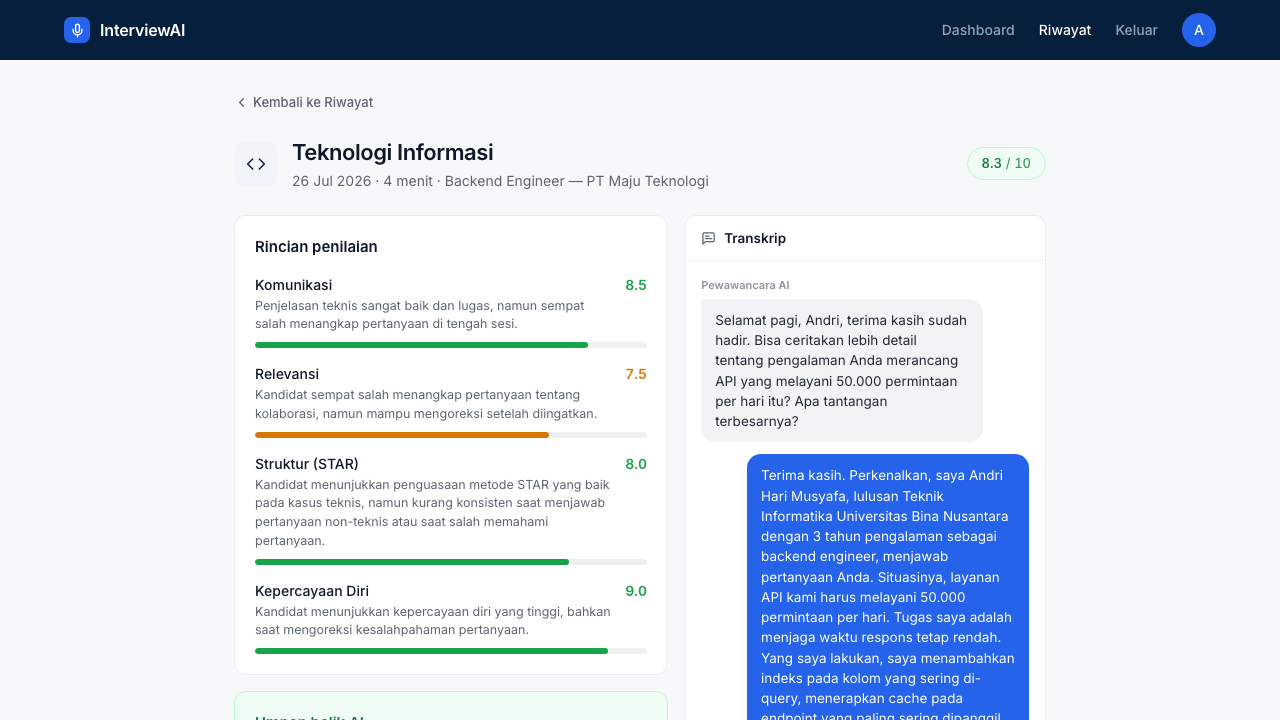
\includegraphics[width=\textwidth]{11-history-detail.png}
\caption{Halaman Detail Riwayat Sesi}
\label{fig:history-detail}
\end{figure}

\subsection{Implementasi Integrasi Gemini Live API}

Integrasi dengan Gemini Live API merupakan bagian paling kompleks dari sistem
ini karena melibatkan komunikasi audio dua arah secara \textit{real-time}.
Implementasinya menerapkan pola \textit{token broker}, yaitu \textit{backend}
tidak meneruskan aliran audio, melainkan hanya menerbitkan
\textit{ephemeral token} berumur pendek yang kemudian digunakan peramban untuk
membuka koneksi \textit{WebSocket Secure} langsung ke Gemini.

Alur satu sesi wawancara berjalan sebagai berikut:

\begin{enumerate}[leftmargin=*,itemsep=2pt]
  \item Pengguna memilih bidang pekerjaan, mengisi konteks lowongan, dan
        secara opsional mengunggah CV, lalu sistem membuat data sesi melalui
        \texttt{POST /api/sessions}.
  \item Peramban meminta \textit{ephemeral token} melalui
        \texttt{POST /api/sessions/:id/token}. Pada titik inilah
        \textit{backend} menyusun \textit{system instruction} yang berisi
        persona pewawancara beserta konteks sesi dan teks CV, lalu menguncinya
        di sisi server melalui \texttt{liveConnectConstraints}.
  \item Peramban membuka koneksi \textit{WebSocket} langsung ke Gemini
        menggunakan token tersebut, lalu mengirimkan perintah pembuka agar AI
        menyapa dan langsung mengajukan pertanyaan pertama.
  \item Audio mikrofon direkam pada 16 kHz, dikonversi menjadi PCM 16-bit di
        dalam \textit{AudioWorklet}, dan dikirimkan secara terus-menerus.
        Balasan audio Gemini pada 24 kHz diantrikan dan diputar kembali.
  \item Ketika pengguna mengakhiri sesi, transkrip dikirim ke
        \texttt{POST /api/sessions/}\linebreak[1]\texttt{:id/analyze} untuk dievaluasi, kemudian
        \texttt{POST /api/sessions/:id/end} menuliskan transkrip ke MongoDB
        lebih dahulu sebelum menandai sesi sebagai selesai di PostgreSQL.
\end{enumerate}

Parameter konfigurasi Gemini Live API hasil implementasi ditunjukkan pada
Tabel~\ref{tab:param-live}.

\begin{table}[H]
\caption{Parameter Konfigurasi Gemini Live API Hasil Implementasi}
\label{tab:param-live}
\centering
\begin{tabularx}{\textwidth}{|L{3.4cm}|L{4.2cm}|X|}
\hline
\textbf{Parameter} & \textbf{Nilai} & \textbf{Keterangan} \\
\hline
\textit{Model} & \texttt{gemini-3.1-flash-}\linebreak\texttt{live-preview} & Model \textit{native audio} dengan latensi terendah yang tersedia \\
\hline
Versi API & \texttt{v1alpha} & Versi yang menyediakan \textit{ephemeral token} \\
\hline
\textit{Response modalities} & \texttt{AUDIO} & Keluaran utama berupa audio \\
\hline
Transkripsi & \textit{input} dan \textit{output} diaktifkan & Menghasilkan transkrip dua arah untuk layar dan evaluasi \\
\hline
Format audio masuk & PCM 16-bit, 16 kHz, mono & Format yang diminta Gemini Live API \\
\hline
Format audio keluar & PCM 16-bit, 24 kHz, mono & Format balasan Gemini \\
\hline
\textit{Language code} & \texttt{id-ID} & Bahasa Indonesia \\
\hline
\textit{Voice} & \texttt{Kore} & Suara pewawancara AI \\
\hline
\textit{Temperature} & 0,7 & Keseimbangan variasi dan konsistensi respons \\
\hline
Masa berlaku token & 30 menit, sekali pakai & Membatasi dampak apabila token bocor \\
\hline
\end{tabularx}
\end{table}

\subsection{Implementasi Personalisasi Berbasis CV}

Berkas CV yang diunggah dalam format PDF maupun DOCX diekstraksi teksnya di
sisi \textit{backend}, lalu disisipkan ke dalam \textit{system instruction}
dengan batas maksimum 8.000 karakter. Pembatasan ini diperlukan karena
\textit{prompt} yang terlalu panjang meningkatkan biaya token sekaligus
latensi pada setiap sesi.

Efektivitas personalisasi ini terbukti pada saat pengujian. CV yang digunakan
memuat butir pengalaman berupa perancangan layanan API yang melayani 50.000
permintaan per hari. Pertanyaan pertama yang diajukan pewawancara AI adalah:

\begin{quote}
\textit{``Selamat pagi, Andri, terima kasih sudah hadir. Bisa ceritakan lebih
detail tentang pengalaman Anda merancang API yang melayani 50.000 permintaan
per hari itu? Apa tantangan terbesarnya?''}
\end{quote}

Pertanyaan tersebut menyebut angka yang hanya terdapat di dalam berkas CV,
sehingga membuktikan bahwa teks CV benar-benar terekstraksi, tersisipkan ke
dalam \textit{system instruction}, dan digunakan oleh model untuk menyusun
pertanyaan yang personal.

\subsection{Implementasi Evaluasi Terstruktur}

Evaluasi tidak dihasilkan oleh model percakapan, melainkan oleh model teks
terpisah (\texttt{gemini-2.5-flash}) yang menerima seluruh transkrip sesi.
Model diminta mengembalikan keluaran JSON terstruktur melalui mekanisme
\textit{response schema}, dengan empat metrik tetap yaitu Komunikasi,
Relevansi, Struktur (STAR), dan Kepercayaan Diri.

Karena keluaran model bahasa tetap berpotensi menyimpang dari skema yang
diminta, hasilnya melewati proses normalisasi sebelum disimpan. Proses ini
mencocokkan metrik berdasarkan \textit{key} maupun \textit{label},
membatasi setiap skor pada rentang 0--100, serta mengisi nilai cadangan
apabila ada bagian yang kosong. Dengan demikian bentuk data evaluasi yang
diterima antarmuka selalu konsisten, meskipun respons model bervariasi.

\subsection{Implementasi Keamanan}

Aspek keamanan yang berhasil diimplementasikan dirangkum pada
Tabel~\ref{tab:keamanan}.

\begin{table}[H]
\caption{Mekanisme Keamanan yang Diimplementasikan}
\label{tab:keamanan}
\centering
\begin{tabularx}{\textwidth}{|L{4.4cm}|X|}
\hline
\textbf{Aspek} & \textbf{Implementasi} \\
\hline
Kerahasiaan kunci API & Kunci API Gemini hanya berada di \textit{backend}; peramban hanya menerima \textit{ephemeral token} sekali pakai berumur 30 menit \\
\hline
Integritas persona AI & Model, \textit{system instruction}, suara, dan \textit{temperature} dikunci di sisi server; klien hanya boleh mengirim \textit{session resumption handle} \\
\hline
Autentikasi & JWT \textit{access token} berumur 15 menit dan \textit{refresh token} 7 hari pada \textit{cookie} \texttt{httpOnly} \\
\hline
Penyimpanan kata sandi & \textit{Hashing} menggunakan algoritma Argon2 \\
\hline
Pembatasan laju & 20 permintaan per IP tiap 15 menit pada \textit{endpoint} autentikasi, dan 40 permintaan per pengguna tiap 15 menit pada \textit{endpoint} yang memanggil Gemini \\
\hline
Otorisasi data & Setiap akses sesi maupun CV memverifikasi kepemilikan \texttt{user\_id}, dan parameter UUID divalidasi sebelum menyentuh basis data \\
\hline
Pengerasan HTTP & \textit{Helmet}, CORS dengan satu \textit{origin} dari variabel lingkungan, serta validasi variabel lingkungan saat proses \textit{boot} \\
\hline
\end{tabularx}
\end{table}

Pembatasan peran juga diterapkan pada tingkat \textit{prompt}. \textit{System
instruction} secara eksplisit melarang AI menjawab pertanyaan di luar konteks
wawancara serta mengabaikan permintaan untuk berganti peran atau membocorkan
isi instruksi, sebagai mitigasi terhadap upaya \textit{prompt injection}.

% =====================================================================
\section{Penyesuaian terhadap Rancangan BAB III}
% =====================================================================

Selama tahap implementasi ditemukan sejumlah kendala teknis yang menyebabkan
beberapa keputusan rancangan pada BAB III perlu disesuaikan. Ringkasan
penyesuaian tersebut ditunjukkan pada Tabel~\ref{tab:deviasi}, sedangkan
penyesuaian yang paling berdampak diuraikan pada sub-bab berikutnya.

\begin{table}[H]
\caption{Ringkasan Penyesuaian Rancangan terhadap Implementasi}
\label{tab:deviasi}
\centering
\begin{tabularx}{\textwidth}{|L{3.5cm}|L{3.4cm}|X|}
\hline
\textbf{Rancangan (BAB III)} & \textbf{Implementasi} & \textbf{Alasan Penyesuaian} \\
\hline
Supabase sebagai penyedia PostgreSQL, Auth, dan Storage & PostgreSQL mandiri, autentikasi JWT + Argon2 sendiri, CV disimpan pada \textit{filesystem} server & Menghilangkan ketergantungan pada layanan pihak ketiga dan biaya berlangganan, sekaligus memberi kendali penuh atas skema basis data dan masa berlaku token \\
\hline
\textit{Backend} berperan sebagai \textit{WebSocket proxy} & Pola \textit{token broker}; audio mengalir langsung dari peramban ke Gemini & \textit{Proxy} menambah satu lompatan jaringan pada jalur yang paling sensitif terhadap latensi dan membebani server dengan seluruh aliran audio. Pola \textit{token broker} tetap menjaga kerahasiaan kunci API tanpa biaya latensi tersebut \\
\hline
Model \texttt{gemini-live-}\linebreak\texttt{3-flash}, suara bawaan & \texttt{gemini-3.1-}\linebreak\texttt{flash-live-}\linebreak\texttt{preview}, suara \texttt{Kore}, \texttt{id-ID} & Nama model pada rancangan tidak tersedia. Model yang dipilih memberi waktu respons sekitar 1,5 detik dibanding sekitar 5,0 detik pada alternatifnya \\
\hline
Evaluasi berupa \texttt{overall\_score} dan \texttt{feedback\_text} & Ditambah empat metrik terstruktur, \texttt{strengths}, \texttt{improvements}, dan \texttt{summary} & Skor tunggal tidak cukup informatif sebagai bahan perbaikan. Penilaian per aspek menjawab kebutuhan umpan balik yang dapat ditindaklanjuti \\
\hline
Tipe kunci utama pada \texttt{job\_fields} adalah SERIAL & Bertipe UUID & Menyeragamkan tipe kunci seluruh tabel sehingga tidak ada identitas yang mudah ditebak berurutan \\
\hline
\textit{Deployment} pada Vercel dan Cloud Run & Direncanakan pada VPS di belakang \textit{nginx} & Menyederhanakan operasional menjadi satu lingkungan dan menekan biaya. Tahap ini belum dilaksanakan pada penelitian ini \\
\hline
\end{tabularx}
\end{table}

\subsection{Penggantian Supabase dengan Layanan Mandiri}

Rancangan awal menempatkan Supabase sebagai penyedia PostgreSQL, autentikasi,
dan penyimpanan berkas sekaligus. Pada implementasi, ketiga peran tersebut
dipisahkan dan dikelola sendiri. PostgreSQL dijalankan secara mandiri dengan
skema yang dikelola melalui berkas migrasi SQL berurutan, autentikasi
diimplementasikan menggunakan JWT dengan \textit{hashing} Argon2, dan berkas
CV disimpan pada \textit{filesystem} server dengan nama berkas yang diacak.

Konsekuensinya, pengelolaan keamanan autentikasi menjadi tanggung jawab
sistem ini sendiri. Hal tersebut dikompensasi dengan penerapan \textit{refresh
token} pada \textit{cookie} \texttt{httpOnly}, masa berlaku \textit{access
token} yang pendek, serta pembatasan laju pada \textit{endpoint}
autentikasi.

\subsection{Perubahan Pola Integrasi menjadi \textit{Token Broker}}

Perubahan paling mendasar terjadi pada pola integrasi dengan Gemini Live API.
Rancangan BAB III menempatkan \textit{backend} sebagai \textit{WebSocket
proxy} yang meneruskan audio dari klien ke Gemini. Pendekatan tersebut
memiliki dua kelemahan: seluruh aliran audio dua arah harus melewati server
sehingga menambah beban dan biaya bandwidth, dan setiap lompatan tambahan
menambah latensi pada jalur yang justru paling menentukan kealamian
percakapan.

Pada implementasi, \textit{backend} hanya berperan menerbitkan
\textit{ephemeral token}, sedangkan koneksi \textit{WebSocket} dibuka langsung
dari peramban ke Gemini. Kerahasiaan kunci API tetap terjaga karena kunci
tersebut tidak pernah meninggalkan server, dan konfigurasi sesi dikunci pada
saat token diterbitkan sehingga klien tidak dapat mengubah persona
pewawancara, model, maupun suara yang digunakan.

\subsection{Perluasan Skema Evaluasi}

Rancangan awal hanya menyimpan skor keseluruhan dan umpan balik naratif.
Skema tersebut diperluas menjadi empat metrik penilaian beserta catatannya,
ditambah daftar kelebihan, daftar hal yang perlu ditingkatkan, dan ringkasan
sesi. Perluasan ini menjawab tujuan penelitian mengenai umpan balik yang
bersifat personal, karena pengguna dapat mengetahui aspek mana yang lemah dan
bukan sekadar menerima satu angka.

% =====================================================================
\section{Pengujian Sistem}
% =====================================================================

\subsection{Metode dan Lingkungan Pengujian}

Pengujian dilakukan menggunakan metode \textit{Black Box Testing} sesuai
rencana pada BAB III, yaitu memvalidasi fungsionalitas berdasarkan masukan dan
keluaran yang diharapkan tanpa memeriksa struktur internal kode program.
Seluruh skenario diotomasi menggunakan Playwright dan dijalankan pada peramban
Chromium, sehingga pengujian dapat diulang dan hasilnya dapat diverifikasi
kembali.

Skenario dijalankan secara berurutan dalam satu \textit{worker} karena antar
skenario terdapat ketergantungan data: sesi wawancara yang diselesaikan pada
berkas skenario ketiga merupakan data yang diperiksa oleh skenario pengujian
riwayat. Dengan demikian alur simpan dan baca lintas kedua basis data ikut
terverifikasi.

Pengujian sesi wawancara suara memerlukan sumber suara kandidat. Suara
tersebut disintesis menggunakan \textit{text-to-speech} berbahasa Indonesia
berisi lima jawaban yang disusun mengikuti kerangka STAR, dengan jeda hening
di antara jawaban agar giliran bicara tidak bertabrakan dengan suara
pewawancara AI.

Pada tahap penyiapan ditemukan bahwa opsi Chromium
\texttt{-{}-use-file-for-}\allowbreak\texttt{fake-audio-capture} tidak berpengaruh pada
lingkungan pengujian yang digunakan. Hal ini diverifikasi menggunakan berkas
uji berpola nada keras dan hening bergantian setiap satu detik: pola tersebut
sama sekali tidak muncul pada data PCM yang benar-benar dikirimkan aplikasi ke
Gemini. Oleh karena itu mikrofon disimulasikan satu lapis lebih tinggi, yaitu
dengan mengembalikan \textit{MediaStream} yang dibangkitkan Web Audio API dari
berkas suara yang sama. Yang disimulasikan hanya perangkat keras mikrofonnya,
sedangkan seluruh jalur kode aplikasi --- \textit{AudioWorklet}, konversi PCM
16 kHz, hingga pengiriman ke Gemini --- tetap berjalan apa adanya, sehingga
pengujian tetap sah sebagai pengujian \textit{Black Box} terhadap sistem.

\subsection{Skenario dan Hasil Pengujian}

Sebanyak 26 skenario pengujian disusun untuk mencakup kesebelas
\textit{use case} yang dirancang pada BAB III, mencakup kasus normal maupun
kasus negatif. Hasil pengujian selengkapnya ditunjukkan pada
Tabel~\ref{tab:hasil-uji}.

\begin{longtable}{|C{1.1cm}|C{1.1cm}|L{4.5cm}|L{3.1cm}|C{1.3cm}|}
\caption{Hasil Pengujian \textit{Black Box}}
\label{tab:hasil-uji} \\
\hline
\textbf{Kode} & \textbf{UC} & \textbf{Skenario Pengujian} & \textbf{Hasil yang Diharapkan} & \textbf{Hasil} \\
\hline
\endfirsthead
\multicolumn{5}{l}{\small\textit{Lanjutan Tabel \ref{tab:hasil-uji}}} \\
\hline
\textbf{Kode} & \textbf{UC} & \textbf{Skenario Pengujian} & \textbf{Hasil yang Diharapkan} & \textbf{Hasil} \\
\hline
\endhead
\hline
\endfoot
\hline
\endlastfoot

TC-00 & -- & Membuka halaman Landing & Judul dan tombol ``Mulai Sekarang'' tampil & Valid \\
\hline
TC-01 & UC-02 & Membuka Dashboard tanpa autentikasi & Dialihkan ke halaman Login & Valid \\
\hline
TC-02 & UC-01 & Register dengan format email tidak valid & Pesan ``Masukkan email yang valid'' tampil & Valid \\
\hline
TC-03 & UC-01 & Register dengan kata sandi kurang dari 6 karakter & Pesan ``Kata sandi minimal 6 karakter'' tampil & Valid \\
\hline
TC-04 & UC-01 & Register dengan data lengkap dan valid & Akun terbentuk dan masuk ke Dashboard & Valid \\
\hline
TC-05 & UC-01 & Register dengan email yang sudah terdaftar & Ditolak server dengan pesan galat & Valid \\
\hline
TC-06 & UC-02 & Login dengan kata sandi salah & Ditolak dan tetap di halaman Login & Valid \\
\hline
TC-07 & UC-02 & Login dengan kredensial benar & Masuk ke Dashboard & Valid \\
\hline
TC-08 & UC-10 & Menekan tombol Keluar & Sesi berakhir dan halaman terproteksi diblokir & Valid \\
\hline
TC-09 & UC-03 & Memuat daftar bidang pekerjaan & Enam bidang pekerjaan tampil dari server & Valid \\
\hline
TC-10 & UC-03 & Belum memilih bidang pekerjaan & Tombol mulai sesi dalam keadaan nonaktif & Valid \\
\hline
TC-11 & UC-03 & Memilih salah satu bidang pekerjaan & Tombol mulai sesi menjadi aktif & Valid \\
\hline
TC-12 & UC-03 & Mengisi deskripsi lowongan lebih dari 40 karakter & Konfirmasi ``Konteks akan dipakai AI'' tampil & Valid \\
\hline
TC-13 & UC-11 & Mengunggah CV berformat PDF & Berkas terunggah dan teksnya terekstraksi & Valid \\
\hline
TC-14 & UC-11 & Mengunggah CV berformat DOCX & Berkas terunggah dan teksnya terekstraksi & Valid \\
\hline
TC-15 & UC-11 & Mengunggah berkas berformat selain PDF/DOCX & Ditolak dengan pesan format tidak sesuai & Valid \\
\hline
TC-16 & UC-11 & Menghapus CV yang telah diunggah & Formulir kembali ke keadaan semula & Valid \\
\hline
TC-17 & UC-04 & Menekan tombol Mulai Sesi Wawancara & Sesi terbentuk dan halaman wawancara terbuka & Valid \\
\hline
TC-18 & UC-04 & Memulai wawancara & Koneksi terbuka dan AI menyapa serta bertanya & Valid \\
\hline
TC-19 & UC-05 & Kandidat menjawab dengan suara & Jawaban tertranskripsi pada panel transkrip & Valid \\
\hline
TC-20 & UC-06 & Melanjutkan percakapan beberapa giliran & AI menanggapi jawaban dan mengajukan pertanyaan lanjutan & Valid \\
\hline
TC-21 & UC-07 & Mengakhiri sesi wawancara & Evaluasi dihasilkan dan halaman Hasil tampil lengkap & Valid \\
\hline
TC-22 & UC-08 & Membuka halaman Riwayat & Sesi yang telah selesai tampil beserta skornya & Valid \\
\hline
TC-23 & UC-09 & Membuka detail salah satu sesi & Rincian penilaian dan transkrip tampil & Valid \\
\hline
TC-24 & UC-09 & Membuka detail sesi milik pengguna lain & Akses ditolak dan pesan galat tampil & Valid \\
\hline
TC-25 & UC-09 & Kembali dari detail ke daftar riwayat & Kembali ke halaman Riwayat & Valid \\
\hline
\end{longtable}

\subsection{Analisis Persentase Keberhasilan}

Persentase keberhasilan dihitung menggunakan rumus yang telah ditetapkan pada
BAB III, yaitu:

\begin{center}
\textit{Success Rate} $=\dfrac{\text{Jumlah \textit{test case} valid}}{\text{Total \textit{test case}}}\times 100\%$
\end{center}

Rekapitulasi hasil pengujian per \textit{use case} ditunjukkan pada
Tabel~\ref{tab:success-rate}.

\begin{table}[H]
\caption{Rekapitulasi Persentase Keberhasilan per \textit{Use Case}}
\label{tab:success-rate}
\centering
\begin{tabularx}{\textwidth}{|C{1.6cm}|X|C{1.9cm}|C{1.6cm}|C{2.1cm}|}
\hline
\textbf{Kode UC} & \textbf{Nama \textit{Use Case}} & \textbf{Jumlah \textit{Test Case}} & \textbf{Valid} & \textbf{Persentase} \\
\hline
UC-01 & Register & 4 & 4 & 100\% \\
\hline
UC-02 & Login & 3 & 3 & 100\% \\
\hline
UC-03 & Memilih Bidang Pekerjaan & 4 & 4 & 100\% \\
\hline
UC-04 & Memulai Sesi Wawancara & 2 & 2 & 100\% \\
\hline
UC-05 & Menjawab Pertanyaan & 1 & 1 & 100\% \\
\hline
UC-06 & Menerima Umpan Balik & 1 & 1 & 100\% \\
\hline
UC-07 & Mengakhiri Sesi & 1 & 1 & 100\% \\
\hline
UC-08 & Melihat Riwayat Sesi & 1 & 1 & 100\% \\
\hline
UC-09 & Melihat Detail Riwayat & 3 & 3 & 100\% \\
\hline
UC-10 & Logout & 1 & 1 & 100\% \\
\hline
UC-11 & Mengunggah CV & 4 & 4 & 100\% \\
\hline
-- & Umum (halaman Landing) & 1 & 1 & 100\% \\
\hline
\multicolumn{2}{|c|}{\textbf{Total}} & \textbf{26} & \textbf{26} & \textbf{100\%} \\
\hline
\end{tabularx}
\end{table}

Berdasarkan rekapitulasi tersebut, seluruh 26 \textit{test case} dinyatakan
valid sehingga persentase keberhasilan mencapai 100\%. Nilai ini melampaui
ambang minimal 90\% untuk setiap kategori fitur yang ditetapkan pada BAB III,
sehingga hipotesis penelitian mengenai keberhasilan fungsional sistem
dinyatakan terpenuhi.

% =====================================================================
\section{Pembahasan}
% =====================================================================

\subsection{Ketercapaian Tujuan Penelitian}

Rumusan masalah pertama mempertanyakan bagaimana merancang dan membangun
\textit{website} simulasi wawancara kerja berbasis \textit{Large Language
Model} dengan memanfaatkan Gemini Live API. Hasil implementasi menunjukkan
bahwa sistem tersebut berhasil dibangun secara utuh, mulai dari autentikasi,
konfigurasi sesi, wawancara suara \textit{real-time}, evaluasi otomatis,
hingga riwayat sesi. Sistem berjalan sepenuhnya di dalam peramban tanpa
memerlukan pemasangan perangkat lunak tambahan, dan seluruh antarmukanya
menggunakan Bahasa Indonesia sehingga dapat diakses oleh pencari kerja di
Indonesia tanpa hambatan bahasa maupun biaya sesi.

Rumusan masalah kedua mempertanyakan bagaimana mengintegrasikan fitur
pertanyaan otomatis, penilaian jawaban, umpan balik personal, dan komunikasi
suara \textit{real-time} ke dalam satu \textit{platform} berbasis web.
Keempat fitur tersebut terbukti berjalan dalam satu alur yang berkesinambungan
sebagaimana ditunjukkan pada pengujian TC-17 sampai TC-21. Pertanyaan
dihasilkan secara otomatis dan dipersonalisasi berdasarkan CV, jawaban
disampaikan melalui suara dan tertranskripsi, umpan balik lisan diberikan di
sela percakapan, serta penilaian tertulis per aspek disajikan setelah sesi
berakhir.

\subsection{Analisis Kinerja Percakapan \textit{Real-time}}

Pengukuran kinerja diambil langsung pada saat pengujian sesi wawancara
berlangsung dan dirangkum pada Tabel~\ref{tab:kinerja}.

\begin{table}[H]
\caption{Hasil Pengukuran Kinerja Sesi Wawancara}
\label{tab:kinerja}
\centering
\begin{tabularx}{\textwidth}{|X|C{3cm}|}
\hline
\textbf{Aspek yang Diukur} & \textbf{Hasil} \\
\hline
Waktu dari penekanan tombol mulai hingga AI mengucapkan sapaan pertama & 2,2 detik \\
\hline
Waktu dari mulai berbicara hingga jawaban muncul pada panel transkrip & 58,1 detik\footnotemark \\
\hline
Jumlah giliran bicara pewawancara AI dalam satu sesi & 5 giliran \\
\hline
Jumlah giliran bicara kandidat dalam satu sesi & 4 giliran \\
\hline
Total panjang transkrip jawaban kandidat & 1.856 karakter \\
\hline
Waktu pembuatan evaluasi setelah sesi diakhiri & 11,9 detik \\
\hline
\end{tabularx}
\end{table}
\footnotetext{Angka ini mencakup jeda hening 17 detik pada awal berkas suara
uji dan durasi pengucapan jawaban itu sendiri, sehingga bukan merupakan
latensi transkripsi murni. Latensi transkripsi terukur berada pada kisaran 3
detik di belakang penutur.}

Waktu tanggap awal sebesar 2,2 detik menunjukkan bahwa pola \textit{token
broker} tidak menimbulkan penundaan yang terasa, meskipun peramban harus
meminta token ke \textit{backend} terlebih dahulu sebelum membuka koneksi ke
Gemini. Adapun waktu pembuatan evaluasi sebesar 11,9 detik masih dapat
diterima karena berlangsung sekali di akhir sesi dan disertai indikator
pemuatan pada antarmuka.

Karakteristik penting yang ditemukan pada tahap implementasi adalah bahwa
transkripsi masukan dari Gemini berjalan sekitar tiga detik di belakang
penutur. Akibatnya, indikator ``sedang berbicara'' pada antarmuka tidak dapat
mengandalkan transkrip tersebut. Sistem mengatasinya dengan mendeteksi
amplitudo suara secara lokal di peramban, dan sinyal tersebut digunakan
semata-mata untuk keperluan tampilan, tidak pernah untuk menggerbang
pengiriman audio ke Gemini.

\subsection{Analisis Kualitas Evaluasi}

Selama tahap pengujian dilakukan dua kali sesi wawancara dengan naskah jawaban
yang berbeda, dan perbandingan hasilnya ditunjukkan pada
Tabel~\ref{tab:banding-evaluasi}.

\begin{table}[H]
\caption{Perbandingan Hasil Evaluasi terhadap Dua Naskah Jawaban}
\label{tab:banding-evaluasi}
\centering
\begin{tabularx}{\textwidth}{|X|C{2.4cm}|C{2.4cm}|}
\hline
\textbf{Karakteristik Naskah Jawaban} & \textbf{Skor Keseluruhan} & \textbf{Skor Relevansi} \\
\hline
Jawaban umum yang tidak menanggapi pertanyaan spesifik pewawancara & 2,0 & 1,5 \\
\hline
Jawaban terstruktur STAR yang menanggapi pokok pertanyaan & 8,3 & tinggi \\
\hline
\end{tabularx}
\end{table}

Perbedaan skor yang lebar antara kedua naskah menunjukkan bahwa mekanisme
evaluasi bersifat diskriminatif, yaitu benar-benar menilai isi dan relevansi
jawaban dan bukan sekadar memberikan skor tinggi secara seragam. Pada naskah
pertama, sistem secara tepat mengidentifikasi bahwa kandidat berulang kali
tidak menjawab pertanyaan yang diajukan, dan hal tersebut tercermin pada skor
Relevansi yang rendah. Temuan ini memperkuat keyakinan bahwa umpan balik yang
dihasilkan sistem memiliki nilai diagnostik bagi pengguna.

\subsection{Keterbatasan Sistem}

Berdasarkan hasil implementasi dan pengujian, terdapat sejumlah keterbatasan
yang perlu dicatat:

\begin{enumerate}[leftmargin=*,itemsep=3pt]
  \item \textbf{Ketergantungan pada model \textit{preview}.} Model
        \texttt{gemini-3.1-flash-}\allowbreak\texttt{live-preview} berstatus
        \textit{preview}
        sehingga berpotensi berubah atau dihentikan sewaktu-waktu. Sistem
        belum memiliki mekanisme peralihan otomatis ke model cadangan.
  \item \textbf{Penentuan batas giliran bicara bersifat heuristik.} Karena
        Gemini tidak menyertakan penanda waktu pengucapan pada setiap potongan
        transkrip, sistem menentukan giliran berdasarkan waktu kedatangan
        data. Pada kondisi tertentu, beberapa kata terakhir sebuah jawaban
        dapat tergeser ke giliran berikutnya, meskipun isi dan urutan
        percakapan secara keseluruhan tetap terjaga.
  \item \textbf{Penilaian terbatas pada aspek verbal.} Sesuai ruang lingkup
        pada BAB III, sistem tidak menilai aspek psikologis maupun bahasa
        tubuh, karena masukannya hanya berupa suara.
  \item \textbf{Pengujian belum mencakup keberagaman pengguna nyata.}
        Pengujian dilakukan menggunakan suara sintetis pada satu lingkungan
        peramban. Variasi aksen, kecepatan bicara, kualitas mikrofon, dan
        kondisi kebisingan pengguna nyata belum terwakili.
  \item \textbf{Tahap \textit{deployment} belum dilaksanakan.} Sistem baru
        berjalan pada lingkungan pengembangan lokal, sehingga pengujian
        performa pada kondisi produksi belum dapat dilakukan.
\end{enumerate}

\end{document}
